\documentclass[oneside]{utmthesis}
% Options
% Size [a4draft, b5final]
% Language [english, malay]
% Printing [twoside, oneside]
% Default option [a4draft, english, twoside]

\usepackage{graphicx}
\usepackage{url} 
\usepackage{pdflscape}
\usepackage{longtable}
\usepackage{notoccite}
\usepackage[numbers]{natbib}
\usepackage{multirow}%
\usepackage{algorithm}
\usepackage{algpseudocode}
\usepackage{array}%
\usepackage{color,soul}%
 \usepackage[table,xcdraw]{xcolor}


\usepackage{booktabs}
\usepackage[caption=false]{subfig}
\newcolumntype{P}[1]{>{\centering\arraybackslash}m{#1}}%

%This is to make sure vertical spacing non-stretchable
\raggedbottom


% Required information
\title{LexiFlow: A Web Platform for Translating and Transcribing Native Mandarin Content}

\author{Adam Ismail Hassan Amer Abouraya}
% \metricno{A22EC0002}
% \dob{26 July 2025}
\degree{Bachelor of Computer Science}
\specialization{Software Engineering}
\intakeyear{2022}
\faculty{Faculty of Computing}
\titledate{July 2025}
% \titleyear{2025}
% \semester{2024/2025-2}
% \signingdate{25 June 2025}

\award{1}

\superone{Dr.~Shahliza Binti Abd Halim}




\begin{document}


% ----------------------------------------------------------------
\coverpage
\superpage
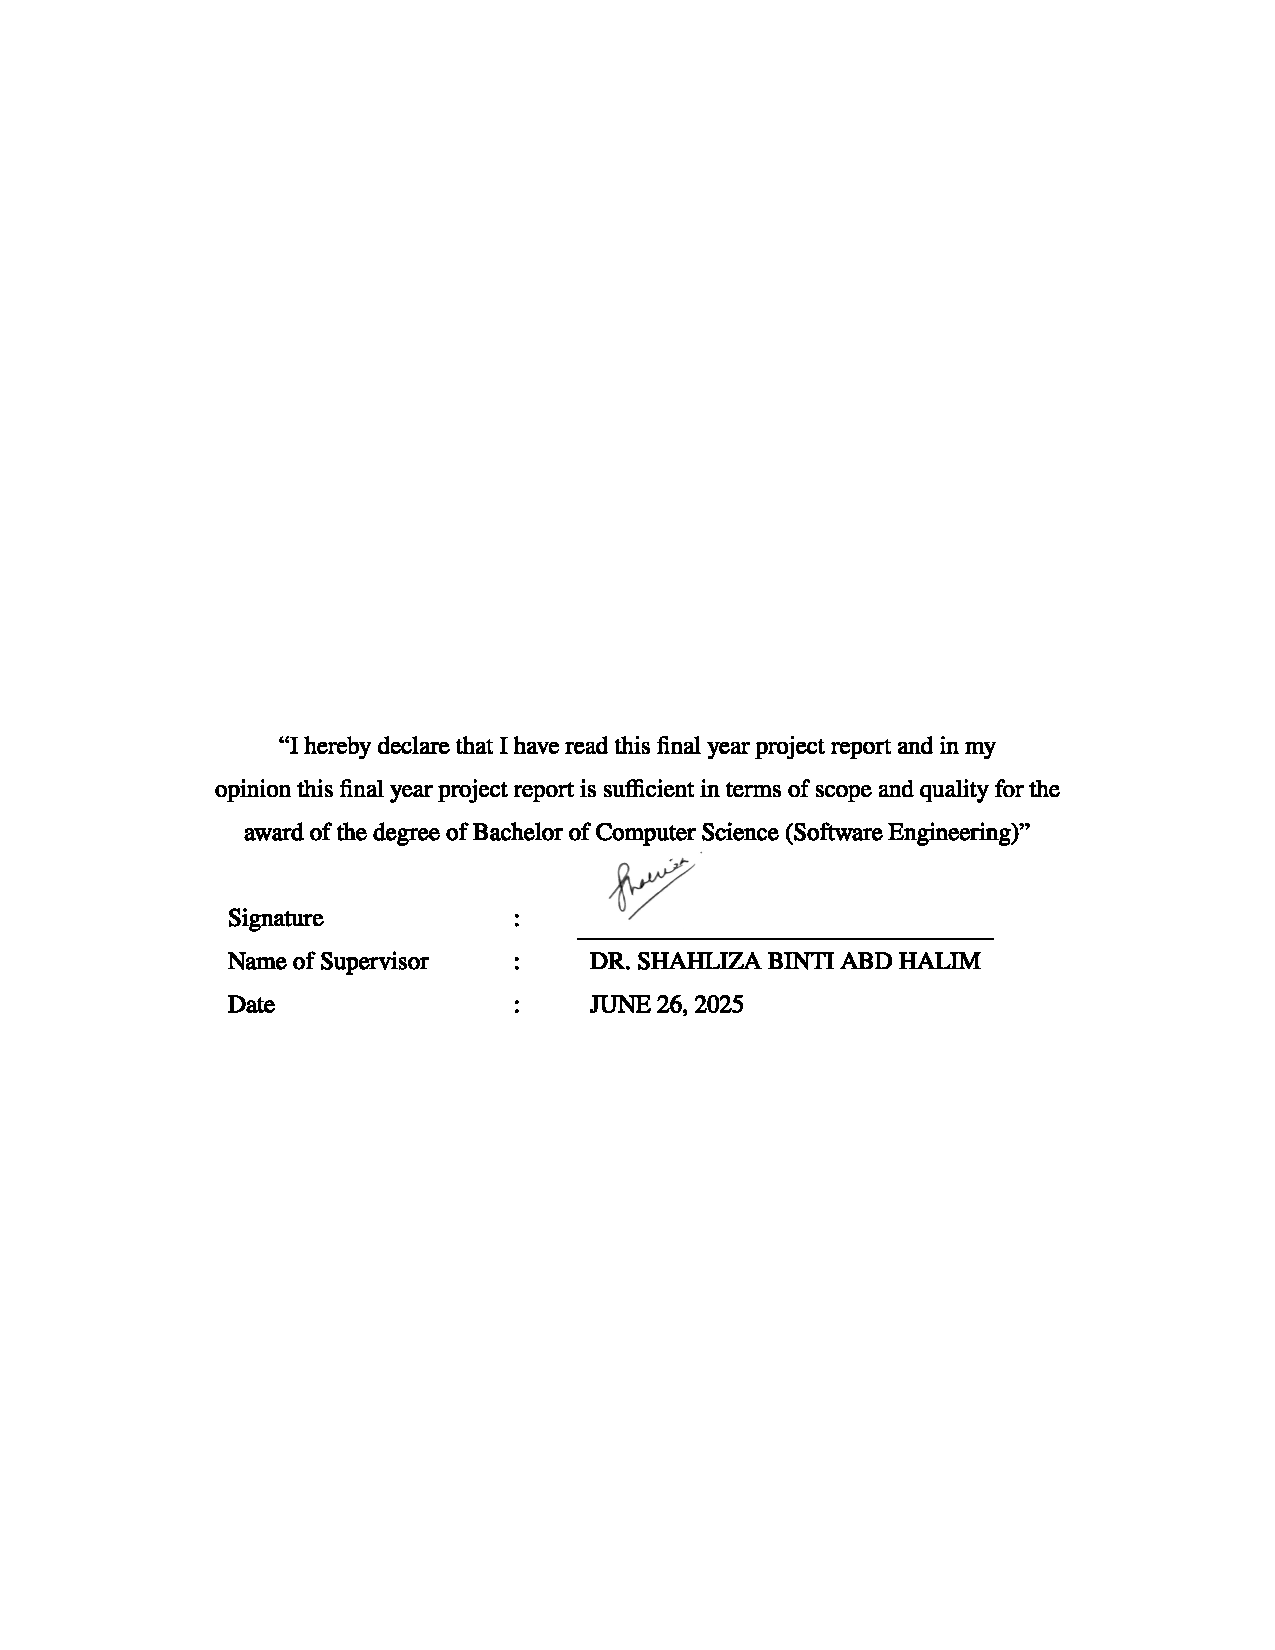
\includepdf[pages=1]{./figs/super2.pdf}
\certification

\frontmatter
\maketitle
\declaration

\normalsize
% ----------------------------------------------------------------

\begin{dedication}
    This thesis is dedicated to my father, who taught me that the best kind of knowledge to have is that which is learned for its own sake. It is also dedicated to my mother, who taught me that even the largest task can be accomplished if it is done one step at a time.\
\end{dedication}

\begin{acknowledgement}
    In preparing this thesis, I was in contact with many people, researchers, academicians, and practitioners. They have contributed towards my understanding and thoughts. In particular, I wish to express my sincere appreciation to my main thesis supervisor, Dr. Shahliza Binti Abd Halim, for encouragement, guidance, critics and friendship. Without her continued support and interest, this thesis would not have been the same as presented here.

    My fellow students should also be recognised for their support. My sincere appreciation also extends to all my colleagues and others who have provided assistance at various occasions. Their views and tips are useful indeed. Unfortunately, it is not possible to list all of them in this limited space. I am grateful to all my family members.
\end{acknowledgement}

\begin{abstract}
    LexiFlow addresses the critical challenge of making authentic Mandarin content accessible and comprehensible for language learners. Traditional methods for creating learning materials are labor-intensive, requiring manual transcription, translation, and annotation, which limits the availability of engaging resources. Existing platforms often depend on pre-existing subtitles and lack support for Mandarin-specific features such as pinyin and sentence-level segmentation. LexiFlow is a web-based platform that automates the processing of Mandarin audio and video by leveraging advanced voice activity detection, automatic speech recognition, neural machine translation, and pinyin generation. The system segments content into linguistically meaningful units, generates synchronized bilingual subtitles with pinyin, and stores processed materials in a searchable database for instant reuse. This approach reduces the workload for educators, expands the library of authentic content, and provides learners with accurate, time-aligned transcriptions and translations. LexiFlow’s modular, pipe-and filter architecture ensures scalability and maintainability, while its user-driven content model fosters personalized learning. It is hoped that the development of LexiFlow can demonstrate the feasibility and effectiveness of integrating state-of-the-art language technologies to enhance Mandarin language acquisition through real-world content.
\end{abstract}

\begin{abstrak}
    LexiFlow menangani cabaran kritikal untuk menjadikan kandungan Mandarin tulen boleh diakses dan difahami oleh pelajar bahasa. Kaedah tradisional untuk mencipta bahan pembelajaran adalah intensif buruh, memerlukan transkripsi manual, terjemahan dan anotasi, yang mengehadkan ketersediaan sumber yang menarik. Platform sedia ada selalunya bergantung pada sari kata sedia ada dan kekurangan sokongan untuk ciri khusus Mandarin seperti pinyin dan pembahagian peringkat ayat. LexiFlow ialah platform berasaskan web yang mengautomasikan pemprosesan audio dan video Mandarin dengan memanfaatkan pengesanan aktiviti suara lanjutan, pengecaman pertuturan automatik, terjemahan mesin saraf dan penjanaan pinyin. Sistem membahagikan kandungan ke dalam unit yang bermakna dari segi bahasa, menjana sari kata dwibahasa yang disegerakkan dengan pinyin dan menyimpan bahan yang diproses dalam pangkalan data yang boleh dicari untuk digunakan semula segera. Pendekatan ini mengurangkan beban kerja untuk pendidik, mengembangkan perpustakaan kandungan tulen dan menyediakan transkripsi dan terjemahan yang tepat dan selaras masa kepada pelajar. Seni bina modular, paip dan penapis LexiFlow memastikan kebolehskalaan dan kebolehselenggaraan, manakala model kandungan dipacu penggunanya memupuk pembelajaran yang diperibadikan. Diharapkan pembangunan LexiFlow dapat menunjukkan kebolehlaksanaan dan keberkesanan penyepaduan teknologi bahasa terkini untuk meningkatkan pemerolehan bahasa Mandarin melalui kandungan dunia sebenar.
\end{abstrak}

% ----------------------------------------------------------------
\tableofcontents
\listoftables
\listoffigures
% ----------------------------------------------------------------
%List of abbreviation 
\listofabbre
\addabbre{UTM}{Universiti Teknologi Malaysia}
\addabbre{NMT}{Neural Machine Translation}
\addabbre{ASR}{Automatic Speech Recognition}
\addabbre{VAD}{Voice Activity Detection}
\addabbre{HSK}{Hanyu Shuiping Kaoshi (Chinese Proficiency Test)}
\addabbre{API}{Application Programming Interface}
\addabbre{SQL}{Structured Query Language}
\addabbre{NoSQL}{Not Only SQL}

%List of symbols 
%\listofsymbols
%\addsymbol{$\gamma$}{gamma}

%Uncomment if have appendices
\listofappendices

% ----------------------------------------------------------------

\mainmatter
\chapter{Introduction}
\section{Introduction}
With over a billion speakers and a growing influence in global business, technology, and culture, Mandarin isn’t just a language—it’s a key to the future. China’s economic rise, its dominance in manufacturing and ai, and its expanding cultural footprint mean that Mandarin opens doors to career opportunities. Yet, for many learners, the language’s complexity—tonal pronunciation and intricate characters makes mastery feel impossible.

Language acquisition research shows that people learn most effectively through meaningful exposure to authentic content~\citep{krashen1985,Mayer_2009}. Authentic content here refers to real-world materials created for native speakers, such as books, movies, news articles, podcasts, and conversations, rather than simplified or artificial resources designed specifically for language learners. When learners engage with materials that interest them personally, their motivation increases and retention improves. This natural approach aligns with how children acquire their first language—through immersion rather than memorization~\citep{cychosz2021, gowenlock2024}.

Traditional methods present challenges for many students. Textbooks and classrooms tend to emphasize grammar rules instead of natural language exposure. Current apps offer translation help but struggle with Mandarin's unique difficulties. The character system creates confusion for learners since written symbols share little connection with their pronunciations. Pinyin provides pronunciation guidance but rarely appears outside educational settings.

LexiFlow solves these problems with a web platform that combines sentence segmentation with machine translation models. The system processes audio by detecting sentence boundaries and handling each segment independently. By using this approach we improve accuracy and reduce the computing resource needed. The system then maintains a database of previously processed content to eliminate duplicate processing and provide students with materials matching their interests and skill levels.
\section{Problem Background}
UTM language lecturers have observed a challenge in their students' language development. Although many students can pass written exams by studying vocabulary and grammar rules, they tend to struggle when faced with real-world Mandarin conversations. This gap between academic performance and communication skills presents a barrier to students' learning experience. Authentic content will expose students to useful vocabulary, natural speech patterns, and cultural context that textbooks simply cannot provide, especially when aligned with students' personal interests to enhance engagement.

The current approach to creating Mandarin learning content remains labor-intensive. Lecturers begin by sourcing authentic audio or video materials. Often spending considerable time searching for suitable content. Once content is selected, instructors will manually transcribe the spoken Mandarin, annotate with pinyin, and write the translation. This process can take upwards of 8 to 10 hours for only a few minutes of material and imposes a substantial burden on educators.

Existing solutions fail to address these challenges. Popular platforms like LanguageReactor depend entirely on the availability of YouTube subtitles, which is rare for Mandarin content compared to English materials. Meanwhile, general transcription services like Transcribe.com process content without the timestamped subtitle format that allows students to connect specific sounds with written text, and they lack pinyin support that Mandarin learners need for pronunciation guidance.

Students require a system that efficiently processes authentic Mandarin content while displaying spoken language alongside its written representation. This solution must provide accurate transcriptions with timestamps, pinyin pronunciation guides, and quality translations that connect naturally spoken Mandarin to its written form.
\section{Project Aim}
Develop LexiFlow, a web platform that efficiently processes, transcribes, and translates authentic Mandarin using advanced sentence-level segmentation and translation models. In order to help students understand real world mandarin conversations.
\section{Project Objectives}\label{sec:obj}
The objectives of the project are:
\begin{enumerate}[label= (\alph*)]
    \item To identify and gather requirements from primary stakeholders, including language learners and educators.
    \item To design a web-based platform with a user interface and a database that provides synchronized, time-stamped bilingual subtitles.
    \item To develop a web platform based on stakeholder requirements, adding features such as audio/video processing, transcription, translation, and pinyin generation.
    \item To test and validate the platform using testing methodologies and domain expert's feedback to ensure accuracy in transcription, translation, and subtitle synchronization.
\end{enumerate}
\section{Project Scopes}
The scopes of the project are:
\begin{enumerate}[label= (\alph*)]
    \item The proposed platform will accept long-form audio or video input (up to 120 minutes) from user-uploaded files or YouTube URLs.
    \item The proposed platform will perform voice activity detection (VAD) and end-of-sentence detection to segment audio into linguistically meaningful sentence-level chunks.
    \item The proposed platform will generate transcriptions using automatic speech recognition (ASR) and translations via Neural Machine Transformer (NMT) model.
    \item The proposed platform will produce synchronized, timestamped bilingual subtitles with original language text, target-language translation and pinyin annotations by utilizing the transformer model.
    \item The proposed platform will store processed subtitles in a searchable database indexed by content identifiers (e.g., URLs) to enable instant reuse without reprocessing.
    \item The proposed platform will provide a web interface for uploading content, customizing subtitle outputs
\end{enumerate}
\section{Project Importance}
The LexiFlow project is important because it aims to enhance the language learner’s experience. LexiFlow will overcome the problem of limited resources from online platforms and lecturers. By integrating machine translation models for translation and transcription, LexiFlow will allow students to study from content they are interested in learning from.
\section{Report Organization}
This thesis is divided into five comprehensive chapters. Chapter 1 introduces the project and outlines the background, purpose, objectives, scope, importance and structure of the report. Chapter 2 provides an in-depth literature review that examines existing systems and technologies related to speech recognition, translation models, and user interface considerations, including a comparative analysis with current market solutions.

Chapter 3 describes the system development methodology, detailing the chosen software development life cycle, the rationale for method selection, and the key stages of development. Chapter 4 focuses on requirements analysis and system design, discussing functional and non-functional requirements, database architecture, and user interface design to ensure usability and functionality.

The last chapter, Chapter 5, concludes the paper, summarizes the results, discusses the achievement of the project goals, and makes recommendations for future enhancements to extend and improve the LexiFlow system. This organizational structure ensures a clear and logical progression, facilitating detailed discussions on all aspects of the project from conceptualization to implementation and evaluation.
\chapter{LITERATURE REVIEW}
\section{Introduction}
This chapter reviews existing literature and technologies relevant to the development of the lexiflow system. It starts with an overview of second language acquisition theories that influence the design of any language learning tool. Then it highlights the challenges specific to Mandarin as a symbolic language, and examines current approaches and existing systems in the field of language learning. This literature review will provide the theoretical foundation and showcase the gaps that LexiFlow aims to address.
\section{Theories of Second Language Acquisition}
\subsection{Krashen's Input Hypothesis}
Krashen's Input Hypothesis~\citep{krashen1985} forms one of the core theoretical foundations for LexiFlow. This hypothesis asserts that language acquisition occurs when learners get exposed to comprehensible input. Here comprehensible input refers to material that is slightly above the learner's current proficiency level (i+1). In this theory, grammatical structures are acquired naturally through exposure rather than explicit instruction. This approach aligns with how children learn their first language, listening to and interacting with language in context.

Imagine a student at HSK 2 level who can handle basic conversations about daily life. According to Krashen's "i+1" principle, this learner acquires language most effectively when exposed to content at approximately HSK 3 level material that introduces new vocabulary and grammar patterns while maintaining enough familiar elements to remain comprehensible.

{Table~{\ref{tab:hsk2}}} summarizes the vocabulary requirements for each HSK (Hanyu Shuiping Kaoshi) level, which is the standardized Chinese proficiency test. As shown, each level builds cumulatively on the previous one. For example, a student at HSK 2 has mastered 300 words in total, while HSK 3 requires knowledge of 600 words.

\begin{table}[h]
    \centering
    \caption{HSK 2.0 Vocabulary Requirements \citep{hsk2}}\label{tab:hsk2}
    \begin{tabular}{@{}lll@{}}
        \toprule
        \textbf{Current Level (i)} & \textbf{Vocabulary Size} & \textbf{Cumulative Words} \\
        \midrule
        HSK 1                      & 150 words                & 150 words                 \\
        HSK 2                      & 150 words                & 300 words                 \\
        HSK 3                      & 300 words                & 600 words                 \\
        HSK 4                      & 600 words                & 1,200 words               \\
        HSK 5                      & 1,300 words              & 2,500 words               \\
        HSK 6                      & 2,500 words              & 5,000 words               \\
        \bottomrule
    \end{tabular}
    \smallskip

\end{table}

Numerous studies have validated this theory. For example,~\citet{RODRIGO2004} demonstrated that extensive exposure to comprehensible input through reading resulted in significantly greater vocabulary acquisition compared to traditional instruction methods. Similarly,~\citep{krashen2017} found that students exposed to extensive comprehensible input outperformed those following traditional grammar-translation methods, even when tested on grammatical knowledge.

However for Mandarin, the challenge lies in the ability to find authentic content that is both engaging and comprehensible. Figure~\ref{fig:mandarin_dilemma} is a perfect example of the Mandarin learning dilemma that LexiFlow aims to solve. Here we see a YouTube video which can be labeled as comprehensible input, with Chinese characters displayed as subtitles at the bottom of the screen. Crucially, these subtitles lack any Pinyin pronunciation guide, rendering them inaccessible to beginner and intermediate learners who haven't yet mastered thousands of characters. In addition, the video is not tailored to any specific proficiency level, and the subtitles option is disabled, making the use of any current translation tools impossible.

Figure~\ref{fig:mandarin_pinyin} shows an example of proper subtitles, which are hand-made by a YouTube channel. However, this process is extremely time-consuming and labor-intensive, making it very rare and with very limited library.


\begin{figure}[ht]
    \centering
    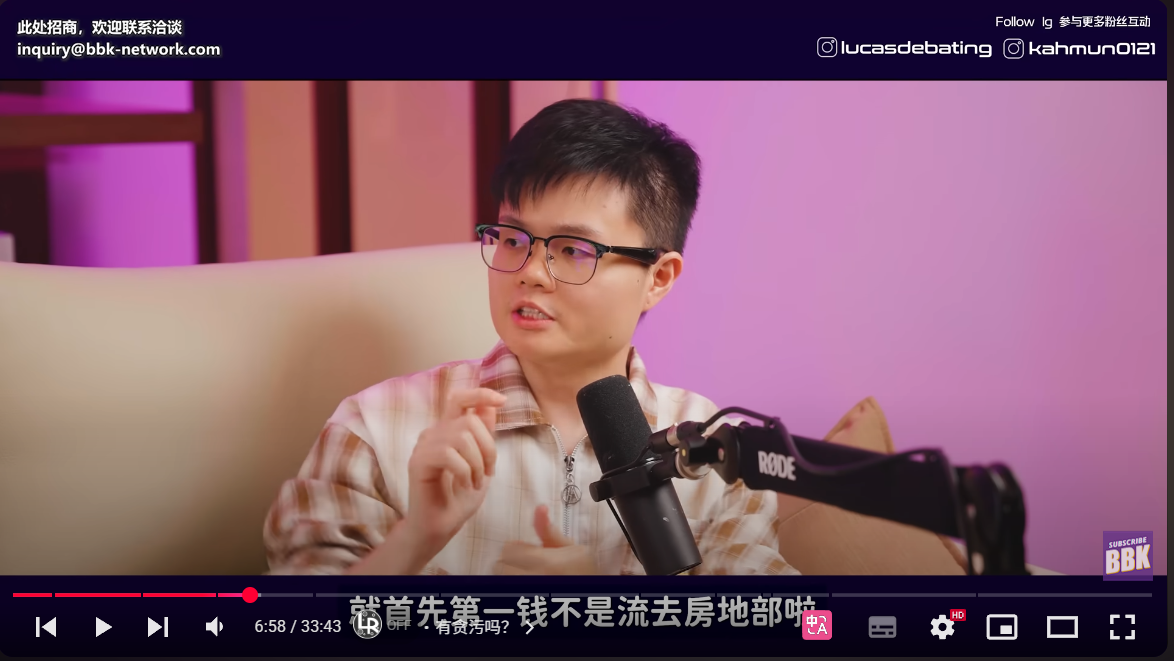
\includegraphics[width=0.8\textwidth]{./figs/yt.png}
    \caption{Example of Mandarin Learning Dilemma}
    \label{fig:mandarin_dilemma}
\end{figure}

\begin{figure}[ht]
    \centering
    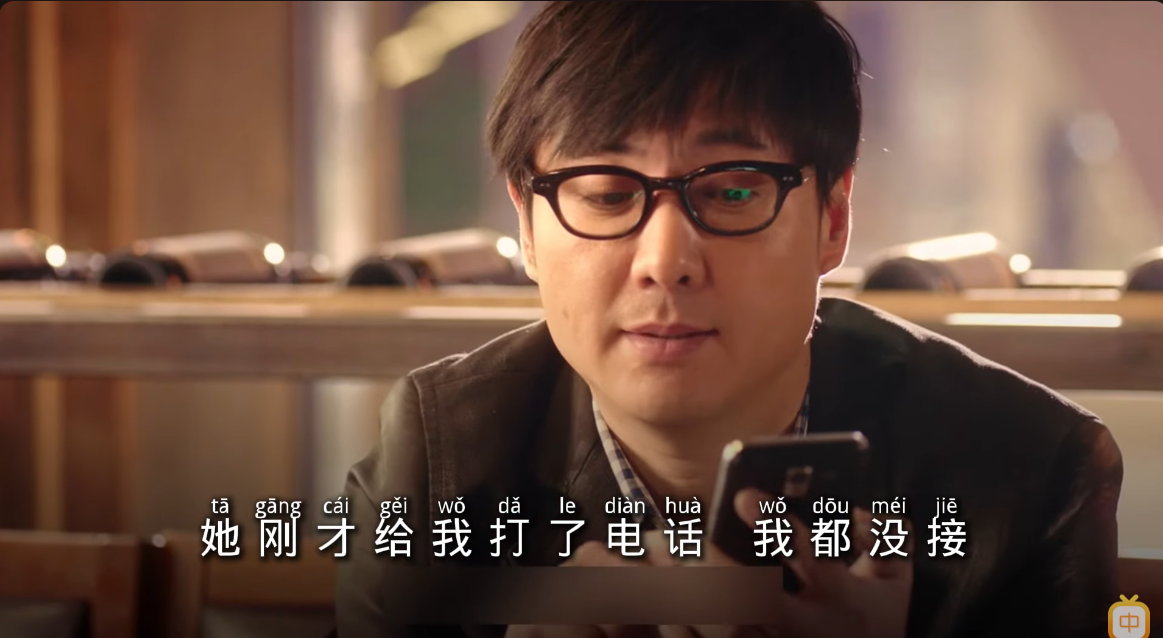
\includegraphics[width=0.8\textwidth]{./figs/yt2.png}
    \caption{Example of Proper Subtitles with Pinyin}
    \label{fig:mandarin_pinyin}
\end{figure}


\subsection{Multimedia Learning Theory}
Mayer's Multimedia Learning Theory~\citep{Mayer_2009} provides another crucial theoretical pillar for LexiFlow's approach. This theory proposes that people learn more deeply from words and pictures together than from words alone, particularly when the verbal and visual elements are presented simultaneously rather than successively.

Research by~\citet{jones2002} demonstrated that vocabulary retention increased by 42\% when learners had access to both written text and visual annotations compared to text-only learning. For character-based languages specifically,~\citet{shen2010} found that multimedia presentations that connected spoken words, written characters, and visual representations improved character recognition by 35\% compared to traditional methods.

Furthermore,~\citet{li2022} showed that Mandarin learners performed better on listening comprehension tests when they had access to subtitles during practice sessions. This shows support of LexiFlow's approach of providing multimodal input through its synchronized transcription and translation interface.
\section{Challenges of Mandarin as a Symbolic Language}
\subsection{Character Recognition and Sound Awareness}
Unlike alphabetic languages where written symbols directly represent sounds, Mandarin's logographic writing system presents new challenges for learners. Research by~\citet{everson2011} identified that Western learners require exposure to a Chinese character approximately 17 times before reliable recognition occurs, compared to just 8 exposures for alphabetic language words. This increased mental load arises from the visual complexity of the characters.

The disconnect between Mandarin's written and spoken forms creates what linguists call the `orthographic barrier'~\citep{shen2007}. This barrier significantly impedes learning efficiency, as learners struggle to connect spoken vocabulary they understand with written forms they encounter. Pinyin serves as a crucial bridge in this process, but~\citet{ye2013} found that 76\% of intermediate learners still reported difficulty transitioning from pinyin-supported texts to character-only materials.

LexiFlow addresses this challenge by maintaining the crucial connection between audio, pinyin, and characters across authentic content, allowing learners to gradually build character recognition while still accessing meaningful content through phonological representations.
\subsection{Tonal Perception and Production}
Mandarin's tonal nature presents another significant challenge identified in the literature. Research by~\citet{wang1999} demonstrated that adult learners from non-tonal language backgrounds require specialized training to accurately perceive and produce Mandarin's four tones. Their study showed that without explicit tonal training, comprehension accuracy among beginners remained below 40\% even after 200 hours of classroom instruction.

Traditional textbook approaches almost always present tones in isolation or in carefully pre-constructed dialogues. These approaches don't reflect natural speech patterns. LexiFlow creates opportunities for students to improve their tonal awareness by providing authentic content with pinyin annotations that include tone markers.
\section{Current System Analysis}
The current approach for students to study from authentic content presents significant difficulties for both learners and instructors. Based on observations at UTM and interviews with Mandarin language educators, the current process requires significant manual effort and creates limited content libraries.
\subsection{Problem with Current System}
The existing workflow for incorporating authentic Mandarin content into learning follows a highly manual, resource-intensive process that limits both quantity and quality of available materials. As illustrated in the AS-IS swimlane diagram ({Figure {\ref{fig:as_is}}}), the current process begins with either instructors or motivated students searching for potentially suitable authentic content. This search process alone is time-consuming and often yields materials that aren't appropriately matched to specific proficiency levels.

\begin{figure}[ht]
    \centering
    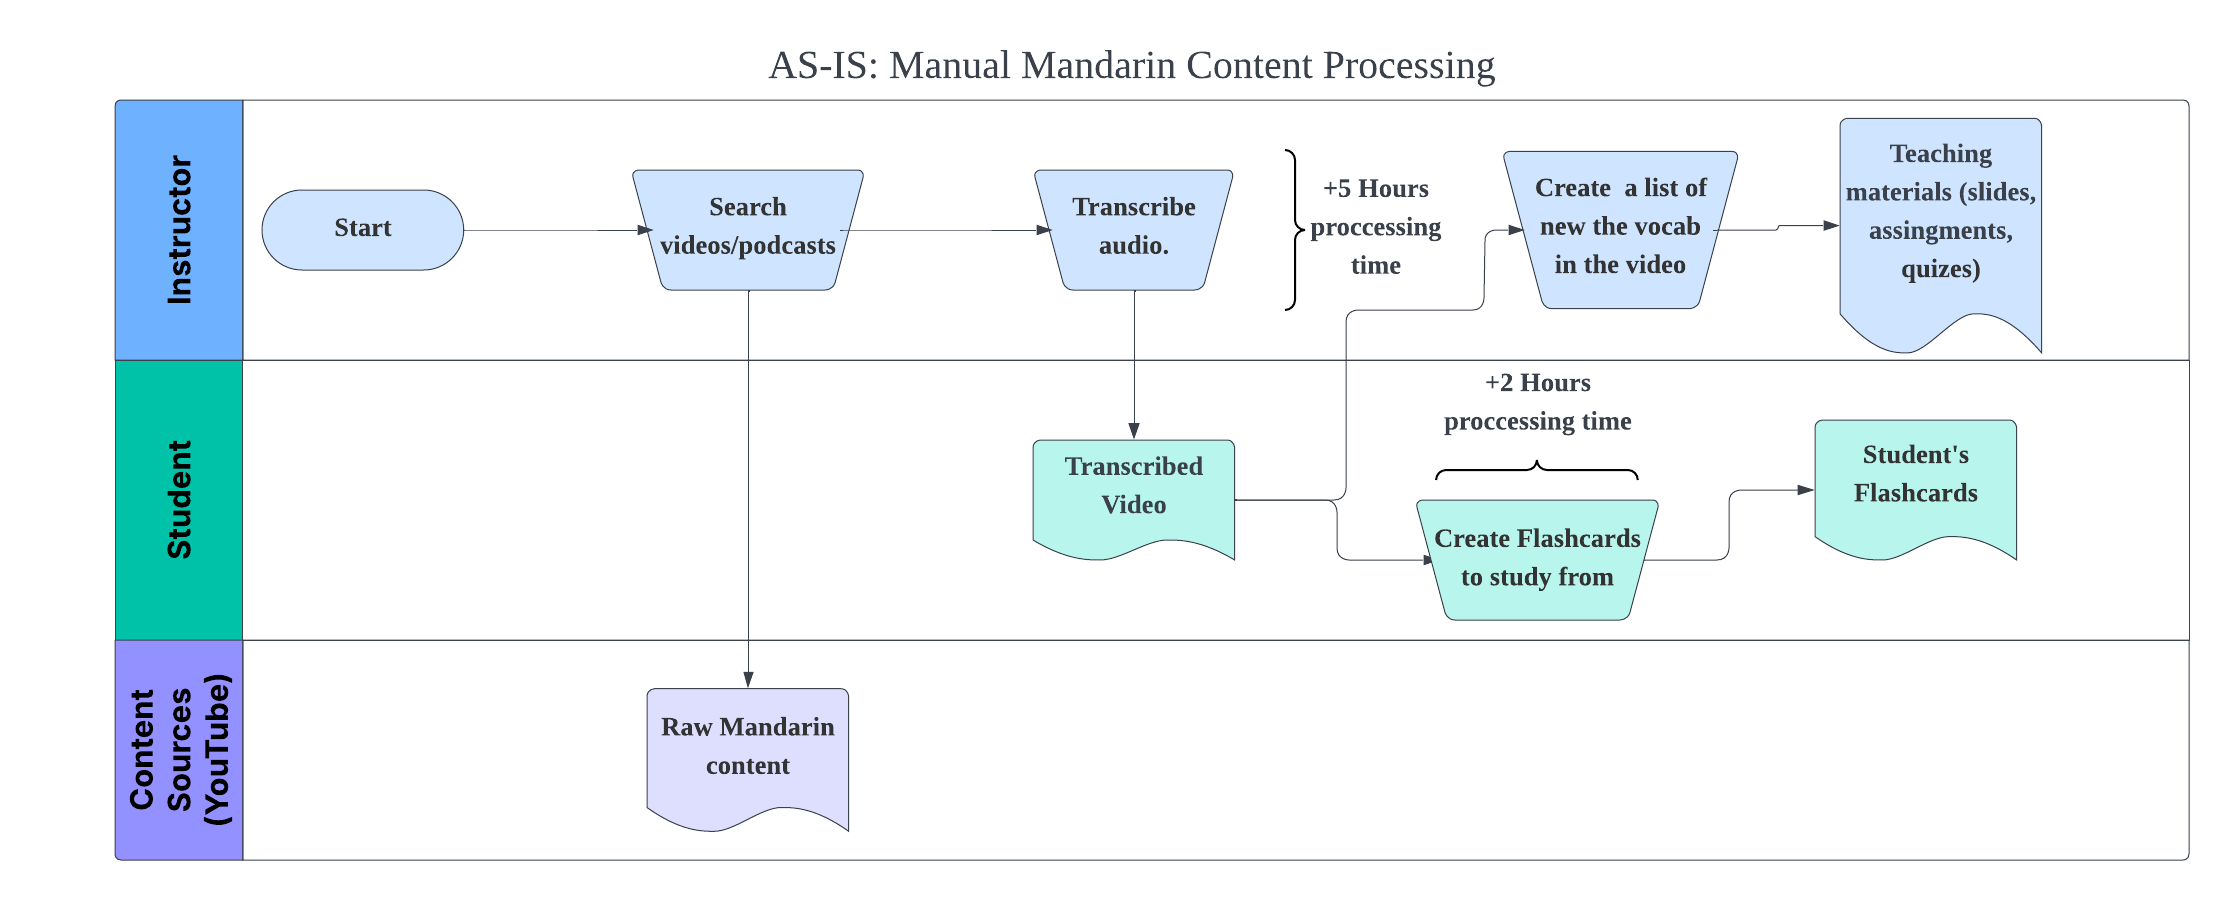
\includegraphics[width=1\textwidth]{./figs/AS-IS.PNG}
    \caption{AS-IS Swimlane Diagram}
    \label{fig:as_is}
\end{figure}

Once content is identified, the real challenges begin. Instructors must manually transcribe the Mandarin audio, create appropriate pinyin annotations, and translate content—a process that can take 8–10 hours for just a 5-minute video. This transcription burden severely limits the amount of content that can be made available to students. For students attempting this process independently, the lack of immediate feedback creates additional barriers to comprehension.

The resulting materials typically lack synchronized timestamps that would allow learners to connect spoken words with their written forms. Additionally, the content often comes without the contextual support that would make it comprehensible to learners at earlier proficiency stages, limiting its utility primarily to advanced students.
\subsection{Proposed Solution}
LexiFlow addresses these inefficiencies through a technological approach that automates the most time-consuming aspects of content processing while maintaining high quality standards. As shown in the TO-BE swimlane diagram ({Figure {\ref{fig:to_be}}}), the proposed system creates a streamlined workflow that empowers both instructors and students.

\begin{figure}[ht]
    \centering
    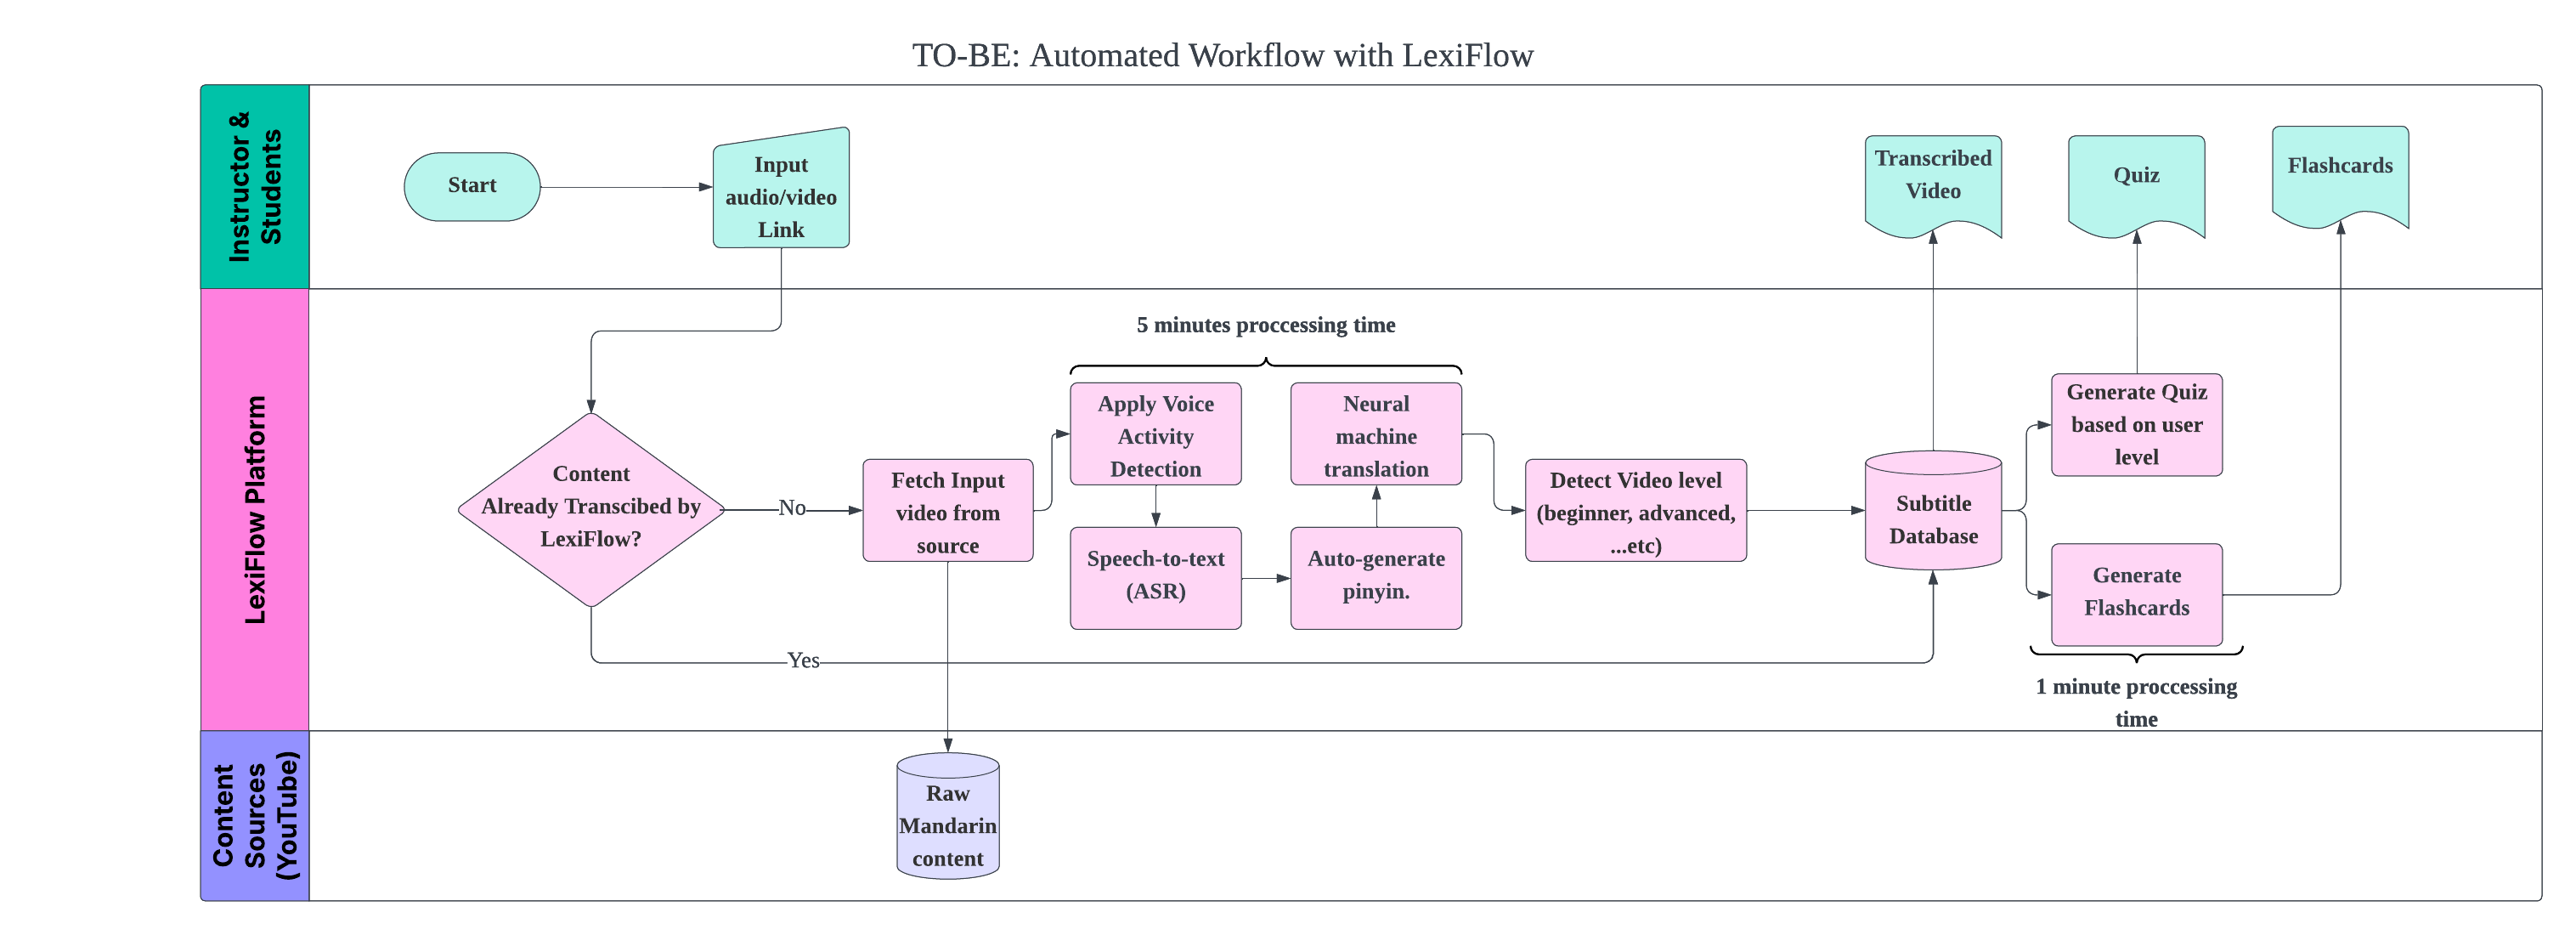
\includegraphics[width=1\textwidth]{./figs/TO-BE.PNG}
    \caption{TO-BE Swimlane Diagram}
    \label{fig:to_be}
\end{figure}


The process begins with users submitting authentic Mandarin audio or video content to the platform. LexiFlow then automatically segments the content into manageable sentence-level units using voice activation detection algorithms. Each segment is processed individually through a pipeline of automatic speech recognition (for transcription), pinyin generation, and neural machine translation (for English translation).

All processed content is stored in an indexed database, eliminating redundant processing when multiple users access the same materials. This approach creates a self-improving ecosystem where the content library grows organically based on user interests and needs.
\subsection{Comparison of Similar Video-Based Learning Platforms}
Several platforms have attempted to use video content for language learning, with varying degrees of success. FluentU, as analyzed by~\citet{xu2020}, demonstrates that carefully selected video libraries with interactive transcripts improves listening comprehension compared to traditional audio exercises. However, the study also identified content limitations as a barrier, with advanced learners complaining about insufficient variety of content. Figure~\ref{fig:fluentu-browse} shows the FluentU platform's video browse page, which highlights its curated library of videos. Figure~\ref{fig:fluentu} shows an example of a video on the FluentU platform, which includes interactive transcripts and vocabulary tools.

\begin{figure}[H]
    \centering
    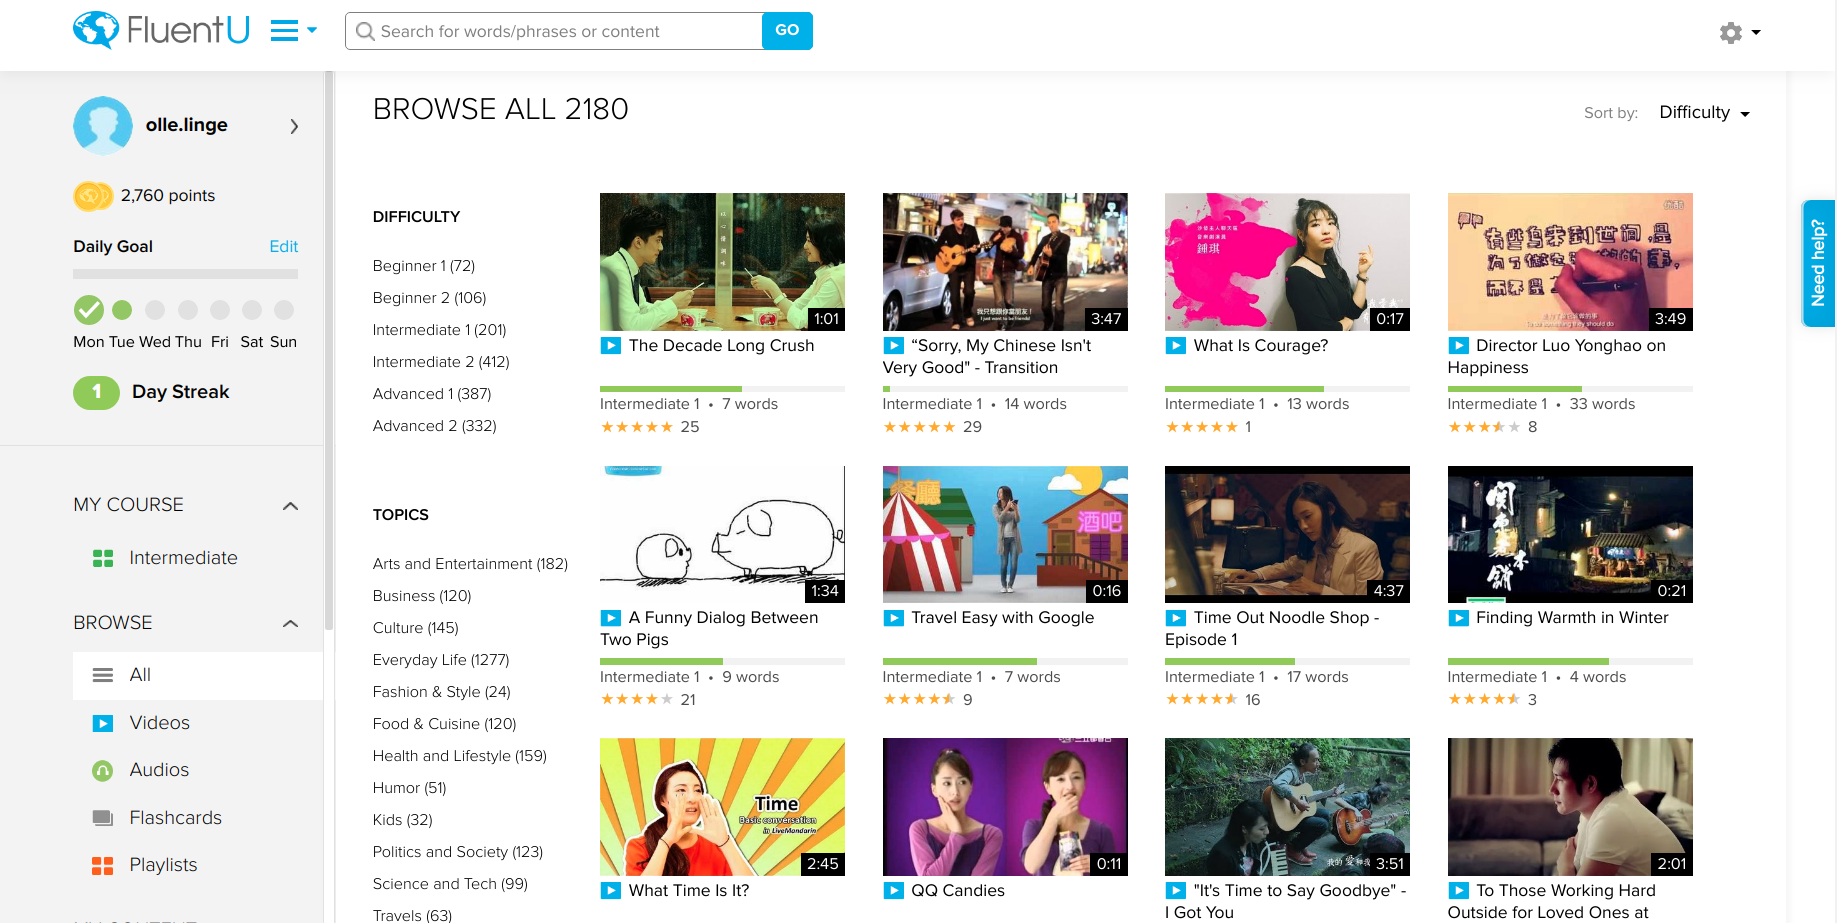
\includegraphics[width=1\textwidth]{./figs/fluentu-video-browse.png}
    \caption{FluentU Platform Video Browse Page}
    \label{fig:fluentu-browse}
\end{figure}

\begin{figure}[H]
    \centering
    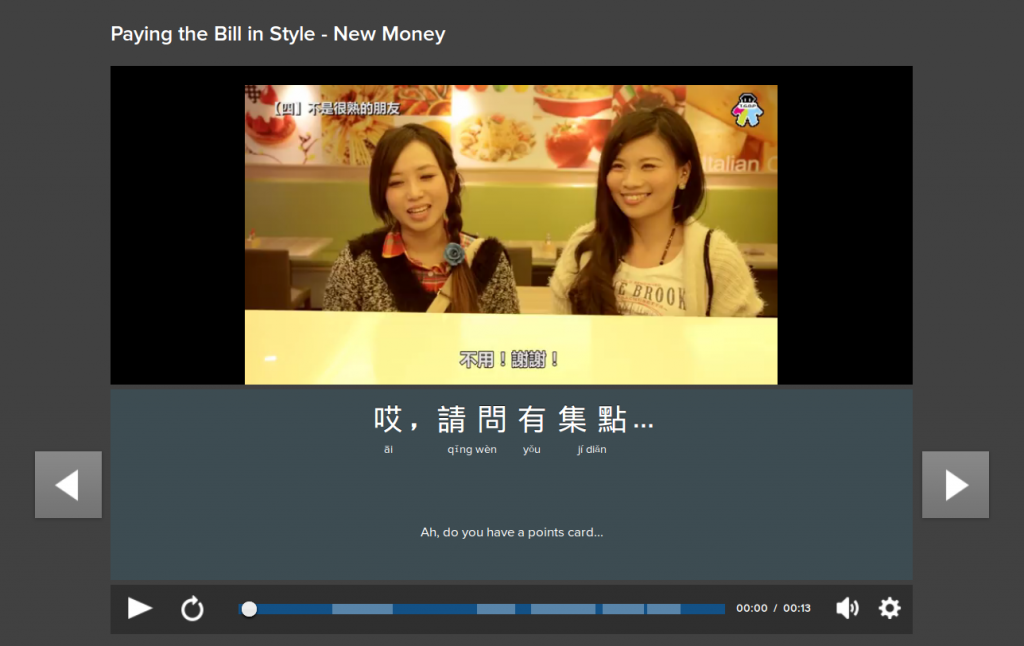
\includegraphics[width=1\textwidth]{./figs/fluentu-video.png}
    \caption{FluentU Platform Video Example}
    \label{fig:fluentu}
\end{figure}

LanguageReactor (formerly Language Learning with Netflix), as examined by~\citet{dizon2021}, is a free browser extension that allows users to overlay bilingual subtitles on Netflix and YouTube videos. It provides basic tools for vocabulary lookup and sentence by sentence playback. Unfortunately, it heavily relies on the availability of pre-existing subtitles and does not generate its own. This results in inconsistent subtitle quality. Figure \ref{fig:language-reactor-settings} shows the LanguageReactor settings page, which allows users to customize subtitle options. Figure~\ref{fig:language-reactor} shows an example of a video on the LanguageReactor platform, which includes bilingual subtitles and vocabulary tools.

\begin{figure}[H]
    \centering
    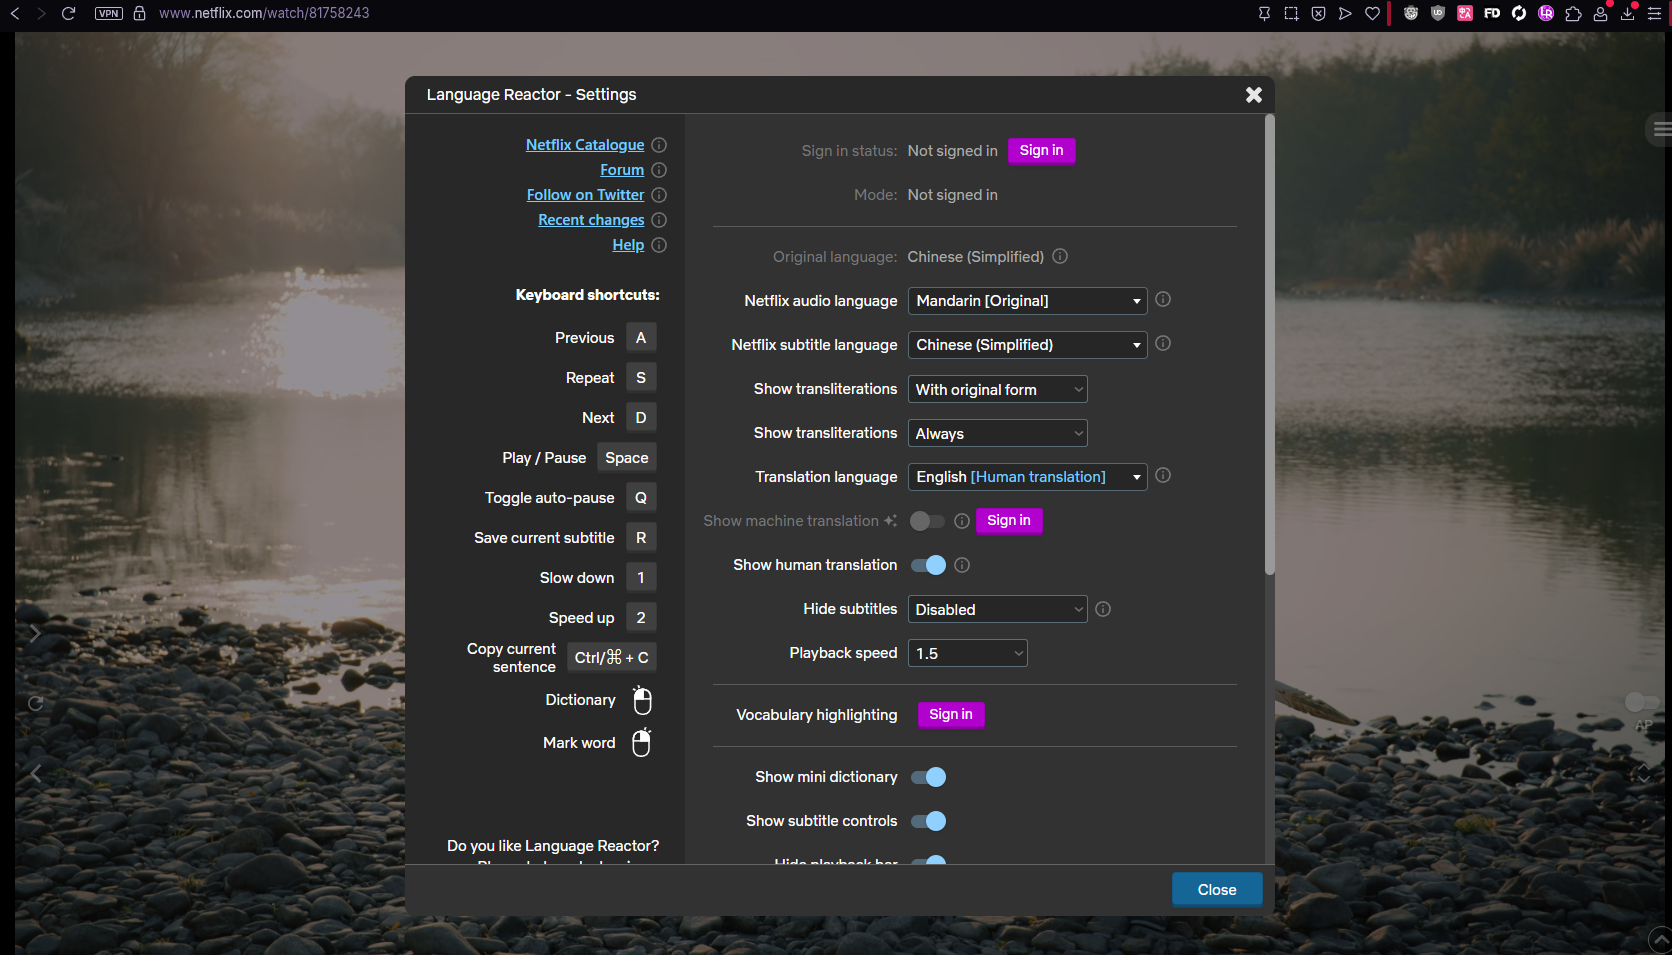
\includegraphics[width=1\textwidth]{./figs/lang_reactor-settings.png}
    \caption{LanguageReactor Settings Page From Netflix}
    \label{fig:language-reactor-settings}
\end{figure}

\begin{figure}[H]
    \centering
    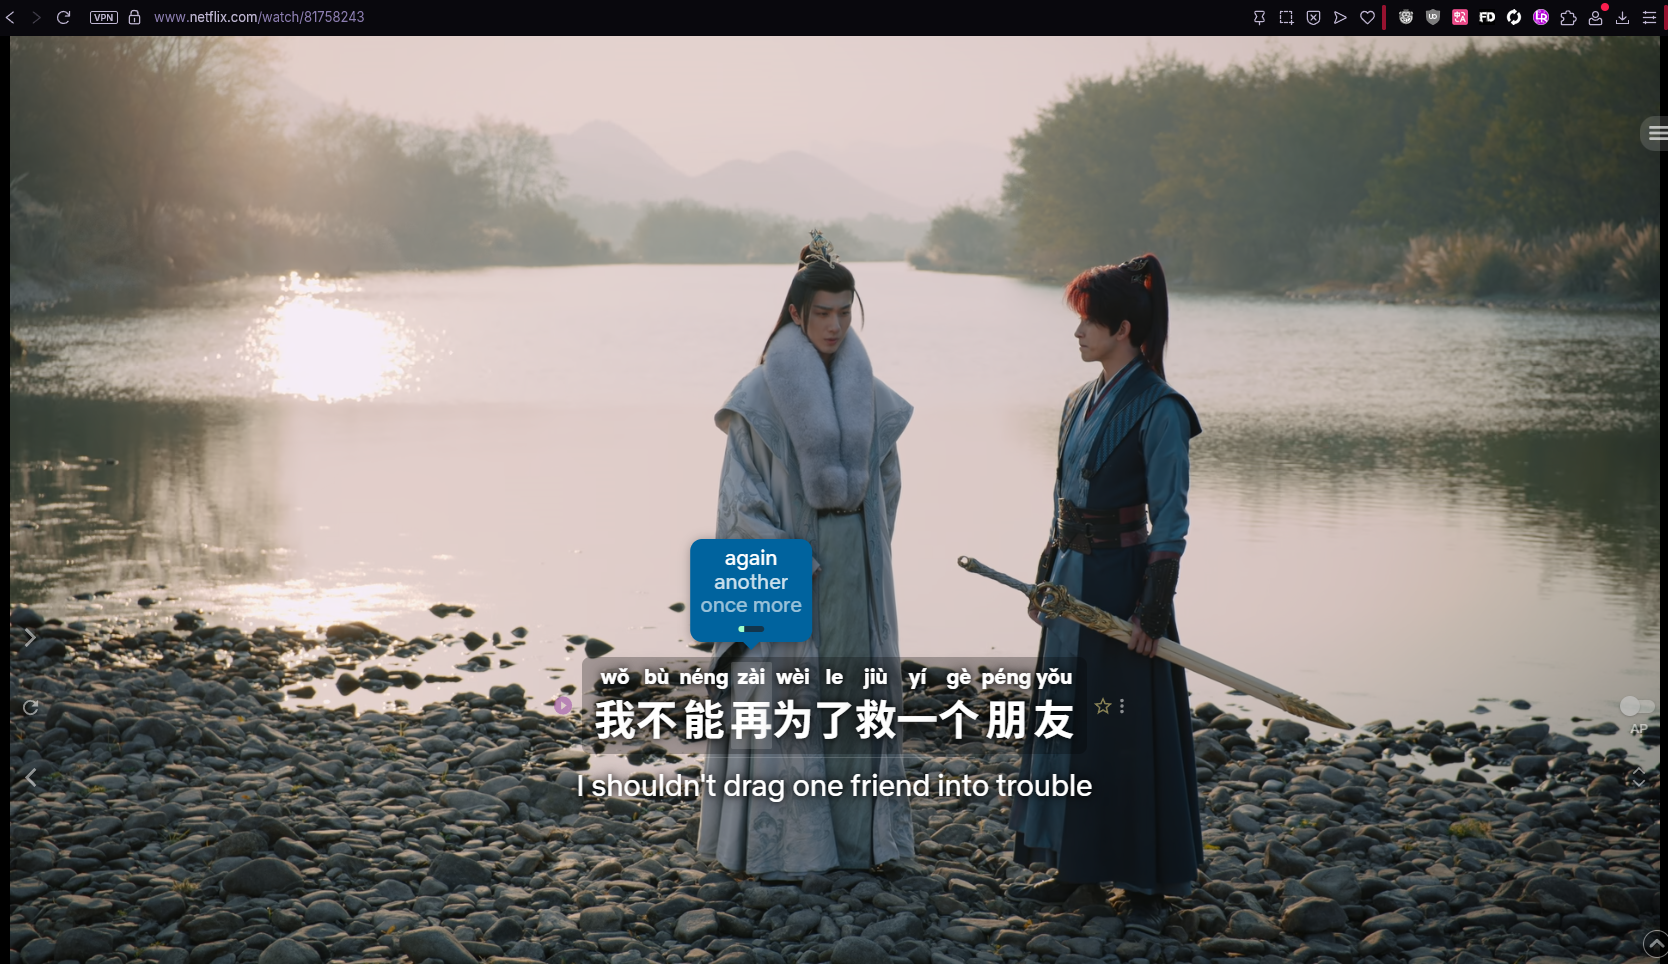
\includegraphics[width=1\textwidth]{./figs/lang_reactor.png}
    \caption{LanguageReactor Example From Netflix}
    \label{fig:language-reactor}
\end{figure}


Yabla is a subscription-based service that offers a curated video content library with interactive features. Research by~\citet{pujadas2024} demonstrated that Yabla's approach leads to better vocabulary retention compared to traditional video viewing methods. Although it provides a polished interface and well produced content, it is limited to a petite library of content that is lacking in scope and variety. However, the platform provides custom-created subtitles rather than relying entirely on third-party sources, which results in higher accuracy than LanguageReactor. Figure \ref{fig:yabla-browse} shows the Yabla platform's video browse page, which highlights its curated library of videos. Figure~\ref{fig:yabla} shows an example of a video on the Yabla platform, which includes interactive playback controls and vocabulary tools. the playback controls allow users to slow down or repeat specific segments, enhancing comprehension and retention.


\begin{figure}[H]
    \centering
    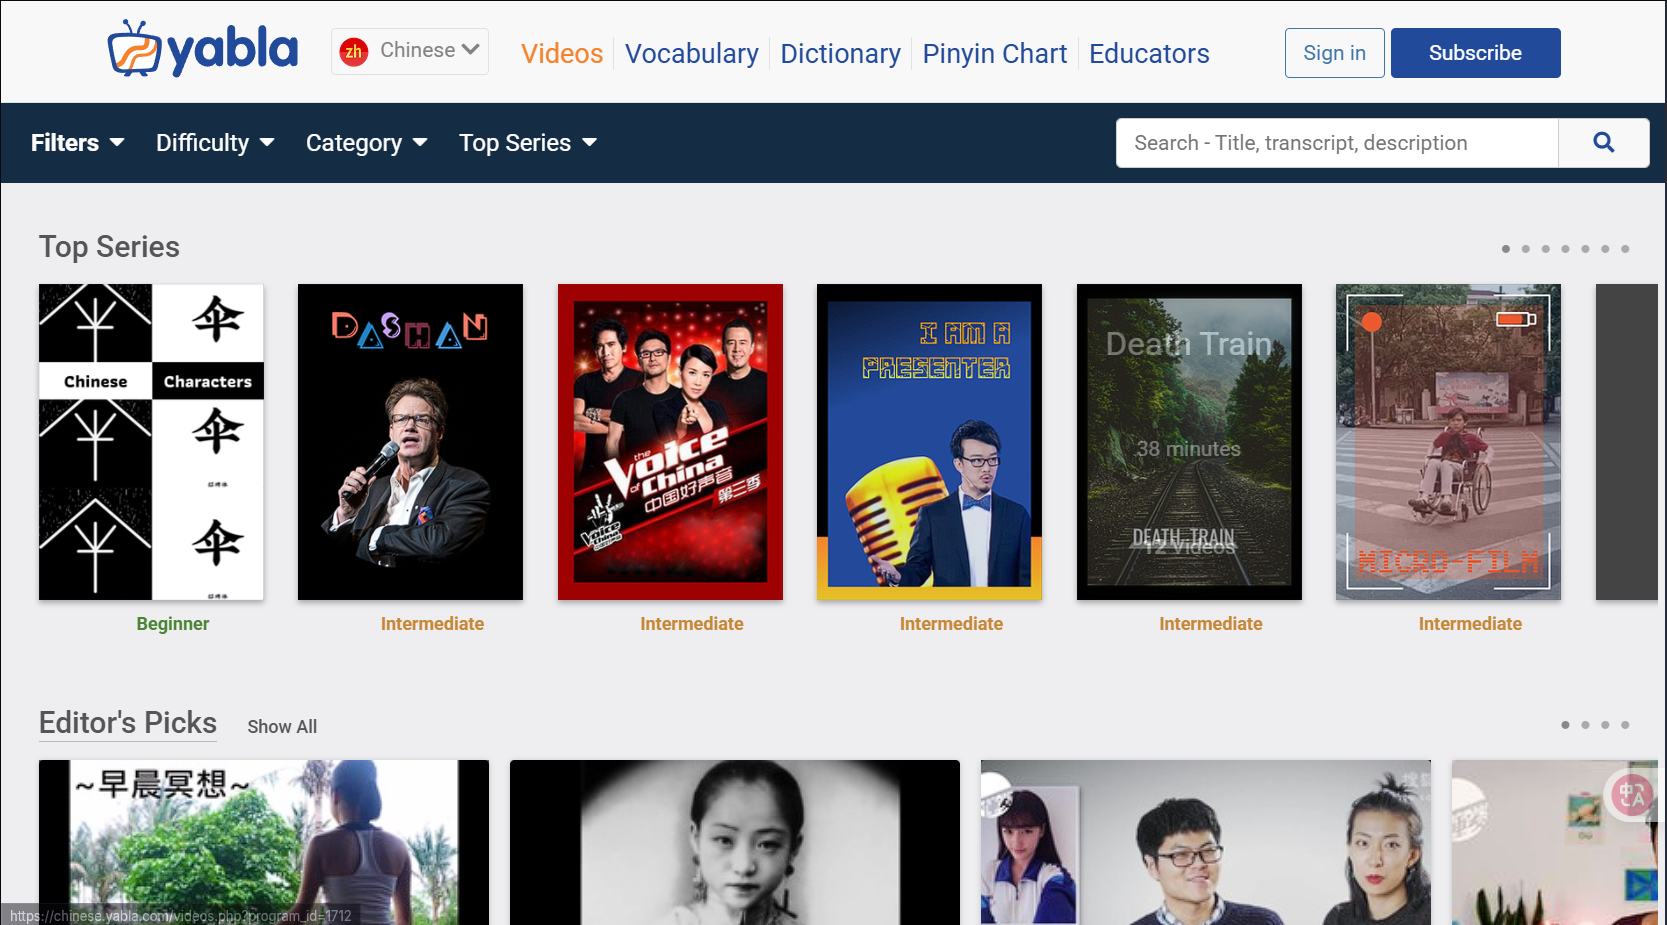
\includegraphics[width=1\textwidth]{./figs/yabla-video_browse.png}
    \caption{Yabla Platform Example}
    \label{fig:yabla-browse}
\end{figure}

\begin{figure}[H]
    \centering
    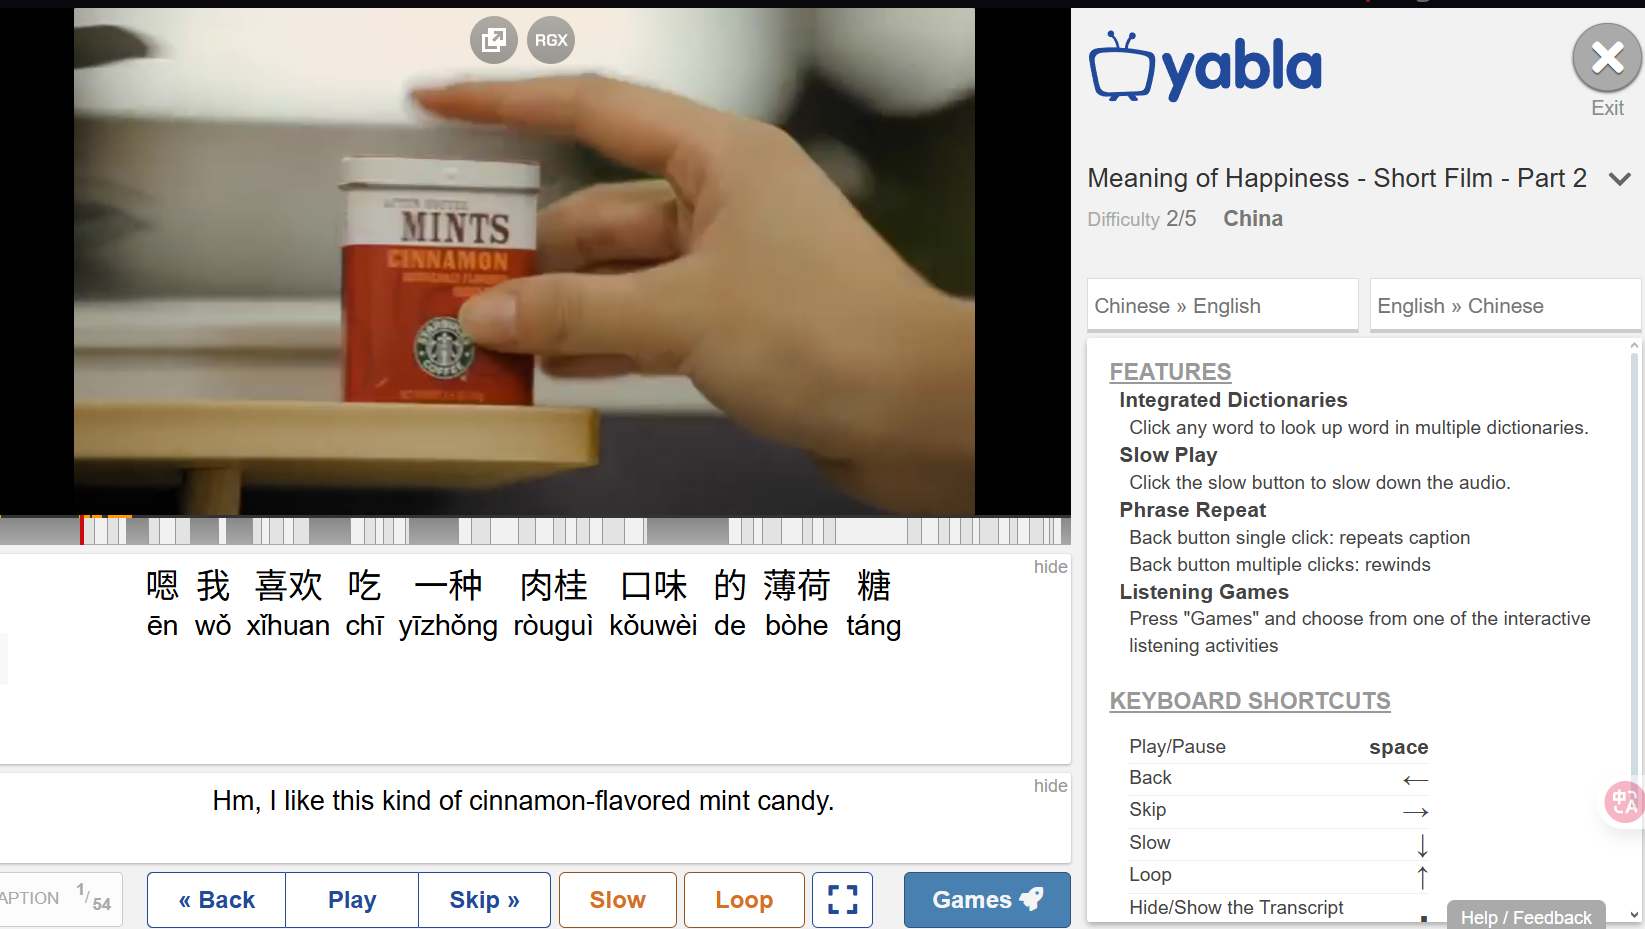
\includegraphics[width=1\textwidth]{./figs/yabla.png}
    \caption{Yabla Platform Video Example}
    \label{fig:yabla}
\end{figure}

Whilst all 3 existing systems leverage video content for language learning, they showcase different approaches to the same fundamental challenge, which is providing engaging authentic content with accurate language support. All three platforms fundamentally depend on pre-existing or manually created subtitles {as shown in table~{\ref{tab:feature_comparison}}}. This creates a content bottleneck that negatively affects Mandarin learners due to the relative shortage of subtitled content. Especially when compared to European languages like French and German.

\begin{table}[h]
    \centering
    \caption{Language Learning Platform Feature Comparison}
    \scalebox{0.85}{
        \begin{tabular}{lllll}
            \toprule
            \textbf{Feature} & \textbf{Lang.Reactor} & \textbf{FluentU} & \textbf{Yabla}    & \textbf{{LexiFlow*}}          \\
            \midrule
            Content Source   & YT/Netflix subs       & Closed library   & Curated videos    & {Any Mandarin audio}          \\
            Pinyin Support   & Word-level            & Full             & Full              & {Full}                        \\
            Processing       & Existing subs         & Manual           & Manual            & {Auto segmentation}           \\
            Growth           & Subtitle-limited      & Slow manual      & Slow manual       & {Exponential User-driven}     \\
            Efficiency       & High                  & Low              & Low               & {Medium}                      \\
            Cost             & Freemium              & Sub only         & Sub only          & {Freemium}                    \\
            Personalization  & Basic vocab           & Adaptive quiz    & Playback controls & {Interest-based} \\
            \bottomrule
        \end{tabular}
    }
    \label{tab:feature_comparison}

    \begin{flushleft}
        \small * Proposed solution
    \end{flushleft}
\end{table}

LexiFlow improves on existing platforms by offering automatic subtitle generation for any Mandarin audio or video, removing the need for pre-existing subtitles. This allows the content library to grow quickly as more users upload and process their own materials, unlike other platforms that rely on slow, manual updates. LexiFlow uses a freemium model, giving free access to core features while offering advanced tools like flashcards and personalized quizzes to premium users. It also personalizes learning by tracking user interests and saved vocabulary, then using this data to recommend relevant content and create custom study materials, making the learning experience more engaging and effective.


\section{Technologies for Video-Based Learning Platform}
\subsection{Voice Activity Detection and Sentence Segmentation}
VAD systems are essential for modern voice recognition frameworks, facilitating the detection of speech and non-speech segments on a frame-by-frame basis and triggering subsequent activities such as speech recognition, augmentation, and endpointing.~\citep{buddi2023,icassp-2019,chen2020,kumar2024}

For Mandarin specifically,~\citet{pan2025} found that using Silero-VAD~\citep{sileroVAD} model to split speech data into smaller segments improved boundary detection compared to general-purpose systems. Their research found that sentence-level segmentation yielded more accurate results than processing longer units at once. This supports LexiFlow's segment-by-segment strategy.

\subsection{Automatic Speech Recognition for Mandarin}
Automatic Speech Recognition (ASR) originated with simple systems that reacted to a limited set of sounds and has progressed into advanced systems that interact seamlessly with spoken languages. Because of the desire to automate simple tasks that require human-machine interaction, there has been increasing interest in ASR technology.~\citep{juang2005}

OpenAI's Whisper~\citep{radford2023robust} is an automatic speech recognition (ASR) system trained on 680,000 hours of multilingual and multitask supervised data collected from the web.  The Whisper architecture is a simple end-to-end approach, implemented as an encoder-decoder Transformer. This architecture is used to transcribe and identify languages with high accuracy, even in noisy or demanding audio environments.

For educational applications,~\citet{sutomo2024} discovered that even with character error rates of 6--10\%, learners stated that ASR-generated transcripts were sufficient for understanding. This finding indicates that current ASR technology has reached the point of being usable in language learning applications such as LexiFlow.
\subsection{Neural Machine Translation}
Neural Machine Translation (NMT) has significantly improved the quality and dependability of automated translation services.  According to~\citet{hassan2018}, contemporary NMT systems have achieved human parity in Chinese-English translation for news domain content, marking a significant milestone for cross-linguistic applications.

~\citet{barrault2023seamless}  SeamlessM4T v2 is Meta's cutting-edge massively multilingual and multimodal machine translation model, intended to provide high-quality, real-time translation across speech and text in nearly 100 languages.  The v2 release features the UnitY2 architecture, which includes hierarchical character-to-unit upsampling and non-autoregressive decoding.

Importantly for LexiFlow,~\citet{gary2024} showed that even when translations had small faults, showing learners both the source text and machine translations increased understanding by when compared to source-only presentation. This result demonstrates that LexiFlow's strategy of offering translations in addition to the original Mandarin content works well.

\subsection{NoSQL Database Implementation}
Modern video-based learning platforms benefit significantly from NoSQL databases due to their flexibility, scalability, and performance advantages over traditional relational databases. Unlike structured SQL databases, NoSQL systems allow for schema-less data storage, making them well-suited for handling diverse and evolving content types, such as video metadata, user interactions, and dynamic learning analytics.

NoSQL databases, particularly document-oriented stores like MongoDB, efficiently manage unstructured and semi-structured data, enabling seamless storage and retrieval of multimedia content, user profiles, and session logs. Their distributed architecture ensures high availability and horizontal scalability, which is crucial for platforms experiencing rapid growth in users and content volume. Additionally, key-value and wide-column NoSQL databases optimize read and write performance for real-time analytics, while graph databases can effectively model relationships between concepts, users, and learning materials.
\section{Summary}
This literature review has established several key findings that inform LexiFlow's development. First, it was established that Krashen's Input Hypothesis and Multimedia Learning Theory provide strong theoretical foundations for LexiFlow's approach. After that, the Mandarin's symbolic writing system and its unique challenges was discussed. Furthermore, the current language learning applications and their limitations were carefully examined. Finally, This literature review was concluded by the recent advancements in Voice Activity Detection, Automatic Speech Recognition, and Neural Machine Translation and the discussion about the models which are planned to be used in the system.
% \begin{enumerate}[label= (\alph*)]
%     \item Krashen's Input Hypothesis and Multimedia Learning Theory provide strong theoretical foundations for LexiFlow's approach of making authentic content comprehensible through technological scaffolding.
%     \item Mandarin's logographic writing system creates unique challenges that require specialized technological solutions connecting spoken and written forms.
%     \item Current language learning applications demonstrate the value of authentic video content but suffer from critical limitations in content availability and flexibility.
%     \item Recent advances in Voice Activity Detection, Automatic Speech Recognition, and Neural Machine Translation have reached sufficient maturity to support educational applications with high accuracy.
%     \item Sentence-level processing approaches offer significant advantages in both computational efficiency and accuracy compared to whole-file processing.
%     \item Interest-driven learning consistently demonstrates superior engagement and outcomes compared to prescribed content approaches.
% \end{enumerate}
This review establishes both the need for and the feasibility of LexiFlow's approach to Mandarin language learning through efficient processing of authentic content. The next chapter will detail the methodological approach to implementing these insights in the LexiFlow system.

\chapter{SYSTEM DEVELOPMENT METHODOLOGY}
\section{Introduction}
This chapter outlines the methodology used in the development of LexiFlow to ensure the successful implementation of the system. The chapter opens with the explanation as to why the hybrid Agile model was selected and why it is appropriate to adopt elements from both Agile and traditional project management approaches to achieve a balance between flexibility and structure by keeping fixed development milestones in mind. Therefore, each phase of the adopted methodology will be elaborately discussed, which in effect will give an overall comprehensive framework that guides the development of the project from initial requirements gathering to the final stage of testing and deployment of the system.

The methodology section gives a more elaborate explanation as to how the
technologies chosen for our project would fit the features of the selected technologies within the Agile processes and aligns with the LexiFlow system itself. With this, the technology stack would support the functionality of the application.

\section{Methodology Choice and Justification}
The hybrid Agile model was chosen for LexiFlow's development due to its flexibility in adapting to changing requirements while maintaining structured milestones. This method enables iterative development, which allows continuous feedback and refinement throughout the project's lifecycle. The Agile methodology is particularly well-suited for software projects where user needs may evolve, as it emphasizes collaboration, customer involvement, and responsiveness to change.

Implementing Scrum may lead to improved communication, cooperation, and software product quality, as stated by~\citet{scrum}.  Meanwhile, Waterfall's advantages include the arrangement of the phases in order to assist new developers in fully grasping the `big picture`of managing a software project across its development life cycle.  This also allows for a more in-depth grasp of the requirements, code logic, and software testing.

Each phase of the development process will be guided by Agile principles, including regular sprints, user stories, and continuous integration. This approach allows for rapid prototyping and testing of features, ensuring that the final product meets user needs effectively. {As figure {\ref{fig:methodology_overview}} shows}, the project will also incorporate traditional project management practices, such as detailed planning and documentation, to ensure that all aspects of the system are thoroughly addressed.

\begin{figure}[ht]
    \centering
    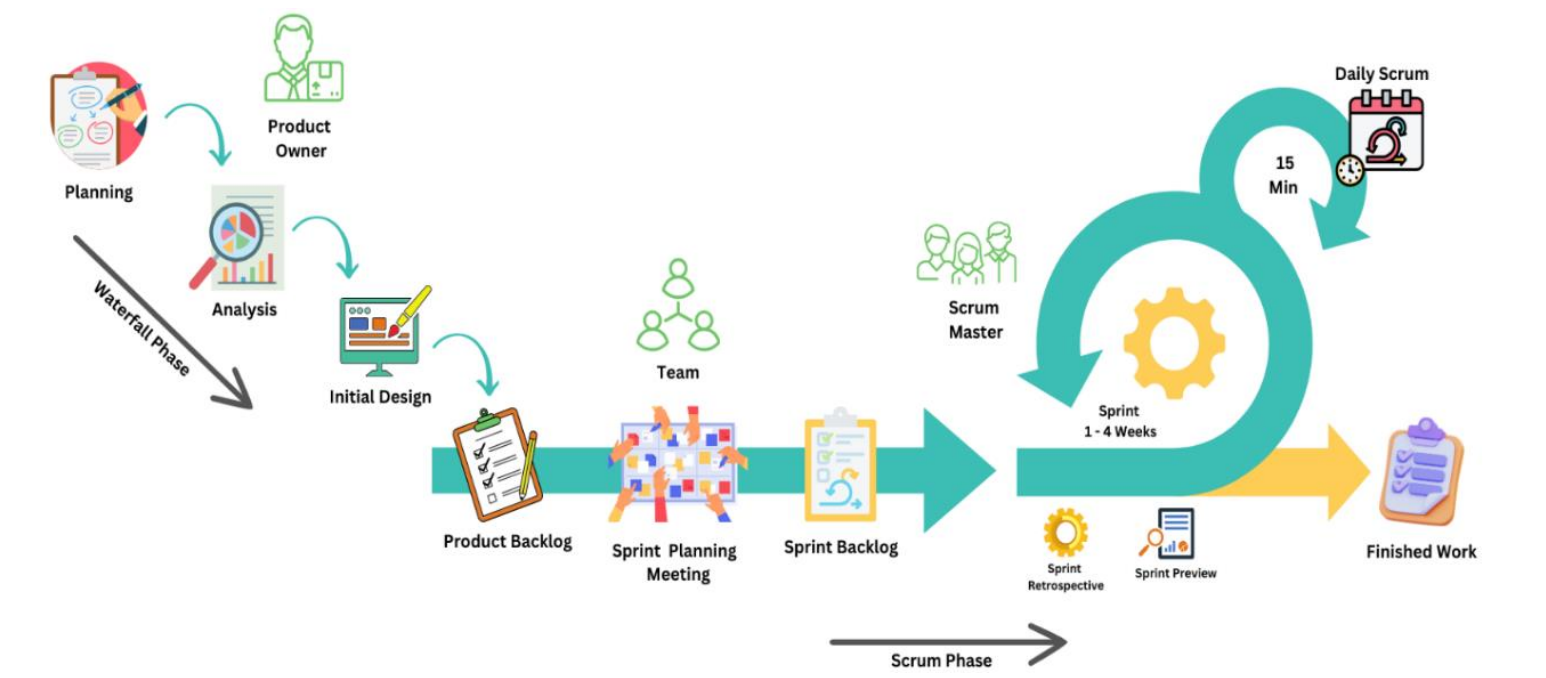
\includegraphics[width=1\textwidth]{./figs/scrum2.png}
    \caption{Hybrid-Scrum Methodology Overview~\citep{scrum2}}
    \smallskip
    \label{fig:methodology_overview}
\end{figure}

\section{Methodology Phases}

The development of LexiFlow will follow a hybrid methodology consisting of several key phases:
\begin{enumerate}[label= (\alph*)]
    \item \textbf{Planning (Waterfall):} This phase lays the groundwork for the entire project. It consists of preliminary project scoping, time estimations, resource assignment, and the determination of key stakeholders. The planning process is based on a traditional Waterfall approach, where the entire roadmap is planned in advance to provide a clear direction of the project at the beginning.

    \item \textbf{Analysis (Waterfall):} This is the phase in which every project requirement will be carefully derived and documented using a waterfall method of development. The process engages all stakeholders: language learners and lecturers in a comprehensive interview or survey to ensure there is thorough attempt at defining every functional and non-functional requirement.

    \item \textbf{Initial Design (Waterfall):} Once the requirements have been set, the project will transition immediately into design phase with the Waterfall method. This step builds a high-level plan of the entire system, and this defines the interaction of each component with other components through its interfaces. By ensuring that the design is very much in line with the user requirements, we ensure that each element of the system is clearly defined and good to go into development.

    \item \textbf{Actual Sprints (Agile):} The development will span across six sprints:
          \begin{enumerate}[label= (\roman*)]
              \item \textit{Sprint 1 – Prototype Sprint:} An initial prototype covering core functionalities is developed to validate early design assumptions, gather feedback and test the chosen models' performance.

              \item \textit{Sprint 2 – User Module:} This sprint focuses on implementing user registration, login, and profile management. It enables both students and lecturers to create and manage their accounts and learning preferences.

              \item \textit{Sprint 3 – Content Processing Module:} During this sprint, the local media uploading and YouTube URL submission functionality is built. The content will be processed by the system and produce synchronized subtitles in Mandarin, pinyin, and English translation.

              \item \textit{Sprint 4 – Interactive Learning Module:} This sprint covers vocabulary learning features such as word search, saving vocabulary, bookmarking video segments, and reporting translation errors to enhance content accuracy.

              \item \textit{Sprint 5 – Assessment Module:} This sprint implements the review and testing features. It includes generating flashcards from saved vocabulary and auto-generating quizzes based on the user’s learning history.

              \item \textit{Sprint 6 – Deployment Sprint:} Final integration and testing of all modules are conducted in this sprint. The system is deployed to the live environment with final checks, performance optimizations, and documentation.
          \end{enumerate}

    \item \textbf{Burn Down Chart (Agile):} During each sprint, a burn down chart is maintained to track remaining work against time. This visual tool helps the team monitor progress daily, quickly identify any bottlenecks, and ensure that the sprint is on track to meet its goals. It also serves as a key reference during the Sprint Review.

    \item \textbf{Sprint Review (Agile):} At the end of each sprint, a review session is held to demonstrate the new features to stakeholders. Their feedback is collected and used to refine upcoming sprint goals, ensuring continuous alignment with user expectations.

    \item \textbf{Sprint Retrospective (Agile):} Following every sprint review, the team conducts a retrospective to assess what went well, what didn’t, and how processes can be improved in the next sprint. This promotes continuous improvement and team collaboration.

    \item \textbf{Maintenance (Agile):} Once deployed, the system enters the maintenance phase. Using Agile practices, updates and enhancements will be delivered in iterative cycles to address bugs, respond to user feedback, and introduce new features, ensuring the product remains robust and user-centric over time.
\end{enumerate}

Gannt chart in Figure~\ref{fig:jira} shows the timeline of the FYP 1 and the prototype sprint while Figure~\ref{fig:jira2} shows the timeline of FYP 2. The Gannt chart is created using Jira, which is a project management tool that helps to track the progress of the project and manage the tasks effectively.


\begin{figure}[H]
    \centering
    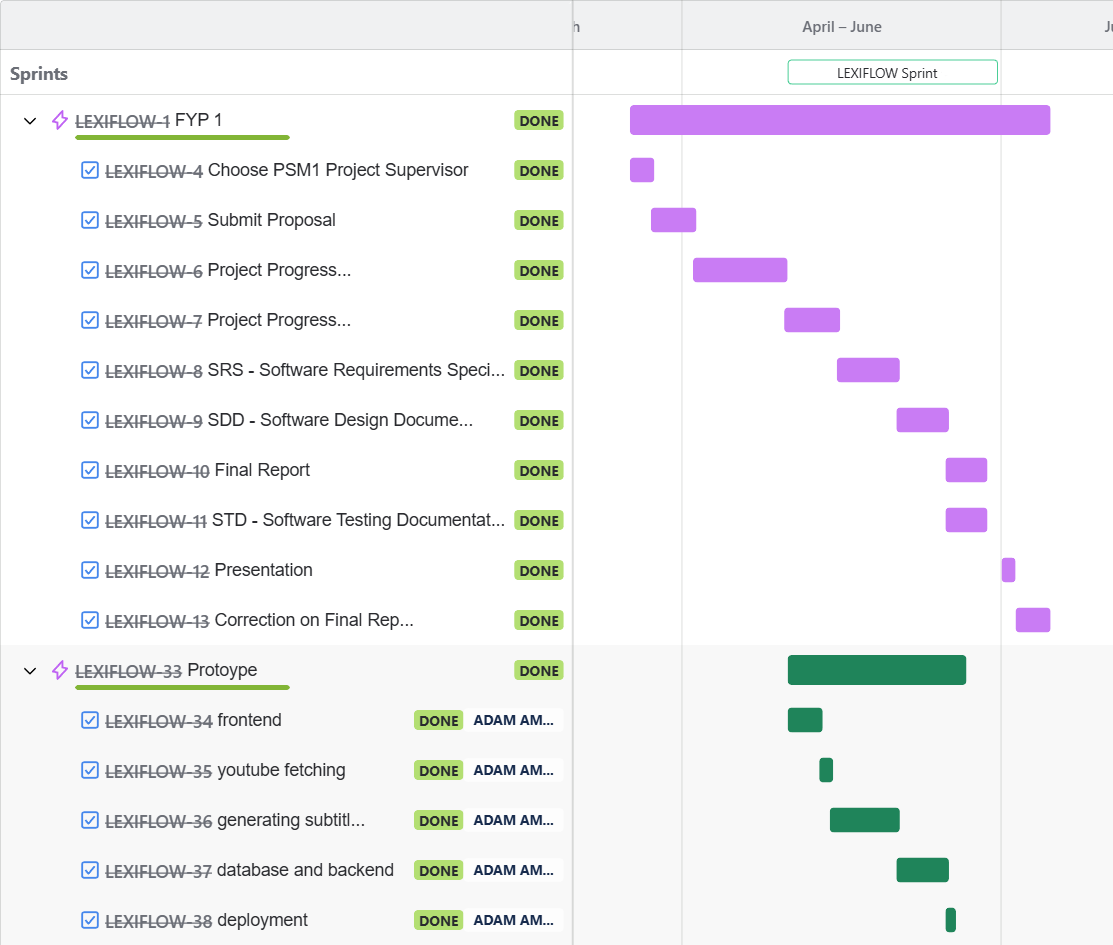
\includegraphics[width=0.75\textwidth]{./figs/fyp1_gantt.png}
    \caption{Gantt Chart FYP1}\label{fig:jira}
\end{figure}

\begin{figure}[H]
    \centering
    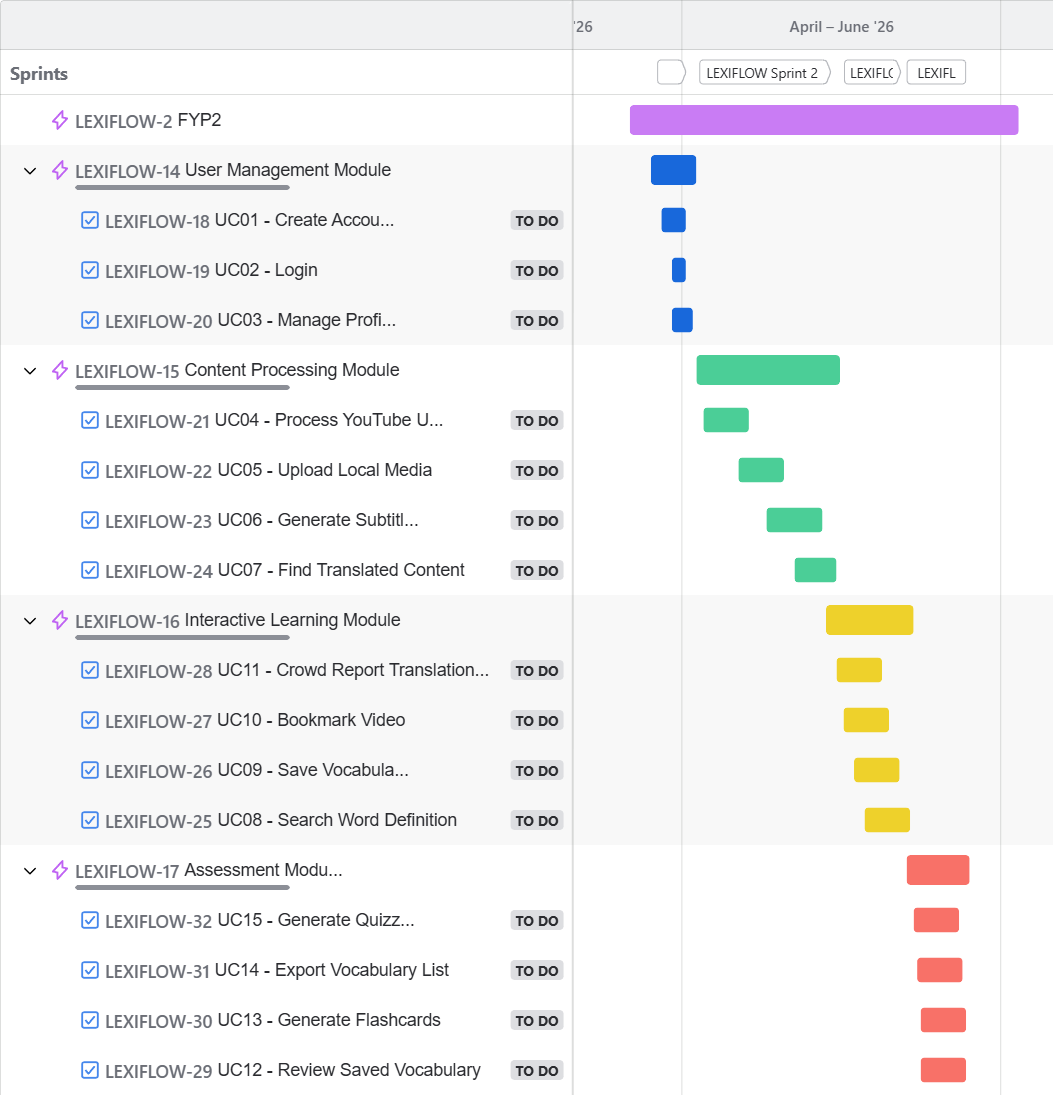
\includegraphics[width=0.75\textwidth]{./figs/fyp2_gantt.png}
    \caption{Gantt Chart FYP2}\label{fig:jira2}
\end{figure}

The first sprint is the prototype sprint, which is already completed. The burn down chart is shown in Figure~\ref{fig:burndown}. The burn down chart shows the progress of the project and the remaining tasks to be completed. Also, the sprint review with the stakeholders is completed. The feedback from the stakeholder is shown in Appendix~\ref{app:feedback-on-prototype}. 

\begin{figure}[H]
    \centering
    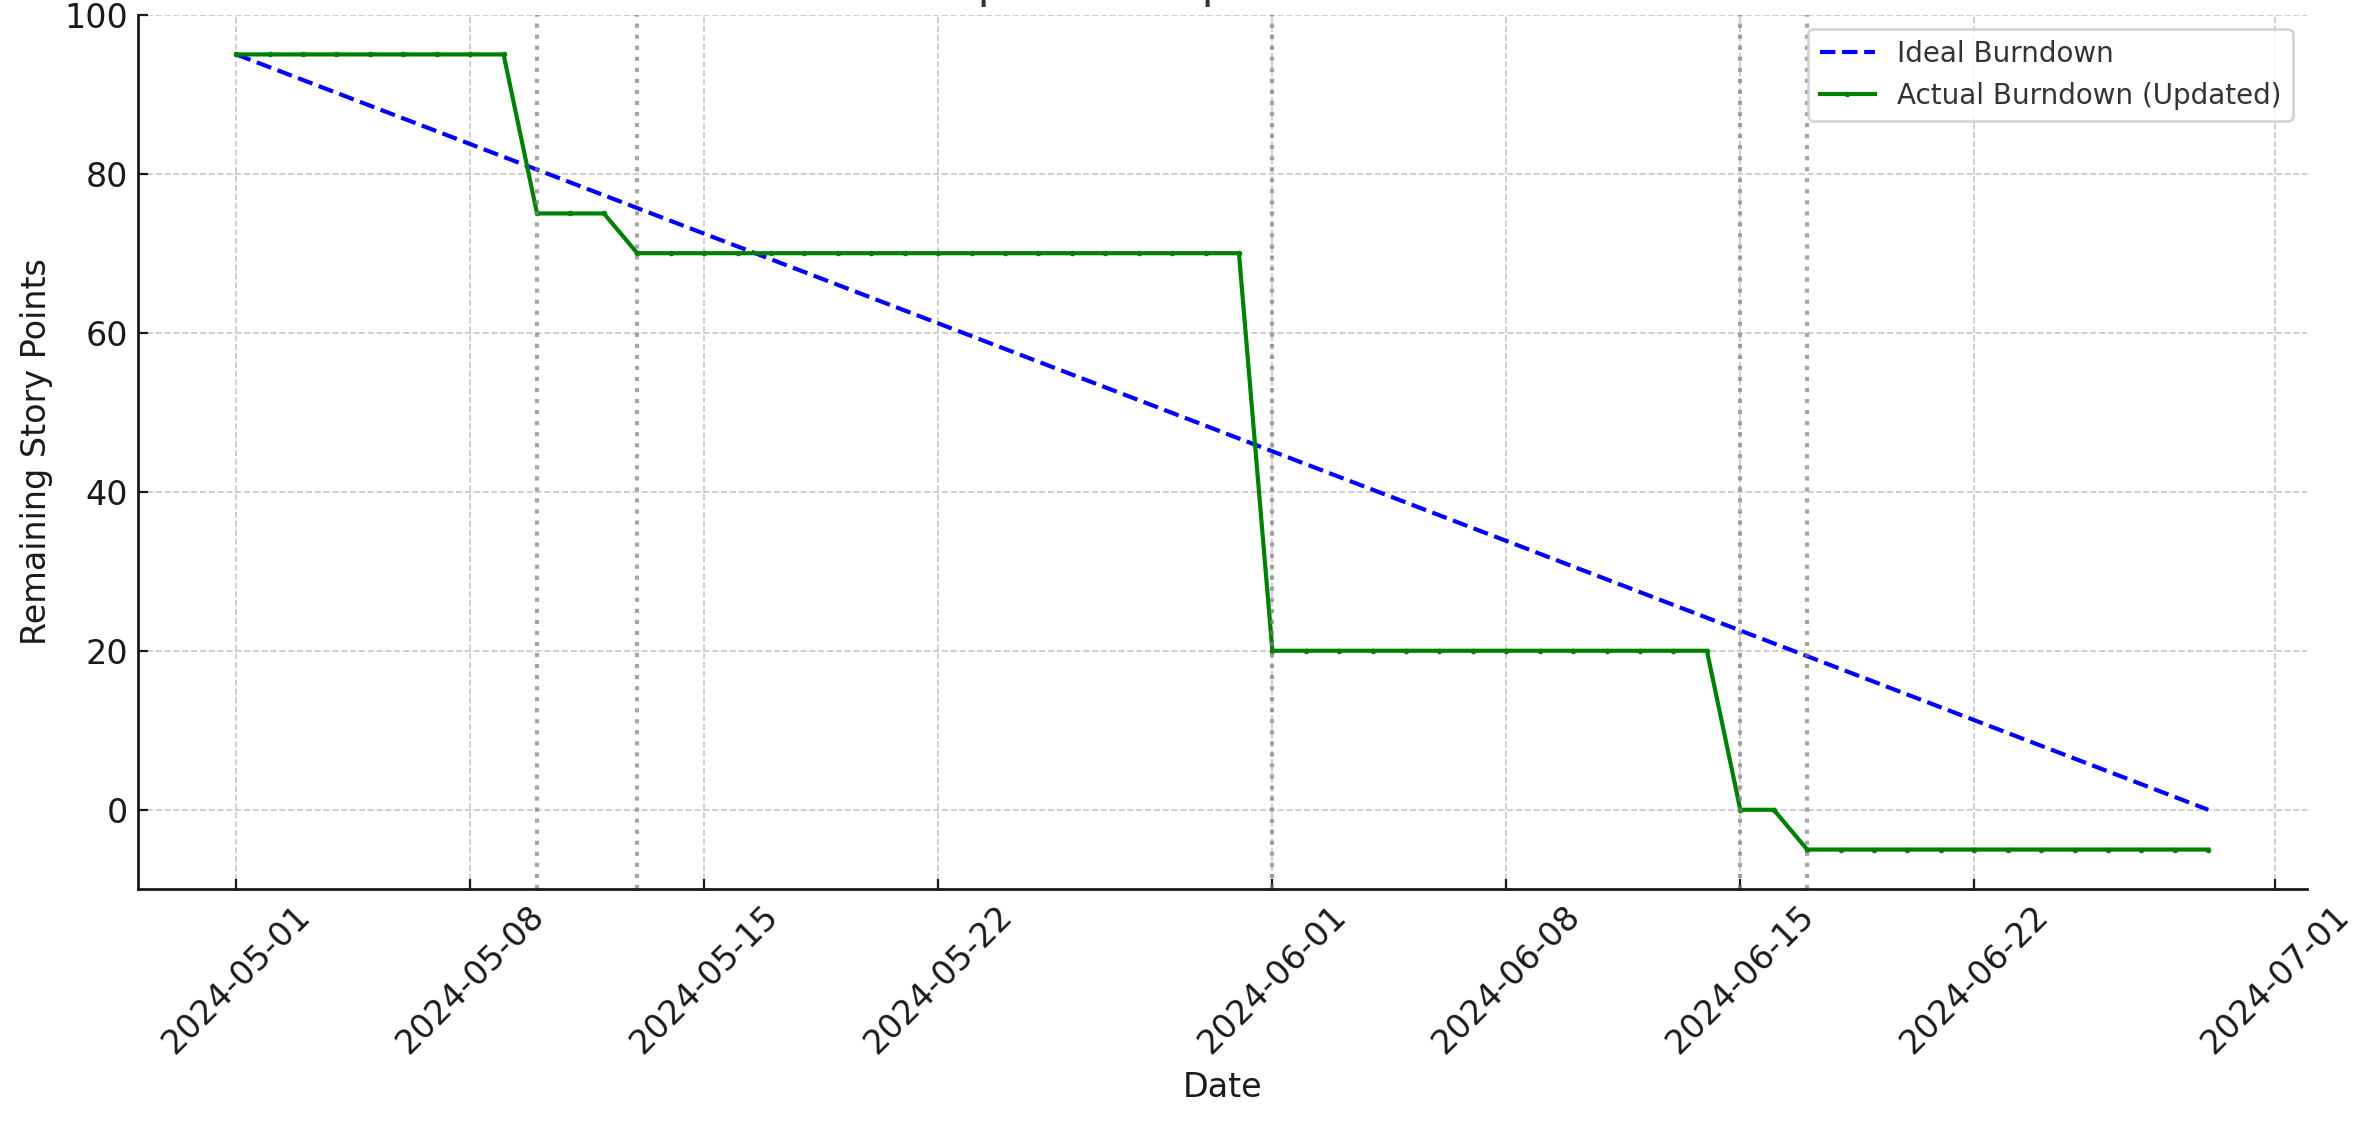
\includegraphics[width=0.8\textwidth]{./figs/burndown.png}
    \caption{Burn Down Chart for Sprint 1 (Prototype)}\label{fig:burndown}
\end{figure}

\section{Technology Stack}
This section describes the technologies used in the development of the LexiFlow system.  The following technologies were identified for their capacity to meet the project's requirements:

\begin{enumerate}[label= (\alph*)]
    \item \textbf{Vue.js:} A JavaScript framework for creating user interfaces.  Vue.js was chosen for its reactive and compiler-optimized rendering system. It will be used to create the frontend of the web application.
    \item \textbf{Node.js:} a JavaScript runtime based on Chrome's V8 engine. It was chosen for its non-blocking and event-driven architecture. That makes it suitable for developing scalable network applications. It will be used for server-side logic and user request management. Furthermore, It will act as the control center of our backend services, handling requests from the frontend and coordinating with the database and python microservices.
    \item \textbf{MongoDB:} A NoSQL database that stores data in flexible JSON-style documents.  MongoDB was selected due to its intuitive document model, which pairs unique objects with distinct documents, thereby simplifying data management. This makes it ideal for storing user-generated material, audio/video metadata, and processed subtitles.
    \item \textbf{FastApi:} A modern, high-performance web framework that aims to simplify the development of APIs with Python, using standard Python type hints. FastAPI was chosen because of its ease of use and automatic documentation creation. It will be used by the backend services to convert the python scripts into RESTful APIs, allowing our Node.js server to communicate with the services that handle audio processing, transcription, and translation.
    \item \textbf{SileroVAD:} Silero VAD works effectively with audios from a variety of domains with a range of background noise and quality levels. It was trained on a massive dataset that included over 6000 languages. It was chosen for its high accuracy and ease of use. It will be used to detect speech segments and segment them into sentence-level chunks.
    \item \textbf{Whisper:} a powerful automated speech recognition system that was trained on a diverse dataset of multilingual speech data. It was chosen for its high accuracy and ability to handle various languages and accents. It will be used to transcribe the audio content into text, providing the foundation for further processing.
    \item \textbf{SeamlessM4Tv2:} Meta's multilingual and multimodal machine translation model, will be utilized to translate Mandarin text into English.  it was chosen for its high-quality translation capabilities across multiple languages, including Mandarin and English.
    \item \textbf{PyPinyin:} A Python library for converting Chinese characters to pinyin.  PyPinyin will be used to provide pronunciation assistance for Mandarin text, making learning easier for users.
\end{enumerate}

The LexiFlow development process uses automated workflows to ensure smooth updates. As shown in Figure~\ref{fig:ci_cd}, developers first commit code changes to Git for version control. GitHub Actions then automatically builds and tests the code. Finally, Docker packages the working application for deployment through Nginx. This automated pipeline helps catch errors early and ensures stable releases.

The figure clearly shows how these steps connect with our planning and monitoring activities, keeping development efficient and reliable. This approach supports our hybrid Agile methodology by enabling frequent updates while maintaining system stability.

\begin{figure}[H]
    \centering
    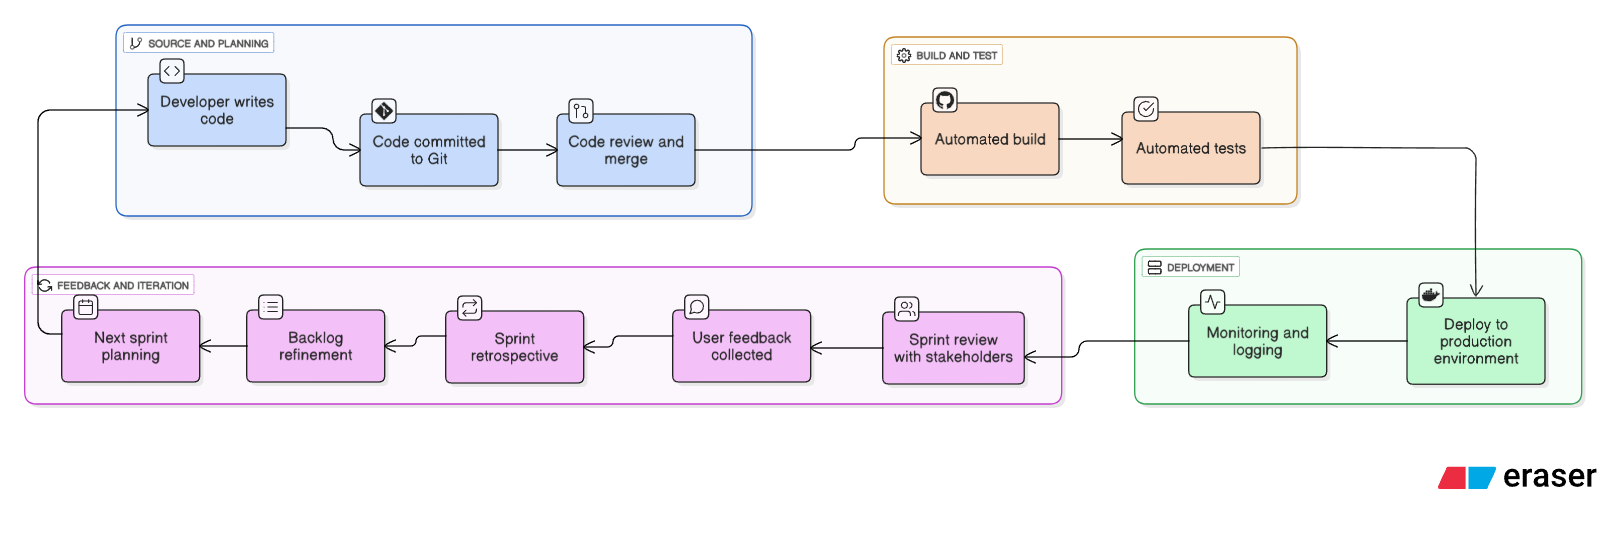
\includegraphics[width=1\textwidth]{./figs/ci_cd.png}
    \caption{CI/CD Pipeline for LexiFlow}\label{fig:ci_cd}
\end{figure}

\section{System Requirement Analysis}
This section provides information about system requirements that includes all hardware, software and other requirements. These details will be useful for meeting the functional and performance criteria and thus guarantee a successful development and operation process of the system described above.

\subsection{Hardware Requirements}
For the LexiFlow system, the following hardware requirements are necessary to ensure optimal deployment and user experience:
\begin{enumerate}[label= (\alph*)]
    \item \textbf{Server:} A dedicated server with at least 16 GB of RAM, 8 CPU cores, and 500 GB of SSD storage to handle the backend processing, database management, and API requests. Also a GPU with at least 8 GB of VRAM is must for efficient processing of audio content, especially for tasks like automatic speech recognition and machine translation.
    \item \textbf{Development Machines:} To run development environments, testing frameworks, and local databases, development machines should have a minimum of 8 GB of RAM, enough storage (at least 256 GB SSD), and a modern multi-core processor.
    \item \textbf{Client Devices:} Users should have access to devices with at least 4 GB of RAM and a modern web browser (Chrome, Firefox, Safari) to interact with the LexiFlow web application.
\end{enumerate}

\subsection{Software Requirements}
The LexiFlow system will require the following software components:
\begin{enumerate}[label= (\alph*)]
    \item \textbf{Operating System:} An operating system that is Linux-based (e.g., Ubuntu 22.04 or later) for the server environment to ensure stability and performance.
    \item \textbf{Web Server:} Nginx as the web server to handle HTTP requests and serve the LexiFlow web application.
    \item \textbf{Database:} MongoDB for storing user data, audio/video metadata, and processed subtitles.
    \item \textbf{Version Control:} Git to manage code changes and manage versions.
    \item \textbf{Network Protocols:} SSH to securely access the server remotly.
    \item \textbf{IDE:} Visual Studio Code, providing features like code completion, debugging, and version control integration.
    \item \textbf{Visual Design Tools:} Enterprise Architect to design the system architecture and UML diagrams. Figma to create user interface mockups.
\end{enumerate}



\section{Chapter Summary}
This chapter guides through the approach that was taken by LexiFlow with special emphasis on the hybrid Agile framework that combines both iterative development with structured phases. That way, the project could be agile enough to adapt to changing needs but still possess milestone checks. The technology stack has also been discussed in detail with the rationale of each decision. Lastly, the hardware and software requirements are also outlined, which sets the stage of a successful implementation in the subsequent phases.

\chapter{REQUIREMENT ANALYSIS AND DESIGN}
\section{Introduction}
This chapter provides an overview of the phases of requirement analysis and design stages for the LexiFlow project, which shows the way for the development of a systematically organised language learning system designed for the UTM community. The chapter adheres to a systematic way of identification and analysis of specific requirements of various stakeholders through structured interactions like surveys and interviews.

After the detailed requirement analysis is conducted, the chapter then proceeds to design the system. This involves looking at the design of a system architecture supporting seamless interactions between the various components of LexiFlow. This involves designing the modular structure of the system and how those different modules communicate with each other, ensuring that the architecture affects the set-out goals of the project.

\section{Requirements Gathering and Analysis}

The requirements for the LexiFlow project were analysed meticulously through an interview session with the stakeholders from UTM Language Academy. This was an essential process in detailing the limitations of the existing system and what specific needs the stakeholders have for the proposed LexiFlow platform. Their information indicated the dire necessity for an automated solution that effectively processes authentic Mandarin content, providing learners with synchronized audio, pinyin, and English translations.

A greater emphasis was placed during the analysis on the following key functionalities identified as necessary for improving the overall effectiveness of the system: features for user evaluation, such as flashcards, quizzes and others as well as themed playlist features to ensure learning is more organized and structured. These kinds of features are expected to improve the learning process.  Figure~\ref{fig:use_case} below details the use case diagram of LexiFlow implementing the features stated previously.

\begin{figure}[h!]
    \centering
    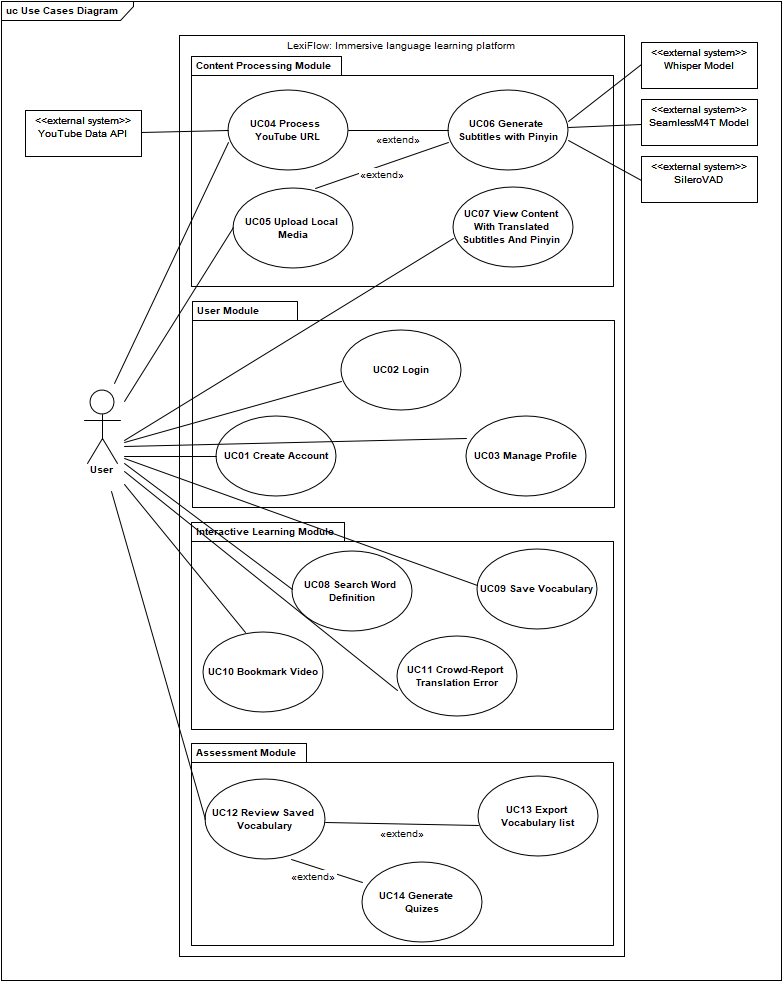
\includegraphics[width=0.8\textwidth]{./figs/use_cases.png}
    \caption{Use Case Diagram of LexiFlow}\label{fig:use_case}
\end{figure}

The requirement analysis phase ended with a proper understanding of the system specifications and functionalities. Such requirements are aimed at guiding the subsequent phases in the design and development of a system. Although the project development is done purposely to align with the needs and expectations of the UTM community, LexiFlow also looks toward overcoming the deficiencies of the current system and innovative features enhancing user experience and safety. Such an approach is likely to result in the development of a final product well tailored to
satisfy specific demands of the UTM community.

\subsection{Functional Requirements}
The functional requirements of LexiFlow are derived from the use case diagram (Figure~\ref{fig:use_case}) and are shown in Table~\ref{tab:functional_requirements}.
\begin{longtable}{>{\centering\arraybackslash}m{1.2cm} >{\centering\arraybackslash}m{3cm} >{\arraybackslash}m{8cm}}
    \caption{Functional Requirements of LexiFlow System}\label{tab:functional_requirements}                                     \\
    \toprule
    \textbf{ID} & \textbf{Name}                  & \textbf{Description}                                                         \\
    \midrule
    \endfirsthead
    \multicolumn{3}{l}{\textit{(Continued from previous page)}}                                                                 \\
    \toprule
    \textbf{ID} & \textbf{Name}                  & \textbf{Description}                                                         \\
    \midrule
    \endhead
    \midrule
    \multicolumn{3}{r}{\textit{(Continued on next page)}}                                                                       \\
    \endfoot
    \bottomrule
    \endlastfoot
    UC01        & Create Account                 & Allows new users to register and create an account in the system.            \\
    UC02        & Login                          & Enables registered users to authenticate and access the system.              \\
    UC03        & Manage Profile                 & Allows users to view and update their personal information and preferences.  \\
    UC04        & Process YouTube URL            & Handles the processing of YouTube video URLs for content extraction.         \\
    UC05        & Upload Local Media             & Enables users to upload media files from their local device for processing.  \\
    UC06        & Generate Subtitles             & Automatically creates subtitles for processed video content.                 \\
    UC07        & Find Translated Content        & Provides functionality to locate translated versions of content.             \\
    UC08        & Search Word Definition         & Allows users to search for definitions of words within the learning module.  \\
    UC09        & Save Vocabulary                & Enables users to save new vocabulary words for later review.                 \\
    UC10        & Bookmark Video                 & Allows users to bookmark specific video segments for future reference.       \\
    UC11        & Crowd-Report Translation Error & Provides a mechanism for users to collaboratively report translation errors. \\
    UC12        & Review Saved Vocabulary        & Enables users to review and practice vocabulary they have previously saved.  \\
    UC13        & Export Vocabulary list         & Allows users to export their vocabulary lists for use outside the system.    \\
    UC14        & Generate Quizes                & Automatically creates quizes from saved vocabulary for study purposes.       \\
\end{longtable}

As an example, the use case for processing YouTube URLs (UC04), shown in Table~\ref{tab:use_case_uc04}, involves key actors such as the user and the YouTube Data API. The system extracts video content by validating the URL, retrieving metadata, and checking the duration of the video.

All use cases, including detailed descriptions of the normal flow, alternative flows (such as handling invalid duration or restricted content), and exception flows, are fully documented in the Software Requirements Specification (SRS). The complete use case specifications can be found in Appendix~\ref{app:srs}.

\begin{longtable}{|>{\columncolor[HTML]{D9D9D9}}l|p{10cm}|}
    \caption{Use Case Description for UC04 \textless{}Process YouTube URL\textgreater{}}\label{tab:use_case_uc04}
    {}                                                                                                                                                                                                        \\
    \hline
    \textbf{Use Case ID}           & UC04                                                                                                                                                                     \\
    \hline
    \textbf{Use Case Name}         & Process YouTube URL                                                                                                                                                      \\
    \hline
    \textbf{Description}           & This use case allows an authenticated user to submit a YouTube video URL for automated transcription, translation, and synchronized subtitle generation within LexiFlow. \\
    \hline
    \textbf{Actor(s)}              & User, YouTube Data API                                                                                                                                                   \\
    \hline
    \textbf{Pre-conditions}        &
    1. The user is successfully logged into their LexiFlow account.                                                                                                                                           \\
                                   & 2. The LexiFlow system has internet access to reach YouTube.                                                                                                             \\
                                   & 3. System has active connection to YouTube Data API                                                                                                                      \\
    \hline
    \textbf{Normal Flow (NF)}      &
    1. User navigates to "Upload/Process Content" section                                                                                                                                                     \\
                                   & 2. User selects option to process YouTube URL                                                                                                                            \\
                                   & 3. User inputs valid YouTube video URL                                                                                                                                   \\
                                   & 4. User submits URL for processing                                                                                                                                       \\
                                   & 5. System validates URL and fetches video stream                                                                                                                         \\
                                   & 6. System initiates content processing pipeline                                                                                                                          \\
                                   & 7. System notifies user that processing has started                                                                                                                      \\
    \hline
    \textbf{Alternative Flow (AF)} &
    AF1: Invalid YouTube URL                                                                                                                                                                                  \\
                                   & \quad 1. If URL is invalid or video not found:                                                                                                                           \\
                                   & \quad \quad 1.1 System displays "Invalid YouTube URL" error                                                                                                              \\
                                   & \quad \quad 1.2 Prompts user to enter correct URL                                                                                                                        \\
                                   & AF2: Restricted/Private Video                                                                                                                                            \\
                                   & \quad 1. If video is regionally restricted or private:                                                                                                                   \\
                                   & \quad \quad 1.1 System displays access restriction error                                                                                                                 \\
                                   & \quad \quad 1.2 Use case terminates unsuccessfully                                                                                                                       \\
    \hline
    \textbf{Exception Flow (EF)}   &
    EF1: Processing Pipeline Failure                                                                                                                                                                          \\
                                   & \quad 1. If content processing encounters critical error:                                                                                                                \\
                                   & \quad \quad 1.1 System logs detailed error                                                                                                                               \\
                                   & \quad \quad 1.2 Displays generic failure message                                                                                                                         \\
                                   & \quad \quad 1.3 Use case terminates unsuccessfully                                                                                                                       \\
                                   & EF2: Network Error During Fetch                                                                                                                                          \\
                                   & \quad 1. If network issue prevents video fetching:                                                                                                                       \\
                                   & \quad \quad 1.1 System displays network error message                                                                                                                    \\
                                   & \quad \quad 1.2 Prompts user to check connection                                                                                                                         \\
                                   & \quad \quad 1.3 Use case terminates unsuccessfully                                                                                                                       \\
    \hline
    \textbf{Post-conditions}       &
    1. YouTube video content is successfully extracted                                                                                                                                                        \\
                                   & 2. Content processing pipeline is initiated                                                                                                                              \\
                                   & 3. User receives processing status notification                                                                                                                          \\
    \hline
    \textbf{Special Requirements}  &
    1. System has internet access to reach YouTube                                                                                                                                                            \\
                                   & 2. YouTube video processing capabilities                                                                                                                                 \\
    \hline
\end{longtable}

\subsection{Non-Functional Requirements}
Non-functional requirements define the quality attributes, system performance, and constraints that LexiFlow must adhere to. These requirements are crucial for ensuring the system's reliability, usability, and maintainability. The non-functional requirements are summarized in Table~\ref{tab:non_functional_requirements}.

\begin{longtable}{>{\centering\arraybackslash}m{1.2cm} >{\centering\arraybackslash}m{3cm} >{\arraybackslash}m{8cm}}
    \caption{Non-Functional Requirements}
    \label{tab:non_functional_requirements}                                                                                                                         \\
    \hline
    \textbf{ID} & \textbf{Type}   & \textbf{Description}                                                                                                            \\
    \hline
    \endfirsthead
    \multicolumn{3}{l}{\textit{(Continued from previous page)}}                                                                                                     \\
    \hline
    \textbf{ID} & \textbf{Type}   & \textbf{Description}                                                                                                            \\
    \hline
    \endhead
    \hline
    \multicolumn{3}{r}{\textit{(Continued on next page)}}                                                                                                           \\
    \endfoot
    \hline
    \endlastfoot
    NFR-001     & Performance     & The system shall process and validate YouTube URLs within 3 seconds to ensure responsive user experience.                       \\
    \hline

    NFR-002     & Localization     & The system shall support display text in at least two languages: English and Mandarin.                                                     \\
    \hline

    NFR-003     & Backup & System data shall be backed up automatically every 24 hours and stored securely \\
\end{longtable}

\section{Architectural Design}

The Pipe and Filter architectural pattern organizes processing into a series of discrete components, called filters, connected by pipes. Each filter performs a specific transformation or processing step on the data and passes the result to the next filter through a pipe. This modular approach enhances scalability, maintainability, and reusability, as filters can be developed, tested, and replaced independently. The clear separation of concerns also simplifies debugging and future system extensions.

The Pipe and Filter pattern is particularly well-suited for LexiFlow's audio processing pipeline, where each filter can handle a specific task such as voice activity detection, speech recognition, translation, and pinyin generation. This modularity allows for easy integration of new processing steps or replacement of existing ones without affecting the overall system architecture.


As shown in Figure~\ref{fig:pipe_and_filter}, the LexiFlow system architecture consists of several key components:


\begin{enumerate}[label= (\alph*)]
    \item \textbf{User Interface (UI):} The front-end application built with Vue.js, providing an interactive platform for users to upload media, view subtitles, and manage vocabulary. Considered as the source of data in the Pipe and Filter architecture.
    \item \textbf{Backend Services:} Implemented using Node.js and FastAPI, these services handle user requests, process audio and video content, and are considered as pipes in the Pipe and Filter architecture.
    \item \textbf{Audio Processing Pipeline:} A series of filters that perform tasks such as voice activity detection (SileroVAD), automatic speech recognition (Whisper), translation (SeamlessM4Tv2), and pinyin generation.
    \item \textbf{Database:} MongoDB is used to store user profiles, processed content metadata, subtitles, and vocabulary lists. Considered as the sink of data in the Pipe and Filter architecture.
\end{enumerate}

\begin{figure}[H]
    \centering
    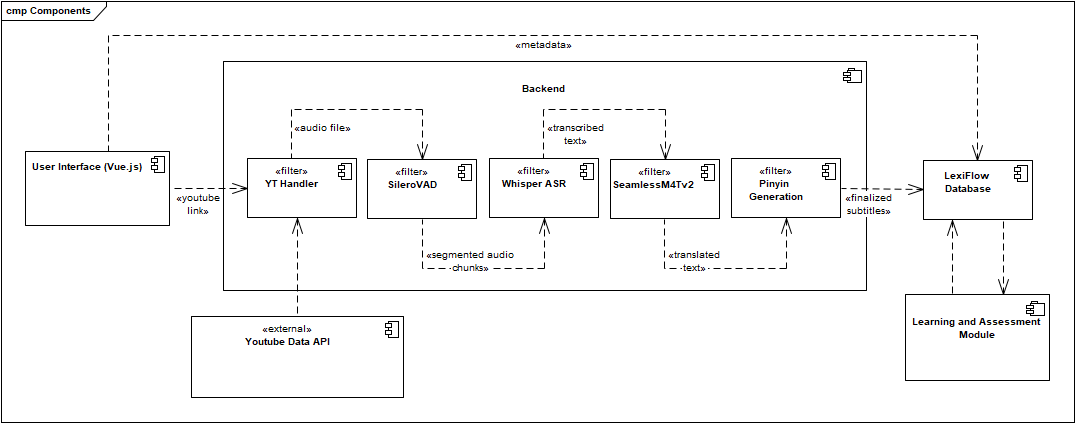
\includegraphics[width=0.95\textwidth]{./figs/arch.png}
    \caption{LexiFlow System Architecture}\label{fig:pipe_and_filter}
    \smallskip
    \begin{flushleft}
        \small * The figure illustrates the Pipe and Filter architecture of LexiFlow, showing the modular processing components and their interactions.
    \end{flushleft}
\end{figure}

\section{Chapter Summary}
Chapter 4 of the thesis delves into the requirement analysis and system design for LexiFlow, outlining a comprehensive approach to developing a language learning platform. The chapter begins with a systematic exploration of stakeholders' needs through interactive sessions, setting the foundation for detailed documentation in the Software Requirements Specification (SRS, Appendix~\ref{app:srs}) and Software Design Document (SDD, Appendix~\ref{app:sdd}). It further details the pipe-and-filter architectural approach, ensuring scalability and efficiency, and discusses the user interface design, which is integral for enhancing user interaction and system functionality. This methodical approach not only aligns with the project's objectives but also ensures a robust framework for the successful implementation and operation of LexiFlow. The system was subsequently validated through automated end-to-end testing and User Acceptance Testing, documented in Chapter 5 and Appendices~\ref{app:test-execution-report} and~\ref{app:uat-report}, rather than a separate, standalone Software Test Document.


\chapter{System Implementation}\label{chap:implementation}

\section{Introduction}
This chapter discusses the technical implementation of LexiFlow. It first revisits the Pipe and Filter architecture from Chapter 4 and shows how it materialised in code, then walks through the core learning features --- subtitle generation, flashcards, quizzes, crowd-sourced error reporting, and a companion browser extension --- followed by a brief account of the DevOps and deployment setup and the verification work carried out on the finished system.

The frontend is implemented in \textbf{React 18 with TypeScript} (built with Vite) rather than the Vue 3 framework originally proposed in Chapter 4, because the required library ecosystem --- the Auth0 React SDK, TanStack Query, and the interactive subtitle-viewer components --- was more mature on React at implementation time. The backend retains the dual-service design from the design phase: a Node.js (Express) server for business logic and orchestration, and a Python FastAPI server for the AI media pipeline. Supporting capabilities outside these four features (account management, profile, and onboarding UX) are not elaborated on here, as they follow standard, unremarkable implementations.

\section{Architecture in Practice: Pipe and Filter}
Chapter 4 proposed a Pipe and Filter architectural style for the media-processing subsystem: each stage of subtitle generation is an independent filter that consumes the previous stage's output and passes its own output downstream, with no stage aware of any other beyond its immediate neighbour. Figure~\ref{fig:media_pipeline} shows how this was realised: a source video is downloaded and normalised by FFmpeg, transcribed by a cloud Whisper API, translated by an LLM, and finally annotated with pinyin and HSK levels before being persisted as a subtitle document.

\begin{figure}[H]
    \centering
    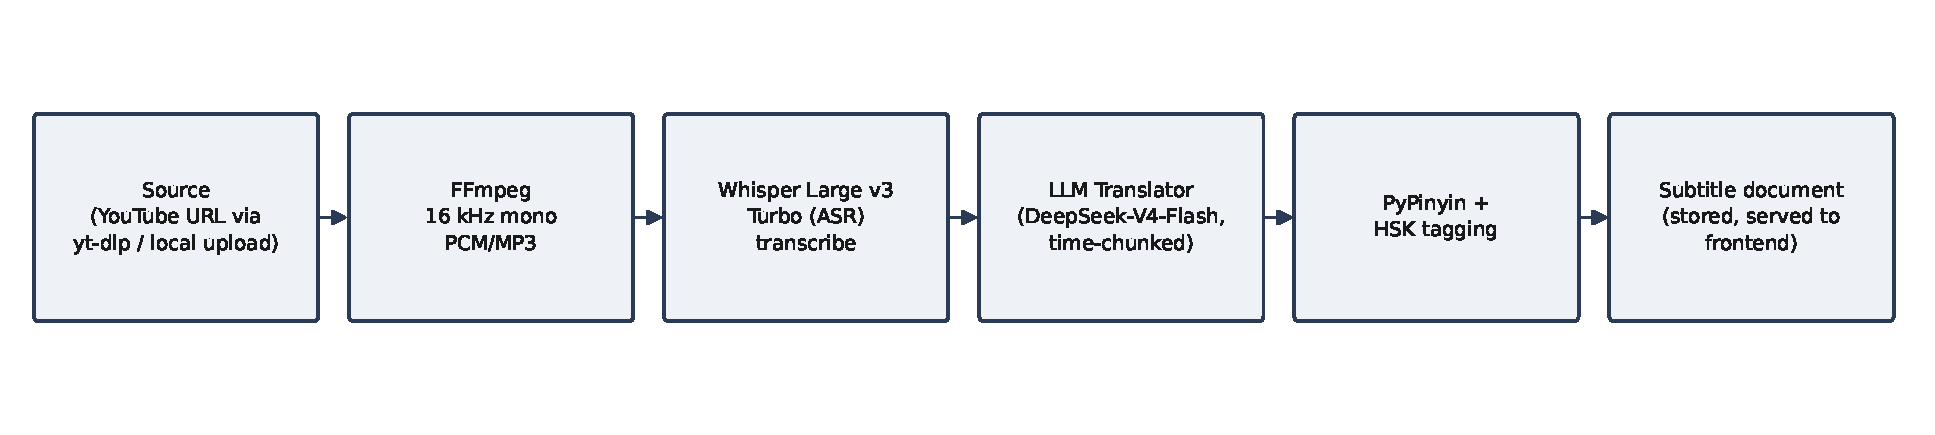
\includegraphics[width=0.95\textwidth]{./figs/fig_media_pipeline.pdf}
    \caption{Pipe and Filter realisation of the media-processing pipeline}\label{fig:media_pipeline}
\end{figure}

Figure~\ref{lst:pipeline} shows the orchestrator that wires these filters together. Each step reports its own progress and elapsed time independently, and a failure in one step does not require any of the other filters to know why --- it simply does not receive input.

\begin{figure}[H]
\begin{verbatim}
async def run_pipeline(job_id, url, is_local=False):
    # 1. Download (yt-dlp) or accept local upload
    file_path = await asyncio.to_thread(download_video, url, job_id)

    # 2. Transcribe (Whisper Large v3 Turbo, FFmpeg-normalised audio)
    transcription = await asyncio.to_thread(api_transcribe, file_path)

    # 3. Translate (LLM, time-chunked) + pinyin/HSK annotation
    translation = await asyncio.to_thread(api_translate, transcription)

    # 4. Post-process into the final subtitle document shape
    end_result = await asyncio.to_thread(api_postprocess, translation)
\end{verbatim}
\caption{Simplified pipeline orchestrator (\texttt{backend-fastapi/api.py})}\label{lst:pipeline}
\end{figure}

Each filter is independently substitutable: the transcription filter, for instance, was switched from a locally-hosted Whisper model to a cloud Whisper API partway through development without any change to the filters before or after it, since the contract between stages (a list of timestamped text segments) never changed.

\section{Core Feature: Generate Subtitles (UC06)}
Subtitle generation is the entry point to every other feature in LexiFlow. A submitted video is transcribed by the \textbf{Whisper Large v3 Turbo} automatic speech recognition model, translated sentence-by-sentence into English by a chat-completion language model, and annotated with tone-marked pinyin via \textbf{PyPinyin} and per-character HSK difficulty levels. Figure~\ref{lst:translate} shows the translation filter: segments are batched into five-minute time windows (giving the model cross-sentence context without risking a truncated response) and the model is constrained to return one JSON translation per input sentence, in order.

\begin{figure}[H]
\begin{verbatim}
SYSTEM_PROMPT = (
    "...Respond with a JSON object of the exact form "
    '{{"translations": ["...", ...]}} containing exactly '
    "{count} strings, in the same order as the input...")

for chunk in _chunk_by_time(segments, chunk_seconds=300):
    translations = _request_translations(chunk_texts, ...)
    for segment, translated_text in zip(chunk, translations):
        segment["translated_text"] = translated_text
\end{verbatim}
\caption{Simplified LLM translation filter (\texttt{backend-fastapi/src/llm/translator.py})}\label{lst:translate}
\end{figure}

The resulting subtitle is rendered on the watch page as a bilingual, pinyin-annotated transcript synchronised to the video. Every Chinese token is individually tappable: tapping a character or word opens an instant CC-CEDICT dictionary lookup (Figure~\ref{fig:ss_subtitles}) without interrupting playback, directly fulfilling Search Word Definition (UC08) and feeding Save Vocabulary (UC09).

\begin{figure}[H]
    \centering
    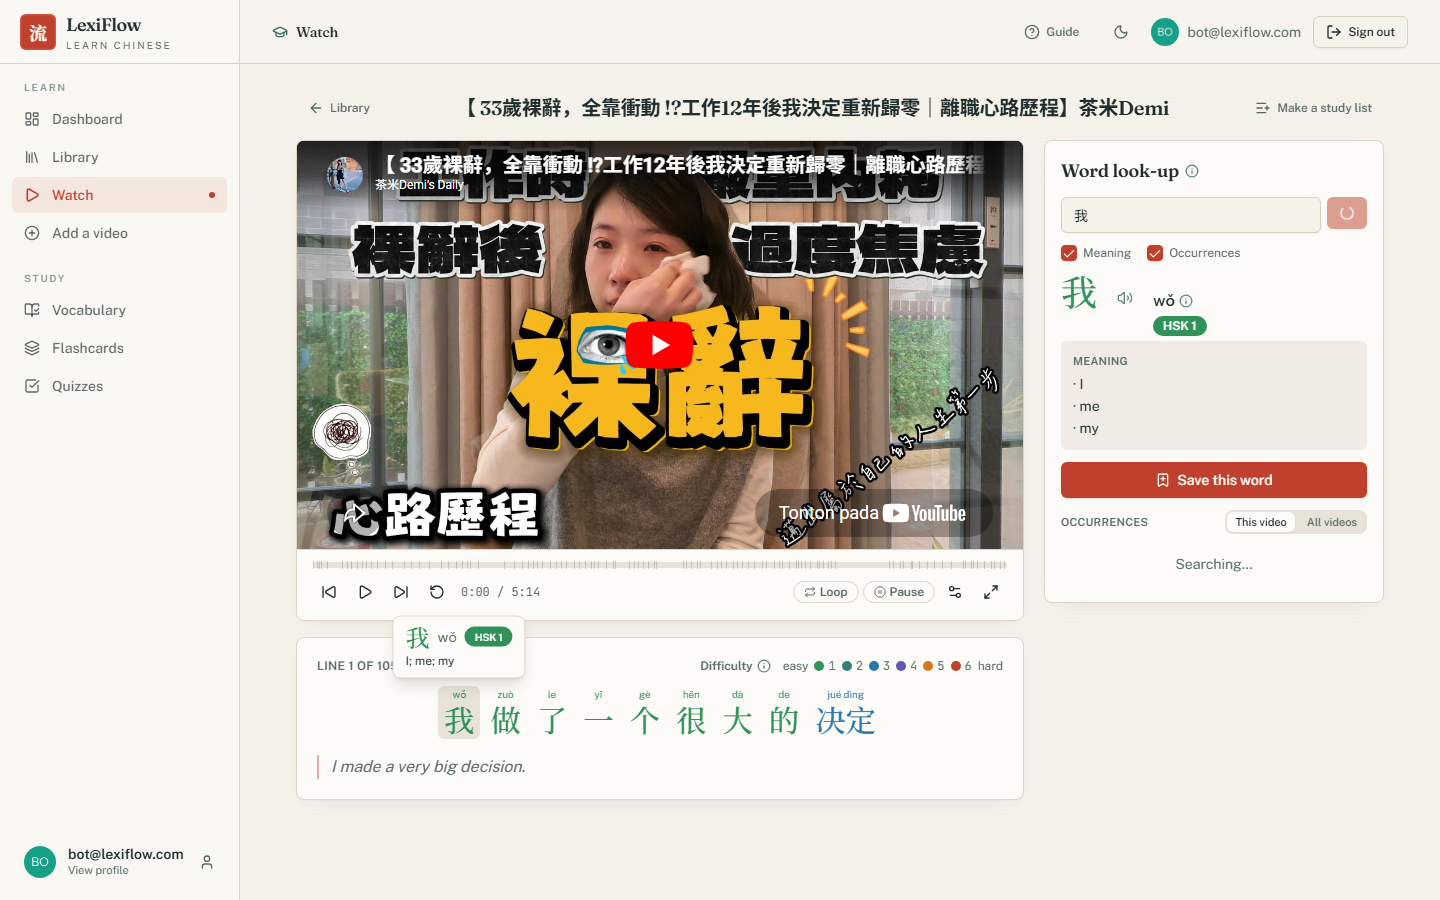
\includegraphics[width=0.7\textwidth]{./figs/fig_ss_subtitles.png}
    \caption{Bilingual subtitle playback with tap-to-look-up dictionary panel}\label{fig:ss_subtitles}
\end{figure}

\section{Core Feature: Generate and Review Flashcards (UC13)}
Saved vocabulary is reinforced through a spaced-repetition flashcard system implementing the \textbf{FSRS (Free Spaced Repetition Scheduler) algorithm}, the same model used by the modern Anki ecosystem. Figure~\ref{fig:fsrs_growth} shows how the scheduled interval for a single item grows across consecutive successful reviews: early reviews are a day or two apart, while well-retained items are pushed weeks into the future, concentrating review effort where it is needed.

\begin{figure}[H]
    \centering
    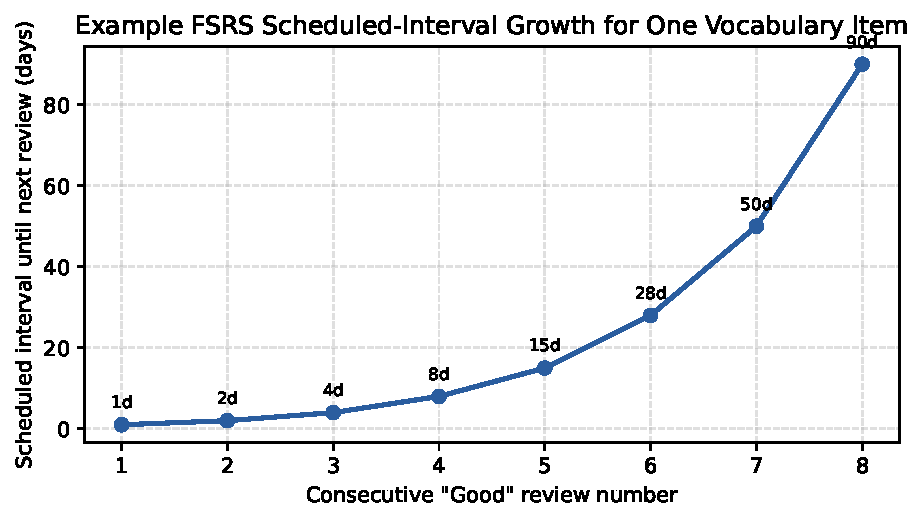
\includegraphics[width=0.7\textwidth]{./figs/fig_fsrs_growth.pdf}
    \caption{Example FSRS scheduled-interval growth for one vocabulary item}\label{fig:fsrs_growth}
\end{figure}

Figure~\ref{lst:fsrs} shows the core scheduling function. Each grade (Again/Hard/Good/Easy) recomputes the item's Stability and Difficulty and derives the next review date directly from the published FSRS weight parameters, implemented in-house rather than via a third-party scheduling service.

\begin{figure}[H]
\begin{verbatim}
function calculateFsrs(card, rating) {
    let { stability, difficulty, state } = card;
    if (card.state === 0 || stability === 0) {
        difficulty = clamp(FSRS_W[4] - FSRS_W[5] * (rating - 3), 1, 10);
        stability  = rating === 1
            ? FSRS_W[0]
            : FSRS_W[1] + FSRS_W[2] * (rating - 2)
                + FSRS_W[3] * Math.pow(rating - 1, 0.5);
    } else {
        const r = Math.pow(1 + 0.1 * (card.elapsedDays / stability), -1);
        difficulty = clamp(difficulty - FSRS_W[6] * (rating - 3), 1, 10);
        stability = /* FSRS stability-growth formula, rating-dependent */ ...;
    }
    const scheduledDays = clamp(Math.round(stability), 1, 365);
    return { stability, difficulty, scheduledDays, nextReviewDate: ... };
}
\end{verbatim}
\caption{Simplified FSRS scheduler (\texttt{backend-node/.../flashcards.service.js})}\label{lst:fsrs}
\end{figure}

The frontend presents this as a flip-style card: the front shows only the Chinese word, and flipping reveals pinyin and meaning alongside the four grading buttons, each labelled with its resulting interval (Figure~\ref{fig:ss_flashcards}) so the learner can see the consequence of their self-assessment immediately.

\begin{figure}[H]
    \centering
    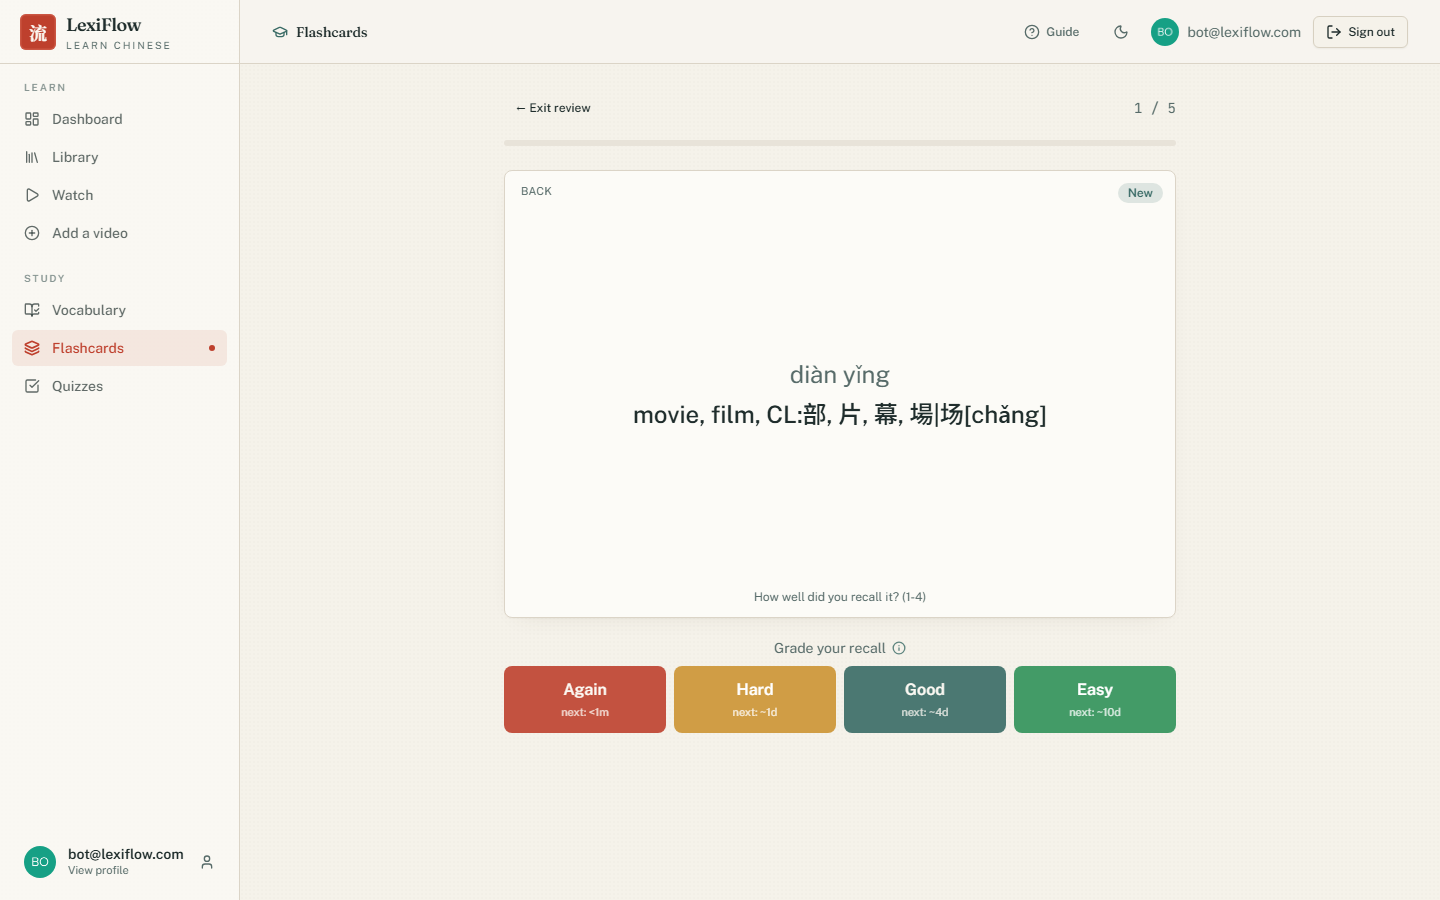
\includegraphics[width=0.7\textwidth]{./figs/fig_ss_flashcards.png}
    \caption{Flashcard review: back face with recall grading buttons}\label{fig:ss_flashcards}
\end{figure}

\section{Core Feature: Generate Quizzes (UC14)}
LexiFlow can synthesise a quiz on demand from any vocabulary list, mixing four question formats: multiple choice, fill-in-the-blank, true/false, and short answer (Figure~\ref{fig:ss_quizzes}). Fill-in-the-blank questions are produced by masking the target word inside a saved example sentence; multiple-choice and true/false questions additionally require plausible wrong answers (distractors).

\begin{figure}[H]
    \centering
    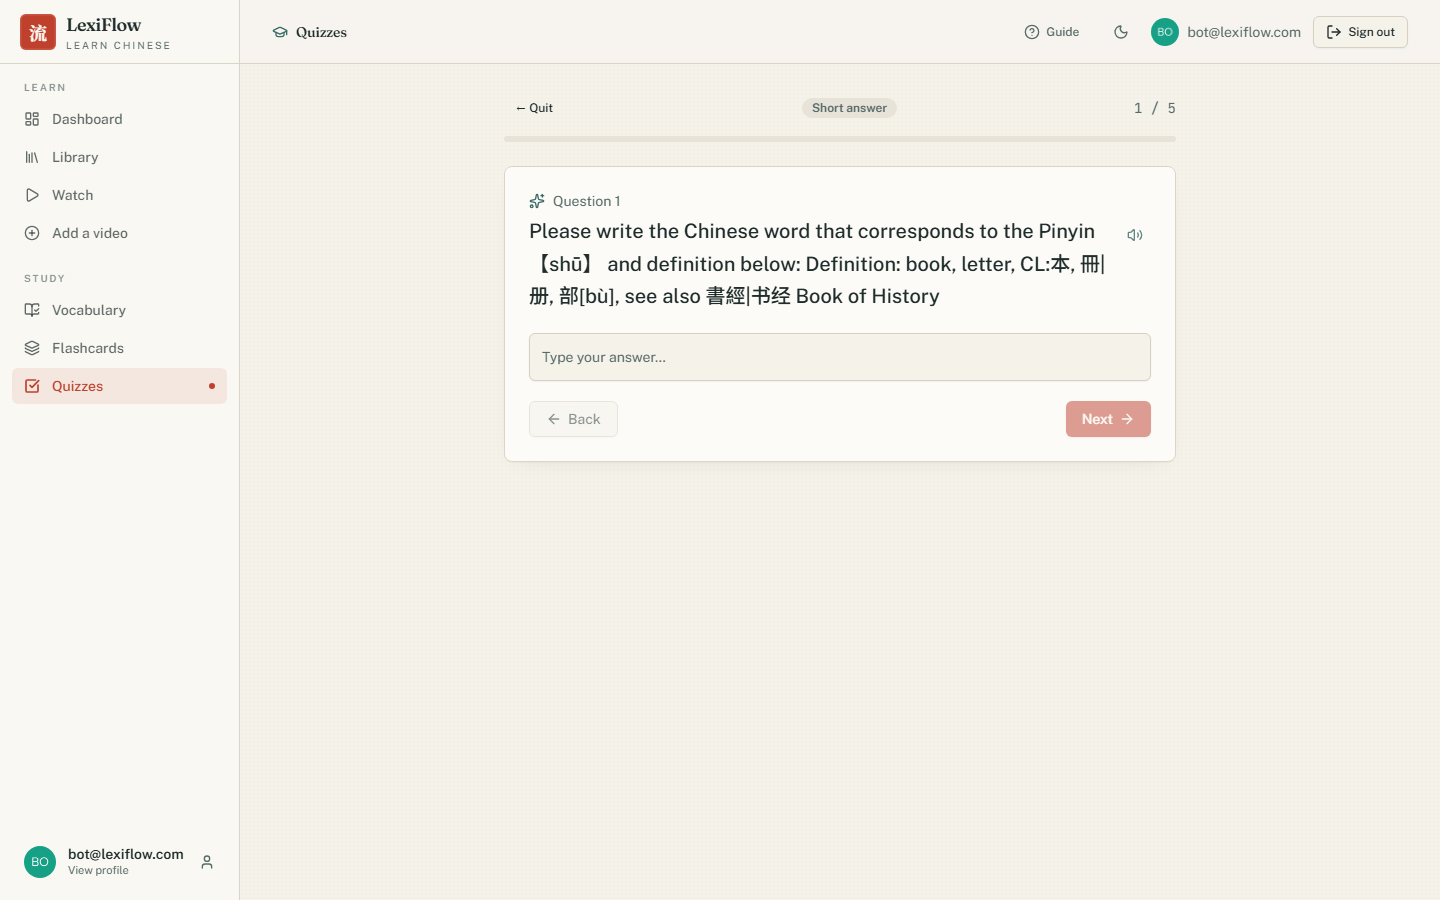
\includegraphics[width=0.7\textwidth]{./figs/fig_ss_quizzes.png}
    \caption{A generated short-answer quiz question}\label{fig:ss_quizzes}
\end{figure}

Short-answer responses cannot be checked by exact string matching, since a correct answer may be phrased many ways. Figure~\ref{lst:judge} shows the grading filter: an exact match short-circuits immediately, otherwise the reference answer and the learner's response are sent to an LLM, which is required to return a structured verdict.

\begin{figure}[H]
\begin{verbatim}
def evaluate_short_answer(self, correct_reference, user_response):
    if ref_clean == resp_clean:
        return {"score": 1.0, "feedback": "Exact", "is_correct": True}

    content = self.provider.chat_complete(
        system=SYSTEM_PROMPT, user=json.dumps({...}), json_mode=True)
    result = json.loads(content)
    return {"score": result["score"], "feedback": result["feedback"],
            "is_correct": result["is_correct"]}
\end{verbatim}
\caption{Simplified short-answer judge (\texttt{backend-fastapi/services/quiz/judge.py})}\label{lst:judge}
\end{figure}

Distractor selection for multiple-choice questions combines this same LLM-based contextual-plausibility judgement with two lightweight local heuristics: a pinyin Levenshtein-distance similarity (to catch words that sound alike) and a radical/Unicode similarity score (to catch words that look alike). The three scores are summed and the highest-ranked candidates from the same HSK tier are chosen, so a generated distractor is plausible without ever being an accidental synonym of the correct answer.

\section{Core Feature: Crowd-Reporting of Translation Errors (UC11)}
Any viewer can flag a subtitle line as wrong, choosing a category --- translation, pinyin, transcription, or other (Figure~\ref{fig:ss_crowdreport}). A line is only escalated for correction once it passes a deliberately conservative double threshold (Figure~\ref{lst:flag}): at least three distinct reporters, \emph{and} at least 25\% of everyone who viewed that line, so a single dissatisfied viewer cannot flag content unilaterally.

\begin{figure}[H]
    \centering
    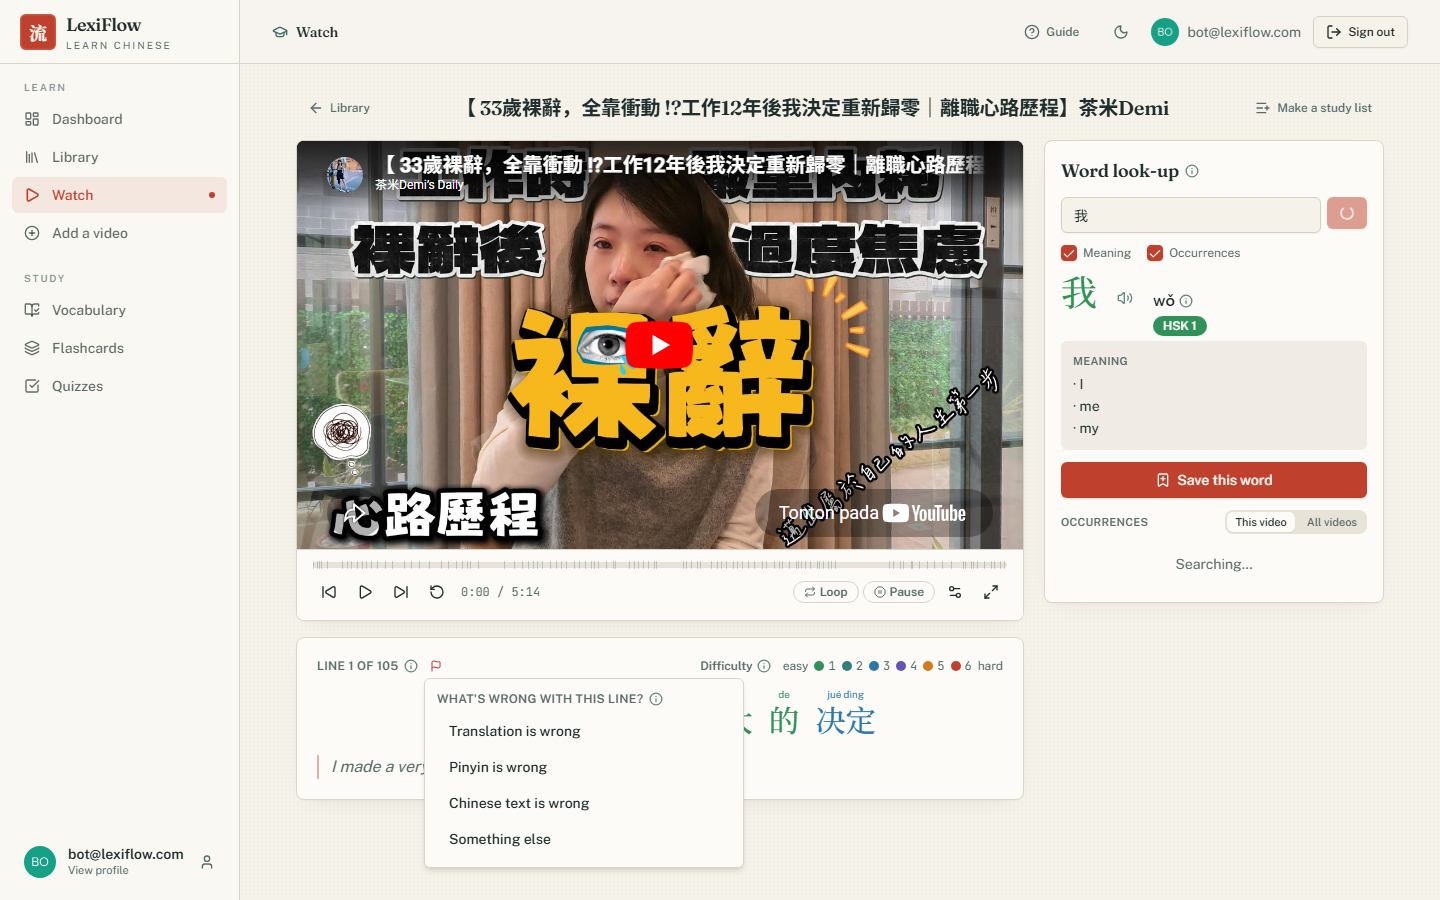
\includegraphics[width=0.7\textwidth]{./figs/fig_ss_crowdreport.png}
    \caption{Reporting a subtitle line and choosing an error category}\label{fig:ss_crowdreport}
\end{figure}

\begin{figure}[H]
\begin{verbatim}
const FLAG_MIN_REPORTS = 3;
const FLAG_THRESHOLD_PERCENT = 0.25;
...
flagged: c.count >= FLAG_MIN_REPORTS
      && (c.count / viewerCount) >= FLAG_THRESHOLD_PERCENT
\end{verbatim}
\caption{Simplified flag threshold (\texttt{backend-node/.../reports.service.js})}\label{lst:flag}
\end{figure}

Once flagged, the line is corrected immediately rather than queued for a human moderator: the reported segment, three segments of surrounding context, and an instruction specific to the error category are sent to \textbf{Meta's Llama 3.3 70B} model, constrained to JSON-mode output. The original timestamps are always re-applied server-side rather than trusted to the model, so a hallucinated value can never desynchronise the subtitle from the audio, and the correction is stored as a separate, reversible patch rather than overwriting the original transcription.

\section{Core Feature: Browser Extension}
To bring LexiFlow's bilingual subtitle experience to content the user is already watching, a companion browser extension overlays graded Chinese subtitles, word lookup, and text-to-speech directly on top of the YouTube player, removing the need to copy a video URL into the main platform first.

\begin{figure}[H]
    \centering
    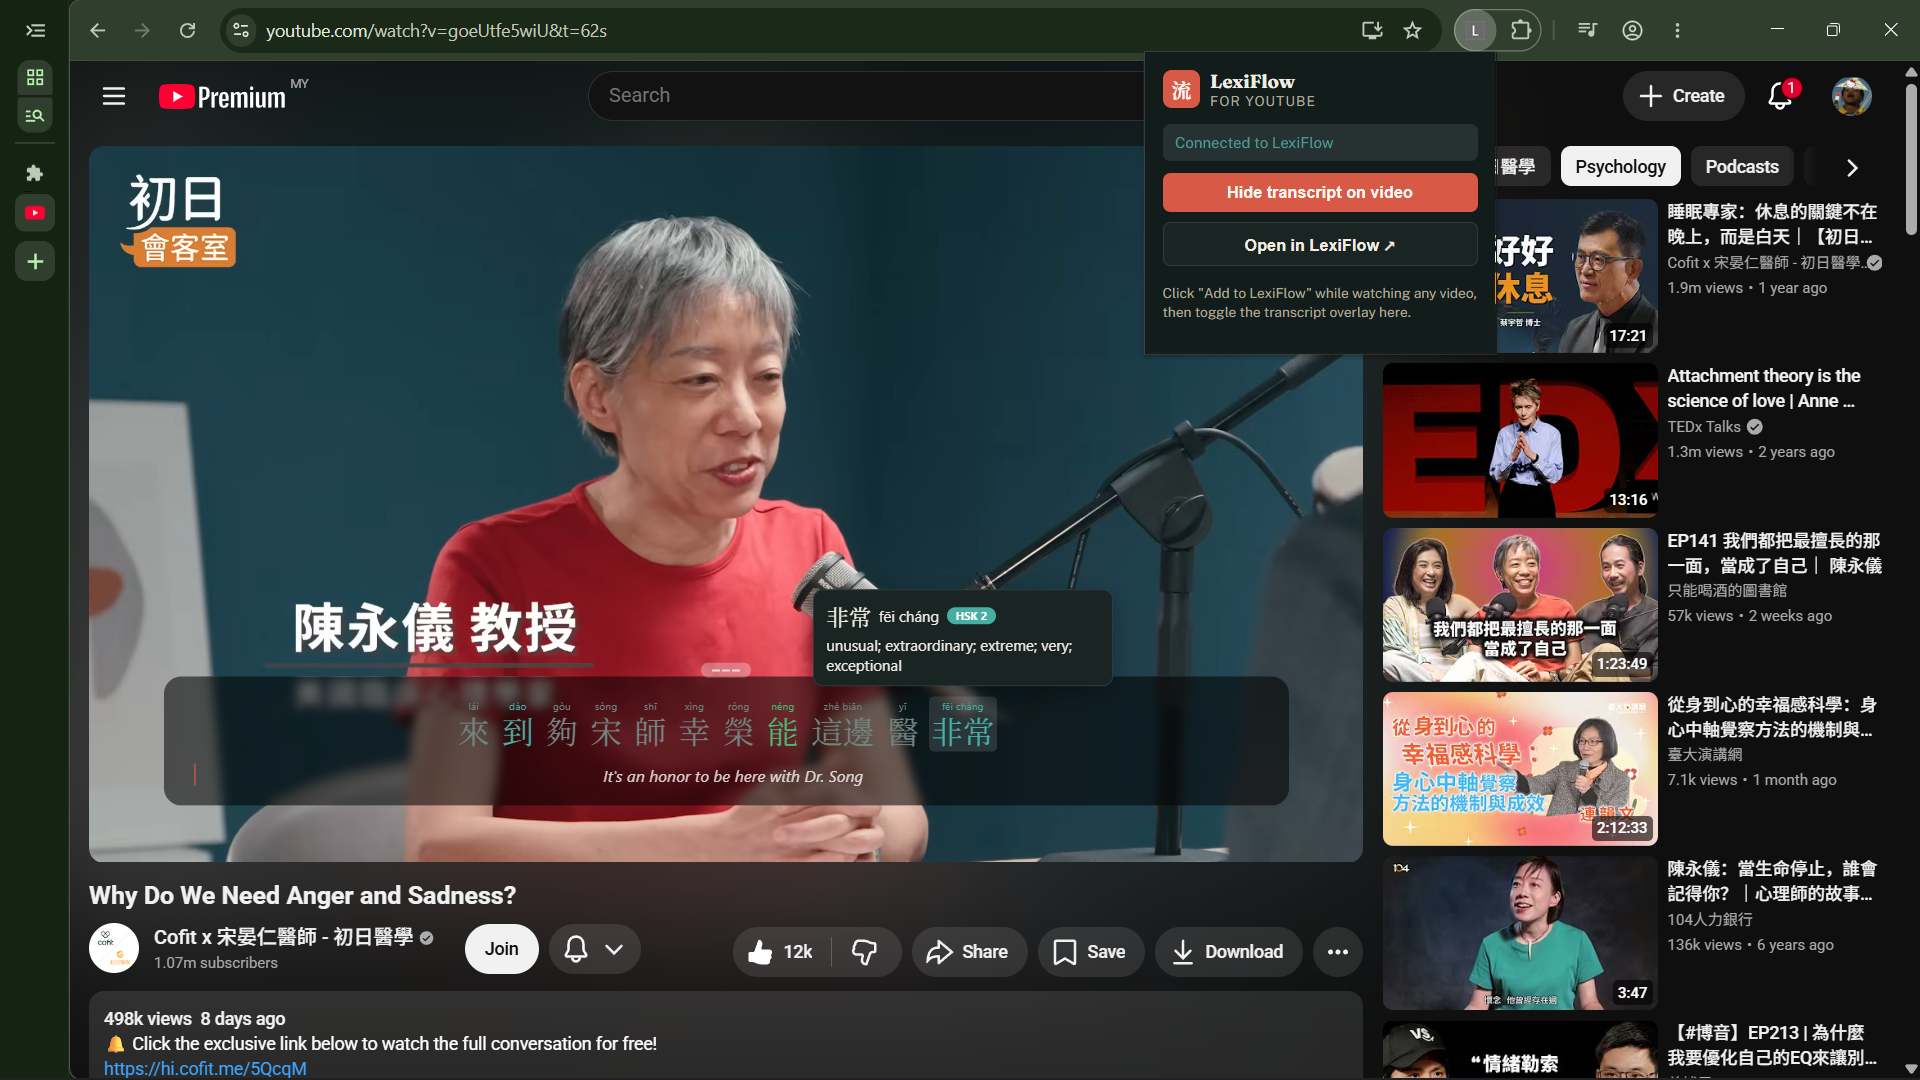
\includegraphics[width=0.95\textwidth]{./figs/fig_browser_extension.png}
    \caption{LexiFlow browser extension overlay on YouTube}\label{fig:ss_extension}
\end{figure}

\section{DevOps and Deployment}
Figure~\ref{fig:deployment_topology} summarises where each part of the system runs. The frontend is a static build served from \textbf{Vercel}'s edge CDN. The Node.js backend, the FastAPI worker, and PostgreSQL all run together on a single \textbf{Tencent Cloud Lighthouse} VM via Docker Compose, with a \textbf{SaladPool} instance retained as a rarely-used failover worker. \textbf{GitHub Actions} builds and pushes a container image to GHCR on every push to \texttt{main} and redeploys the VM automatically, so no manual deployment step is required. All AI inference --- transcription, translation, quiz grading, and segment correction --- is delegated to externally hosted language models (Whisper Large v3 Turbo, DeepSeek-V4-Flash, and Llama 3.3 70B), so the deployment itself requires no GPU.

\begin{figure}[H]
    \centering
    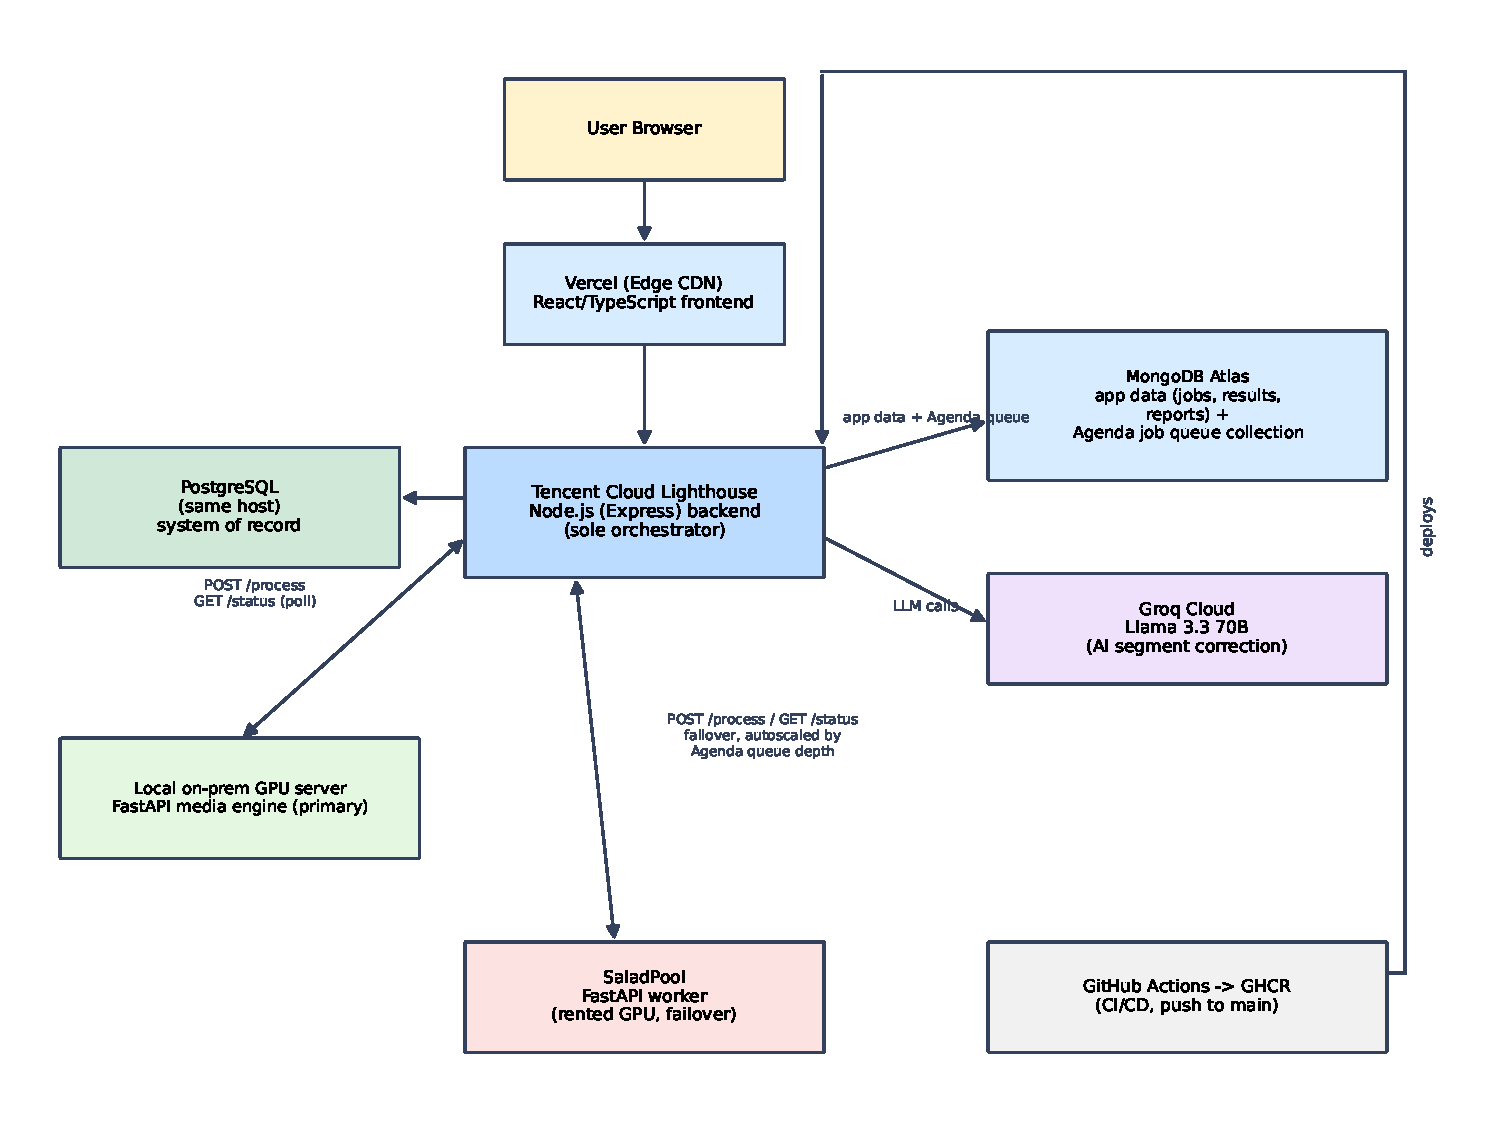
\includegraphics[width=0.95\textwidth]{./figs/fig_deployment_topology.pdf}
    \caption{LexiFlow deployment topology}\label{fig:deployment_topology}
\end{figure}

\section{Verification and Validation}
The system was verified at two complementary levels. First, an automated end-to-end Playwright suite was run directly against the live test deployment, covering UC01 through UC14. This produced 25 passes, 4 failures, and 1 documented skip out of 30 test cases; the 4 failures traced to two genuine, reproducible defects (an undismissable onboarding tour and a missing single-page-application fallback route) rather than to flaws in the test scripts. The full methodology, per-test-case results, and root-cause analysis are presented in Appendix~\ref{app:test-execution-report}.

Second, User Acceptance Testing was carried out with four participants spanning the user groups identified in Chapter 4: a previously-struggling Mandarin learner, a self-directed learner with a domain-specific vocabulary need, a native-speaker reviewer assessing transcription/translation accuracy, and the instructor stakeholder. Feedback confirmed the value of the tap-to-look-up, vocabulary-saving, and quiz-generation workflow, while surfacing two honest findings for future work: an accuracy gap against commercial-grade captioning, and the absence of classroom-management features, neither of which was scoped as a functional requirement in Chapter 4. Full participant profiles, scenarios, and acceptance-criteria analysis are presented in Appendix~\ref{app:uat-report}.

\section{Chapter Summary}
This chapter showed how the Pipe and Filter architecture from Chapter 4 was implemented as an independently-substitutable pipeline, then detailed the implementation of the four core learning features --- subtitle generation, flashcards, quizzes, and crowd-sourced correction --- each combining a deterministic local algorithm (FSRS, threshold checks, pinyin/visual similarity) with an LLM where open-ended judgement is genuinely required. The deployment was kept deliberately lightweight by delegating all AI inference to external APIs, and the resulting system was verified through both automated end-to-end testing and User Acceptance Testing, with all defects found during verification traced to specific, reproducible root causes rather than to architectural flaws.

\chapter{CONCLUSION}
\section{Introduction}
This chapter will give an overview of the LexiFlow project's development, outcomes, and to what extent the project’s goals were achieved. It will emphasise the findings and insights, significant accomplishments and suggest areas for future improvement. This review outlines the overall effectiveness of the application for LexiFlow in addressing the concerns of educators, and learners, coupled with its future potential to improve and scale. The project of LexiFlow has been able to develop a good system of language learning, meeting the expectations set by users. Architecture and technology decisions taken in this project will be the solid base for any further enhancements. Through the relentless improvement and development, LexiFlow might stand out as one of the best language learning solutions for universities and across settings, being reliable and user-friendly to its users.

\section{Achievement of Project Objectives}
The LexiFlow project began with four main objectives, as elaborated in Section~\ref{sec:obj} of this paper. Each objective aimed at a better language learning experience through a user-friendly interface and robust audio processing pipeline. The following section discusses the level of performance for each of the project objectives, now that the system has been fully implemented, deployed to a live test environment, and evaluated through both automated testing and UAT:

\begin{enumerate}[label= (\alph*)]
    \item \textbf{Elicit Comprehensive Requirements from Stakeholders:} The first objective was to gather detailed requirements from stakeholders. This was successfully accomplished through a series of interviews with these stakeholders. The interactions with them provided valuable insights into the language learning needs and challenges within the UTM community. The requirements elicited formed the project’s functional and non-functional specifications. The Software Requirements Specification (SRS) included in Appendix~\ref{app:srs} documents these stated specifications. Therefore, this objective can be considered successfully achieved, with the system requirements effectively collected and analysed.
    \item \textbf{Design a Web-Based Platform:} The second objective focused on designing a web-based platform with an appropriate architectural design. The LexiFlow application was designed using a  Pipe and Filter architecture model. The use of Vue for the frontend development enabled the creation of an intuitive and responsive user interface, while both Python and Node.js provided robust backend services. The Software Design Document (SDD) attached in Appendix~\ref{app:sdd}, contains detailed design and documentation of the system. Thus, this objective can be considered successfully achieved.
    \item \textbf{Develop the Full Platform:} The third objective was to develop a language learning platform. Development of the system entails implementing the audio processing pipeline, which includes voice activity detection, automatic speech recognition, translation, and pinyin generation. The features were developed based on the elicited requirements and the design specifications.
    \item \textbf{Evaluate and Test the Functionality:} The final objective was to evaluate and test the functionality of the LexiFlow platform in improving the language learning experience. This was going to be done through extensive testing incorporating unit tests, integration tests, and user acceptance tests in the next phase which is PSM2. The Software Testing Documentation includes the preliminary test cases and test approaches, which are attached in the appendices (Appendix~\ref{app:std}). This objective will be considered complete once the project is fully developed and testing is conducted.
\end{enumerate}

\section{Service Enhancement and Practical Value}
Beyond meeting its stated objectives, LexiFlow delivers value along two of the three dimensions typically used to assess a system's practical worth: it enhances quality of service, and it increases quality of life for its users; it does not currently have demonstrated commercial value, since no pricing model, payment integration, or market validation has been attempted.

LexiFlow enhances quality of service by automating a task that the stakeholder interview (Appendix~\ref{app:stakeholder-interview-questions}) reported as taking 10-30 minutes of manual effort per simple three-minute video: transcribing, translating, and pinyin-annotating authentic Mandarin content. By reducing this to an automated pipeline that a learner or educator can trigger on demand, and by adding a crowd-correction mechanism so quality improves over time without re-doing that manual work, the system materially improves on the status quo described by the stakeholder, where authentic content was used sparingly because of this preparation cost.

LexiFlow increases quality of life for its users in ways independently confirmed during UAT (Appendix~\ref{app:uat-report}): a struggling learner reflected that the platform would likely have improved their actual exam outcome, and a professional working in a Mandarin-speaking environment described it as something they would use daily to reduce real workplace miscommunication, neither of which their prior study methods (classroom drills, generic apps, or textbooks) addressed. These are direct, user-reported improvements to learning outcomes and everyday communication confidence, rather than abstract or assumed benefits.

\section{Suggestions for Future Improvement}
Building on the findings from automated testing and UAT, the following improvements are recommended for future iterations of LexiFlow. First, the two confirmed defects identified during test execution, the undismissable onboarding tour (LF-BUG-01) and the missing SPA fallback route causing direct navigation to return a raw 404 (LF-BUG-02), should be fixed before any production rollout, as both directly block or degrade core navigation for first-time and returning users respectively. Second, the accuracy gap identified by the native-speaker UAT participant, between LexiFlow's self-hosted faster-whisper and LibreTranslate pipeline and YouTube's own commercial-grade auto-captioning, should continue to be narrowed; the crowd-reporting and AI-assisted correction feature already implemented (Chapter 5) is well-positioned to do this over time, and its effectiveness should be measured directly in a future evaluation round. Third, and most significantly, a classroom-management module, allowing an instructor to create a class, assign specific videos or quizzes as coursework, and view a lecturer-facing progress dashboard across their students, should be scoped and implemented; this was identified as the primary unmet need by the instructor stakeholder during UAT and was never part of the original functional requirements, making it the clearest candidate for the next phase of development. Beyond these evidence-based priorities, the usage of a more lightweight, Mandarin-only local model instead of a large multilingual model would reduce processing time and server VRAM usage, in turn lowering server operating costs, and switching to more efficient model runtimes such as ONNX or TensorRT would further reduce processing time and resource usage. Together, these changes would make LexiFlow more accurate, more complete for institutional use, and more efficient to operate.

\bibliographystyle{unsrtnat} % Use the "abbrvnat" BibTeX style for formatting the bibliography
\bibliography{reference} % Entries are in the refs.bib file

\appendix
\chapter{List of Prompts Used}
\pdfbookmark[0]{List of Prompts Used}{sec:list-of-prompts-used}
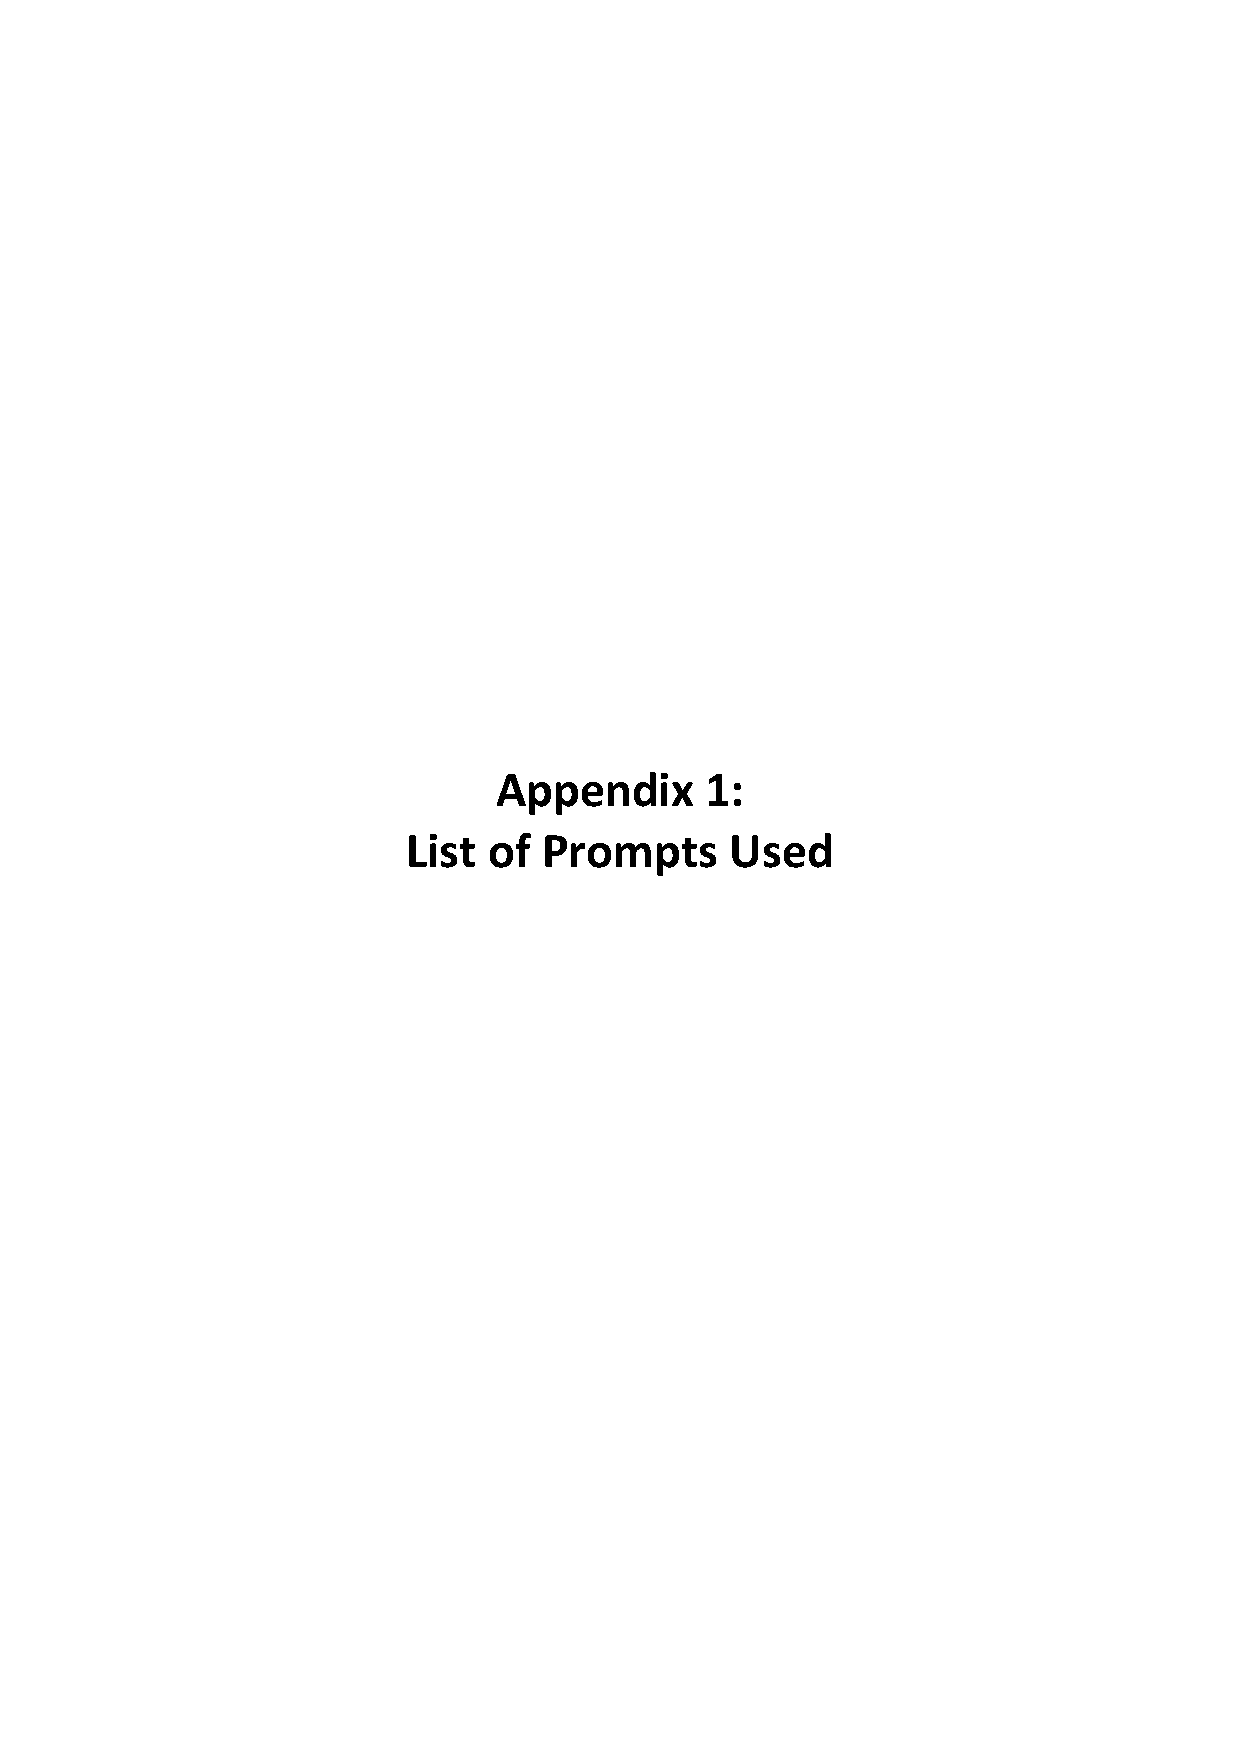
\includepdf[pages=-]{figs/prompts.pdf}

\chapter{Test Execution Report}\label{app:test-execution-report}
\pdfbookmark[0]{Test Execution Report}{sec:test-execution-report}
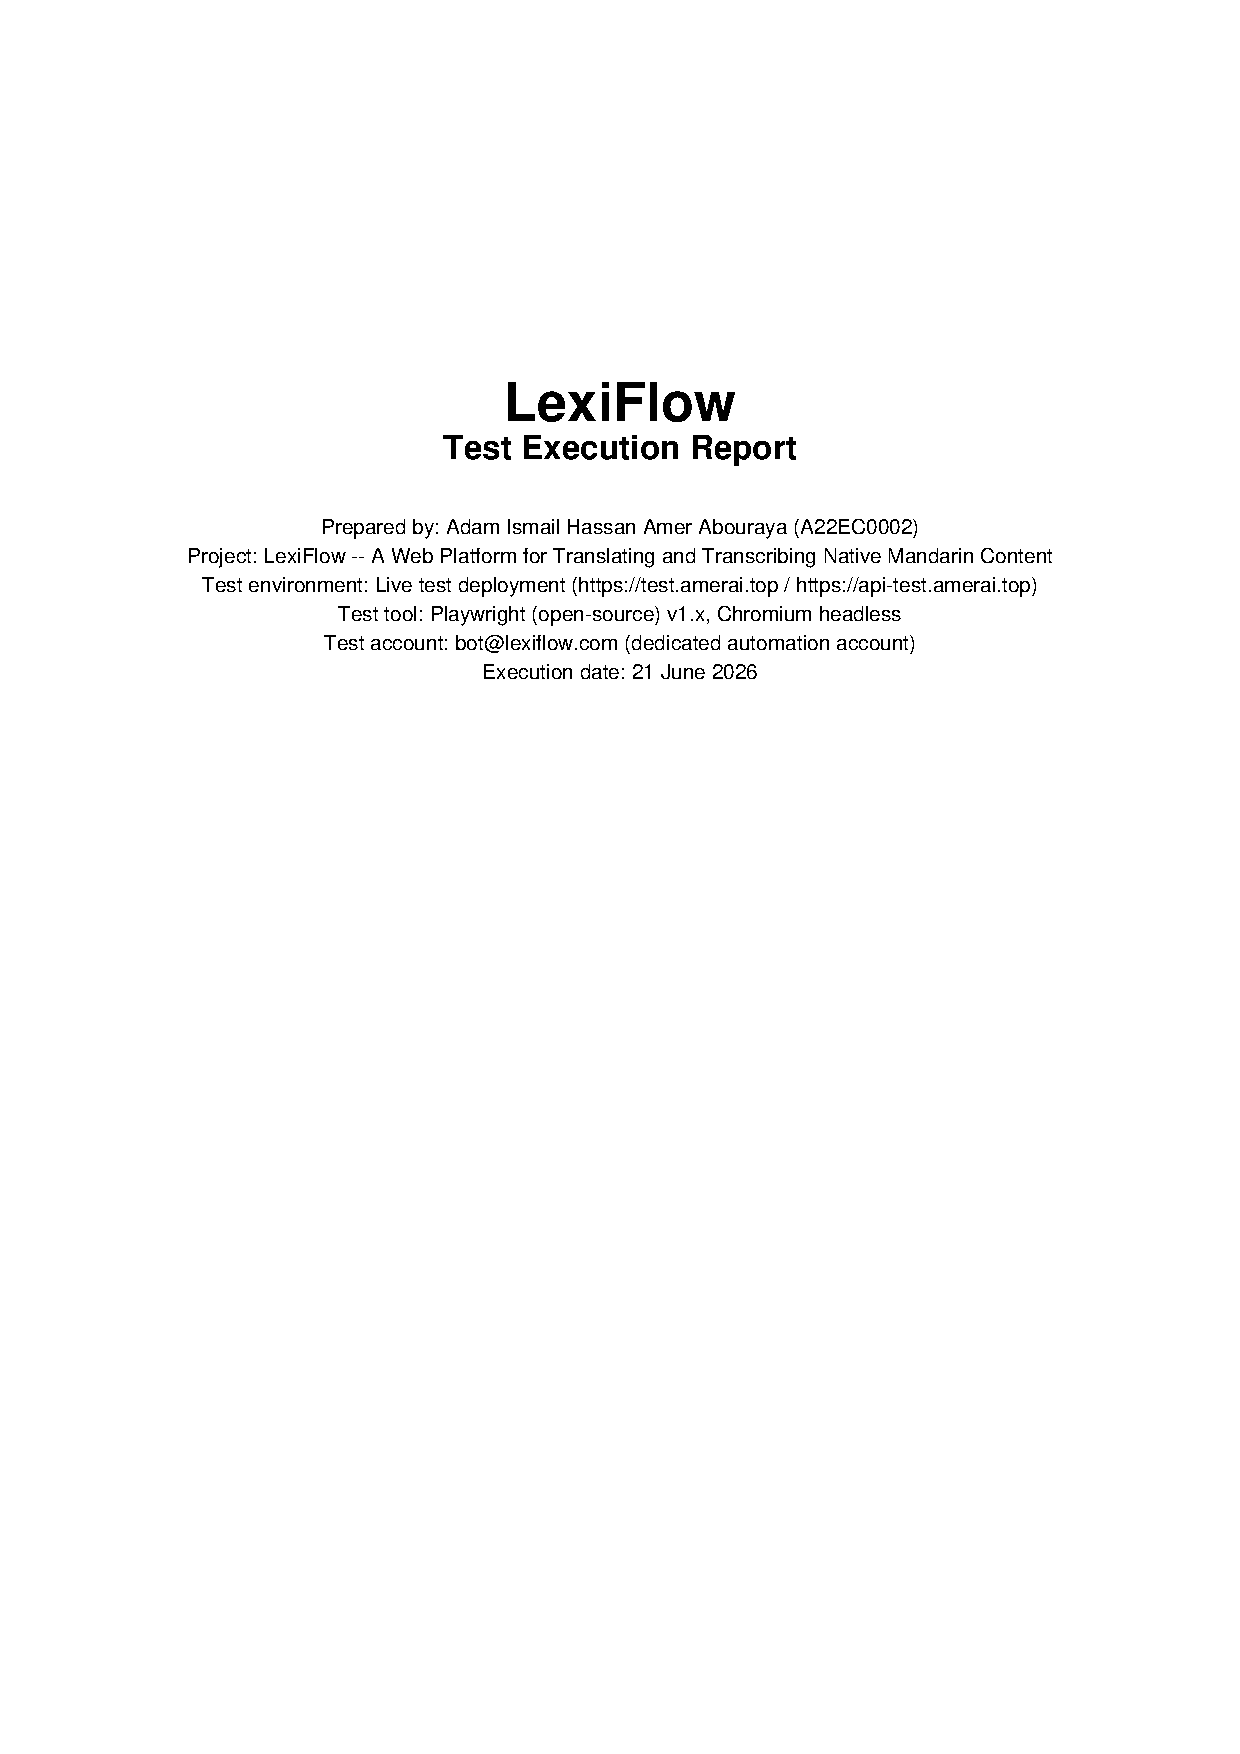
\includepdf[pages=-]{figs/test_execution_report.pdf}

\chapter{User Acceptance Test (UAT) Report}\label{app:uat-report}
\pdfbookmark[0]{User Acceptance Test (UAT) Report}{sec:uat-report}
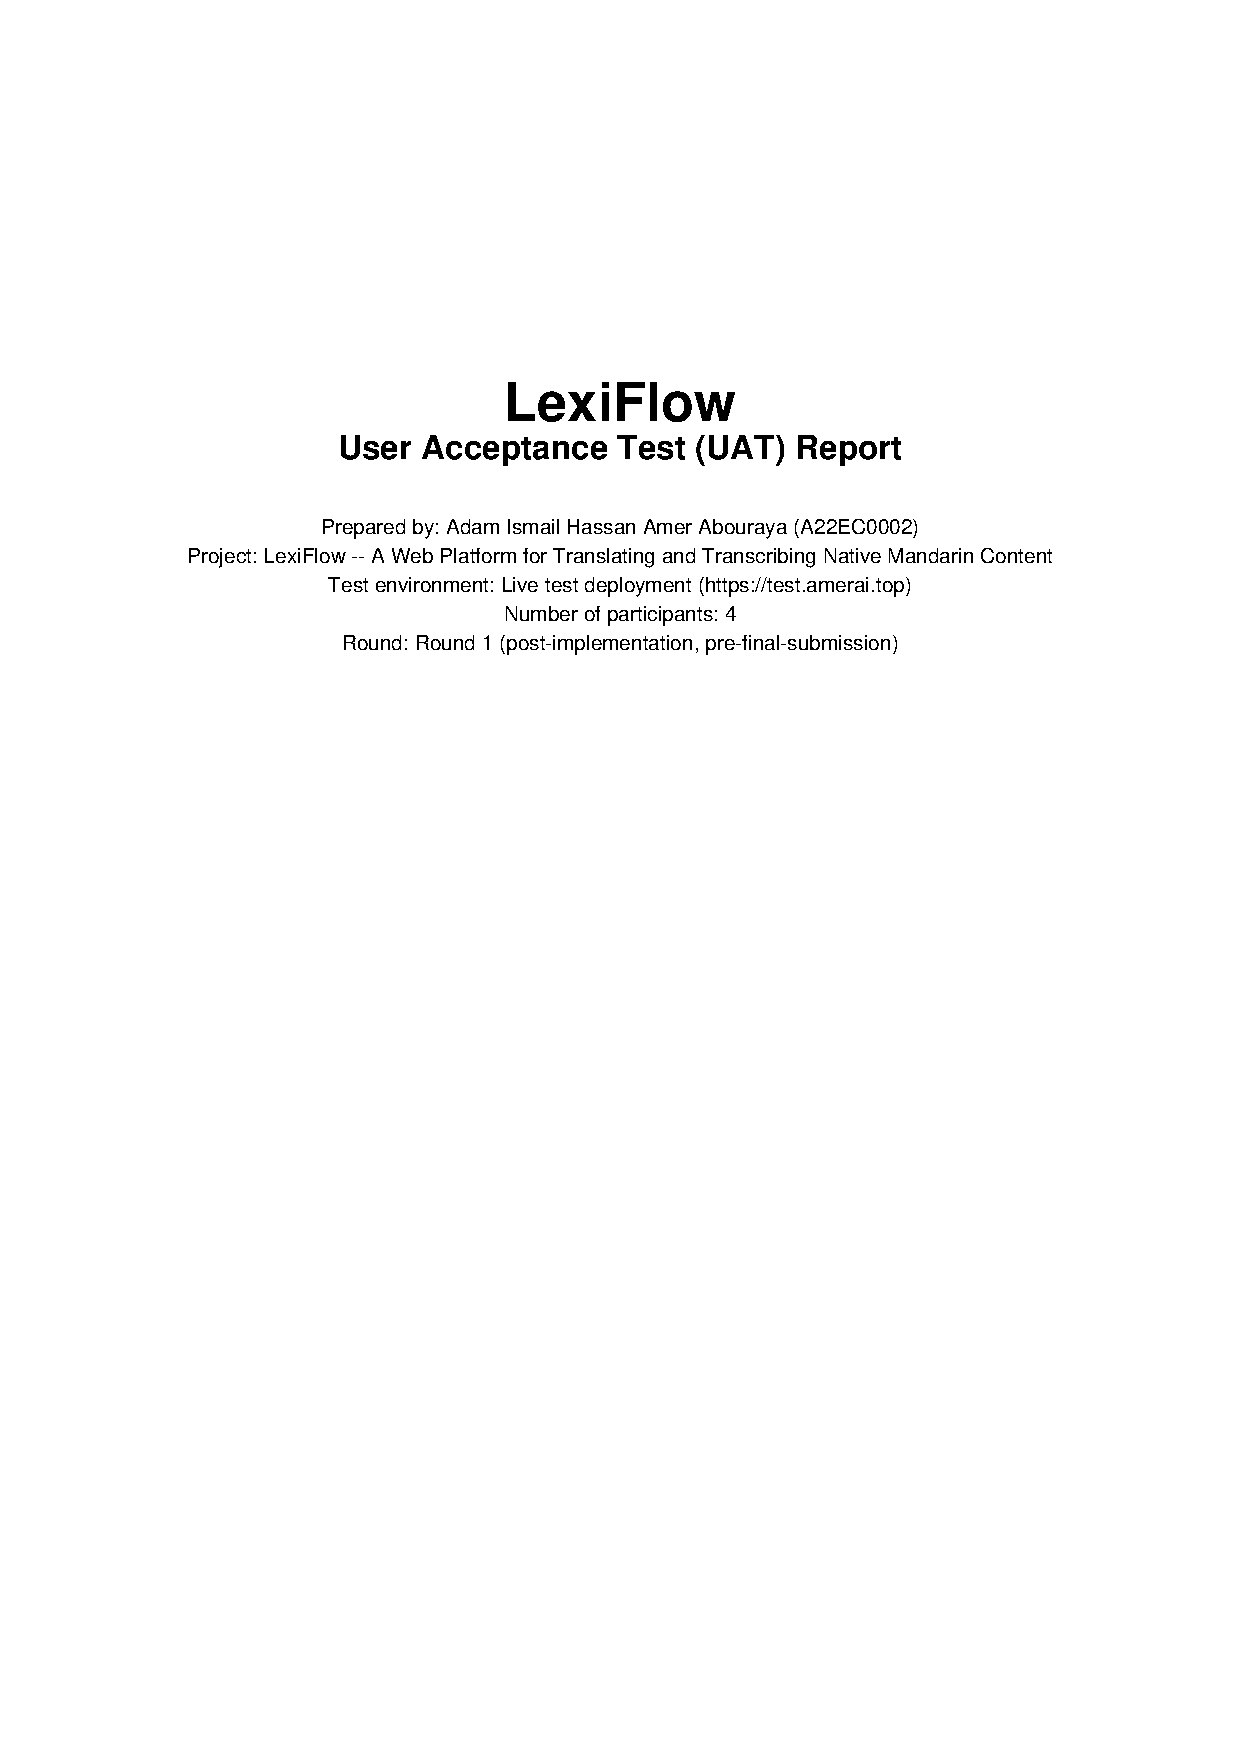
\includepdf[pages=-]{figs/uat_report.pdf}

\chapter{Stakeholder Interview Questions}\label{app:stakeholder-interview-questions}
\pdfbookmark[0]{Stakeholder Interview Questions}{sec:stakeholder-interview-questions}


\section{Teaching Context \& Methods}
\noindent How many students do you typically teach per semester?\\
=\textgreater{} around 180–200 students


\noindent What proficiency levels do you teach (beginner, intermediate, advanced)? What is their HSK level?\\
=\textgreater{} all classes here in UTM language academy teach beginner level Mandarin. The student reaches HSK 1 by the time they finish the subject.

\noindent How do you currently incorporate authentic content into your curriculum? \\
=\textgreater{} as support material. After finishing the lesson slides. The students watch a video or two. The videos are usually kindergarten songs.

\noindent What challenges do you face when preparing authentic content materials?\\
=\textgreater{} the biggest challenge is to find material with the correct level for the students. If it is too difficult or too simple then the students will not learn much.

\section{Content Processing \& Management}
\noindent  How much time do you spend creating subtitles/transcriptions for videos?\\
=\textgreater{} 10–30 mins for simple 3-minute videos

\noindent What types of authentic content work best for different proficiency levels?\\
=\textgreater{} for beginner levels, kindergarten songs are the best choice. However, a lot of students find them childish or boring. Movies are great for more advanced levels. Travel vlogs are also a nice content for beginner/ intermediate levels.

\noindent How do you currently assess student comprehension of authentic materials?\\ =\textgreater{} by using quizzes. Both in class and online quizzes on e-learning. Listening quizzes are the best but mcq is also usable.

\section{Quality \& Accuracy Requirements}
\noindent What level of transcription accuracy is acceptable for educational use?\\
=\textgreater{} above 90\% is acceptable

\noindent What quality control measures should be in place?\\
=\textgreater{} as long as the model or translation service used is backed by good research then this should good enough for such projects

\noindent How important is consistency in pinyin romanization systems?\\
=\textgreater{} it is important but not the most important part of this system. Having correct translation is the most important feature in this system.

\chapter{Feedback on Prototype Meeting with Stakeholder}\label{app:feedback-on-prototype}
\pdfbookmark[0]{Feedback on Prototype Meeting with Stakeholder}{sec:feedback-on-prototype}

Saya telah pun mengadakan pertemuan dengan Adam. Beliau telah membentangkan prototype tersebut.~\href{https://lexiflow.amerai.top}{[Prototype Link]}.

\section{Maklumbalas saya adalah seperti berikut:}

\begin{enumerate}[label=\arabic*.]
    \item Secara keseluruhannya sistem tersebut berfungsi dengan baik.
    \item Hasil transcribing video yang ditunjukkan adalah tepat, melebihi 95\%.
    \item Ketepatan terjemahan juga adalah melebihi 90\%.
    \item Features seperti terjemahan per kosa kata adalah tepat dan membantu.
    \item Setiap kosa kata mempunyai label tahap HSK (Chinese Proficiency Test), ia membantu untuk rujukan pengguna.
    \item Sistem tersebut sangat mudah untuk digunakan.
    \item Prototype ini sesuai untuk digunakan untuk pengajar dan pelajar bagi tujuan pembelajaran bahasa mandarin.
\end{enumerate}

\section{Terdapat 2 masalah utama:}

\subsection{Terjemahan}
\begin{enumerate}[label=\arabic*.]
    \item Ketepatan terjemahan terganggu pada video yang mempunyai kandungan bahasa rojak (Mandarin-English, Mandarin-Malay).
    \item Frasa yang mempunyai maksud tersirat atau bergantung pada konteks budaya sedikit mempengaruhi ketepatan terjemahan.
    \item Kata ulangan (bentuk jamak) sering terlepas untuk ditranskrip secara penuh, namun ia tidak mengganggu terjemahan ayat secara keseluruhannya.
\end{enumerate}

\subsection{Kegagalan Transcribing}
Kami mendapati terdapat video yang tidak berjaya untuk transcribe. Kami menjangkakan terdapat beberapa sebab:
\begin{enumerate}[label=\arabic*.]
    \item Suara talent yang bercakap tidak jelas atau tidak kuat.
    \item Berlaku code-switching (Mandarin-English-Malay) yang terlalu kerap.
    \item Talent bercakap terlalu laju.
\end{enumerate}

\section{Cadangan dan Penambahbaikan:}
\begin{enumerate}[label=\arabic*.]
    \item Perlu uji lebih banyak video yang mempunyai slang atau dialect yang berbeza.
    \item Feature "Recommended Videos" perlu di label mengikut kesesuaian tahap penguasaan bahasa pengguna.
    \item Penambahan features untuk penilaian pengguna, seperti flashcard, quiz dan lain-lain.
    \item Sekiranya tujuan utama sistem ini adalah untuk pembelajaran, tambah features playlists yang bertema bagi memastikan pembelajaran lebih tersusun dan berstruktur.
\end{enumerate}

\begin{flushleft}
    \textbf{MUHAMMAD ZAID BIN MUHAMMAD SHAFIE} \\
    Foreign Language Coordinator \\
    Mandarin Language Instructor \\
    Language Academy \\
    Faculty of Social Sciences and Humanities \\
    UTM, Johor Bahru \\
    Email: m.zaid@utm.my
\end{flushleft}


% \chapter{Project Timeline Management with Jira}\label{app:project-timeline-management-with-jira}
% \pdfbookmark[0]{Project Timeline Management with Jira}{sec:project-timeline-management-with-jira}

\chapter{Software Requirements Specification (SRS)}\label{app:srs}
\pdfbookmark[0]{SRS}{sec:srs}
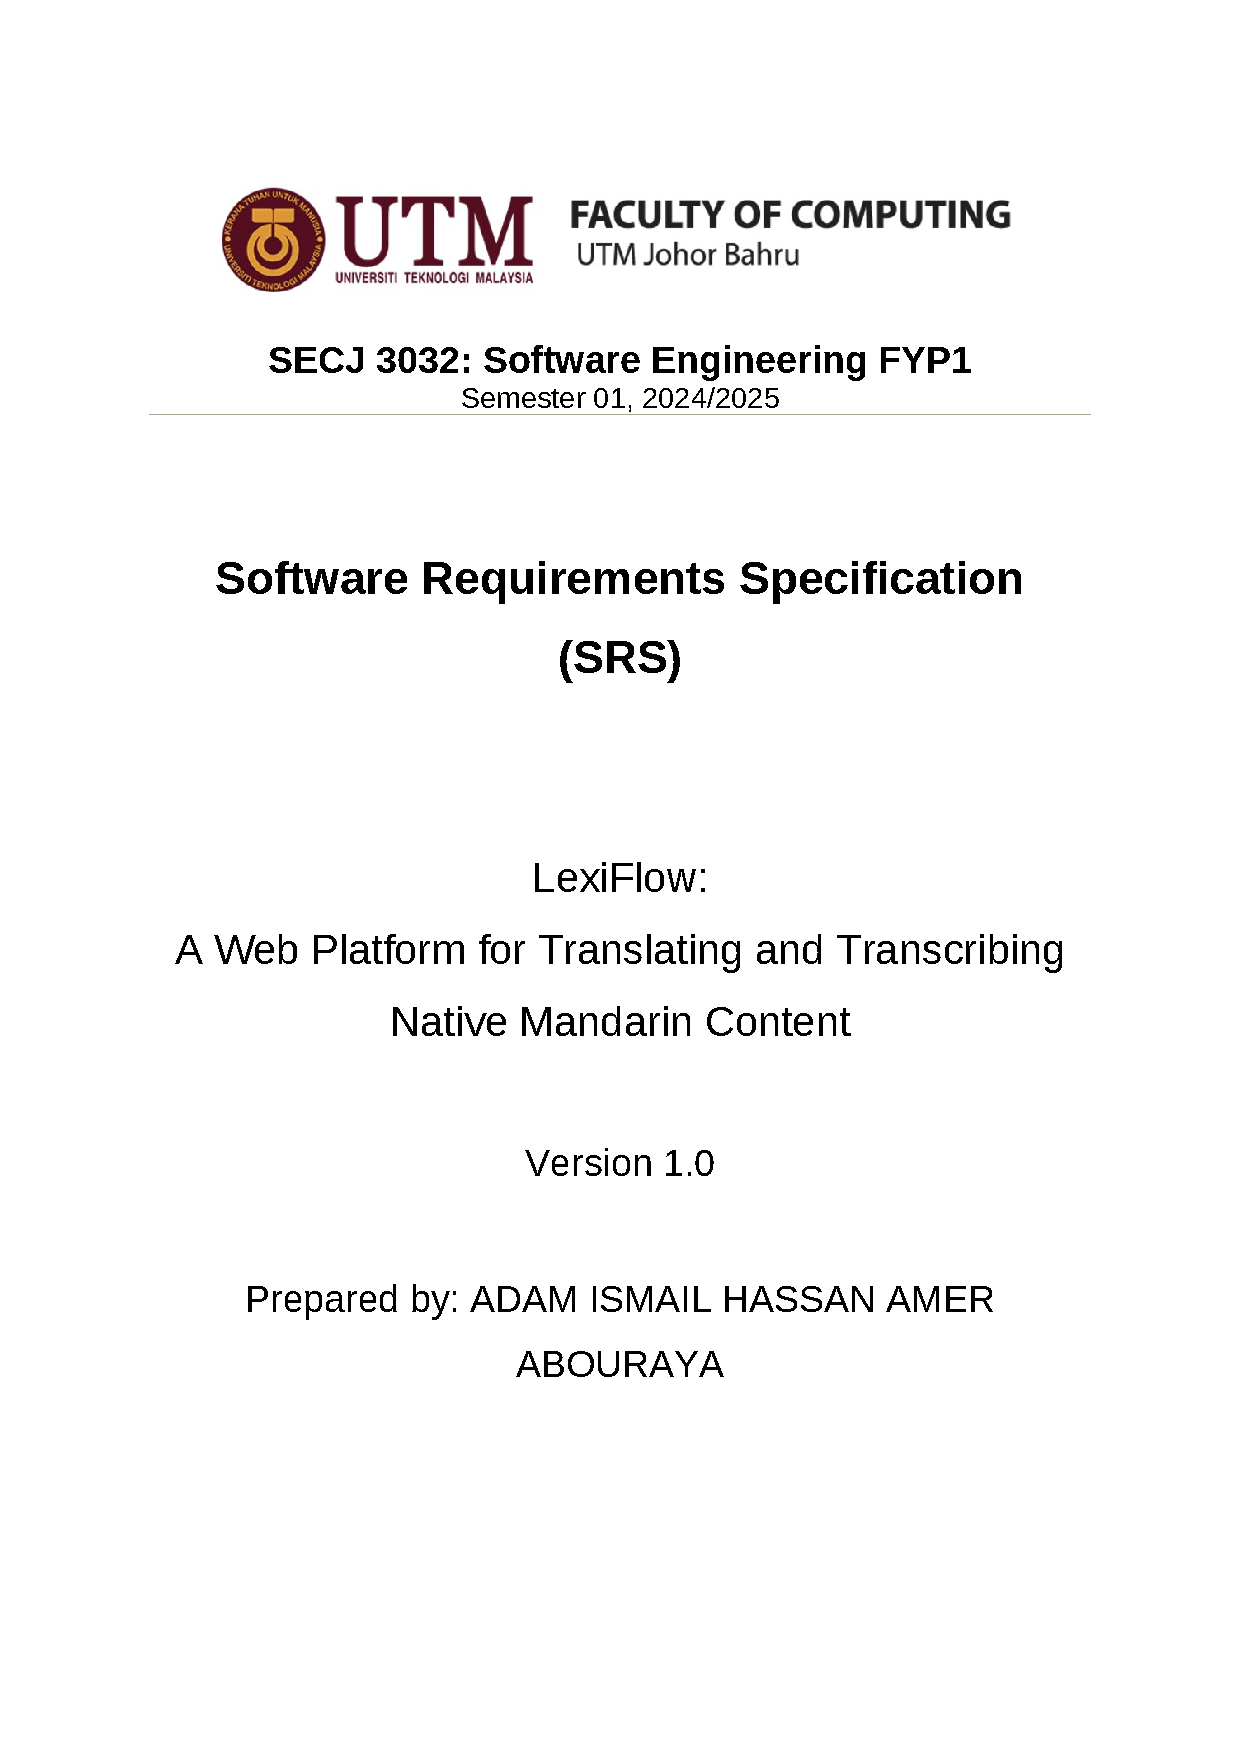
\includepdf[pages=-]{figs/srs.pdf}
\chapter{Software Design Document (SDD)}\label{app:sdd}
\pdfbookmark[0]{SDD}{sec:sdd}
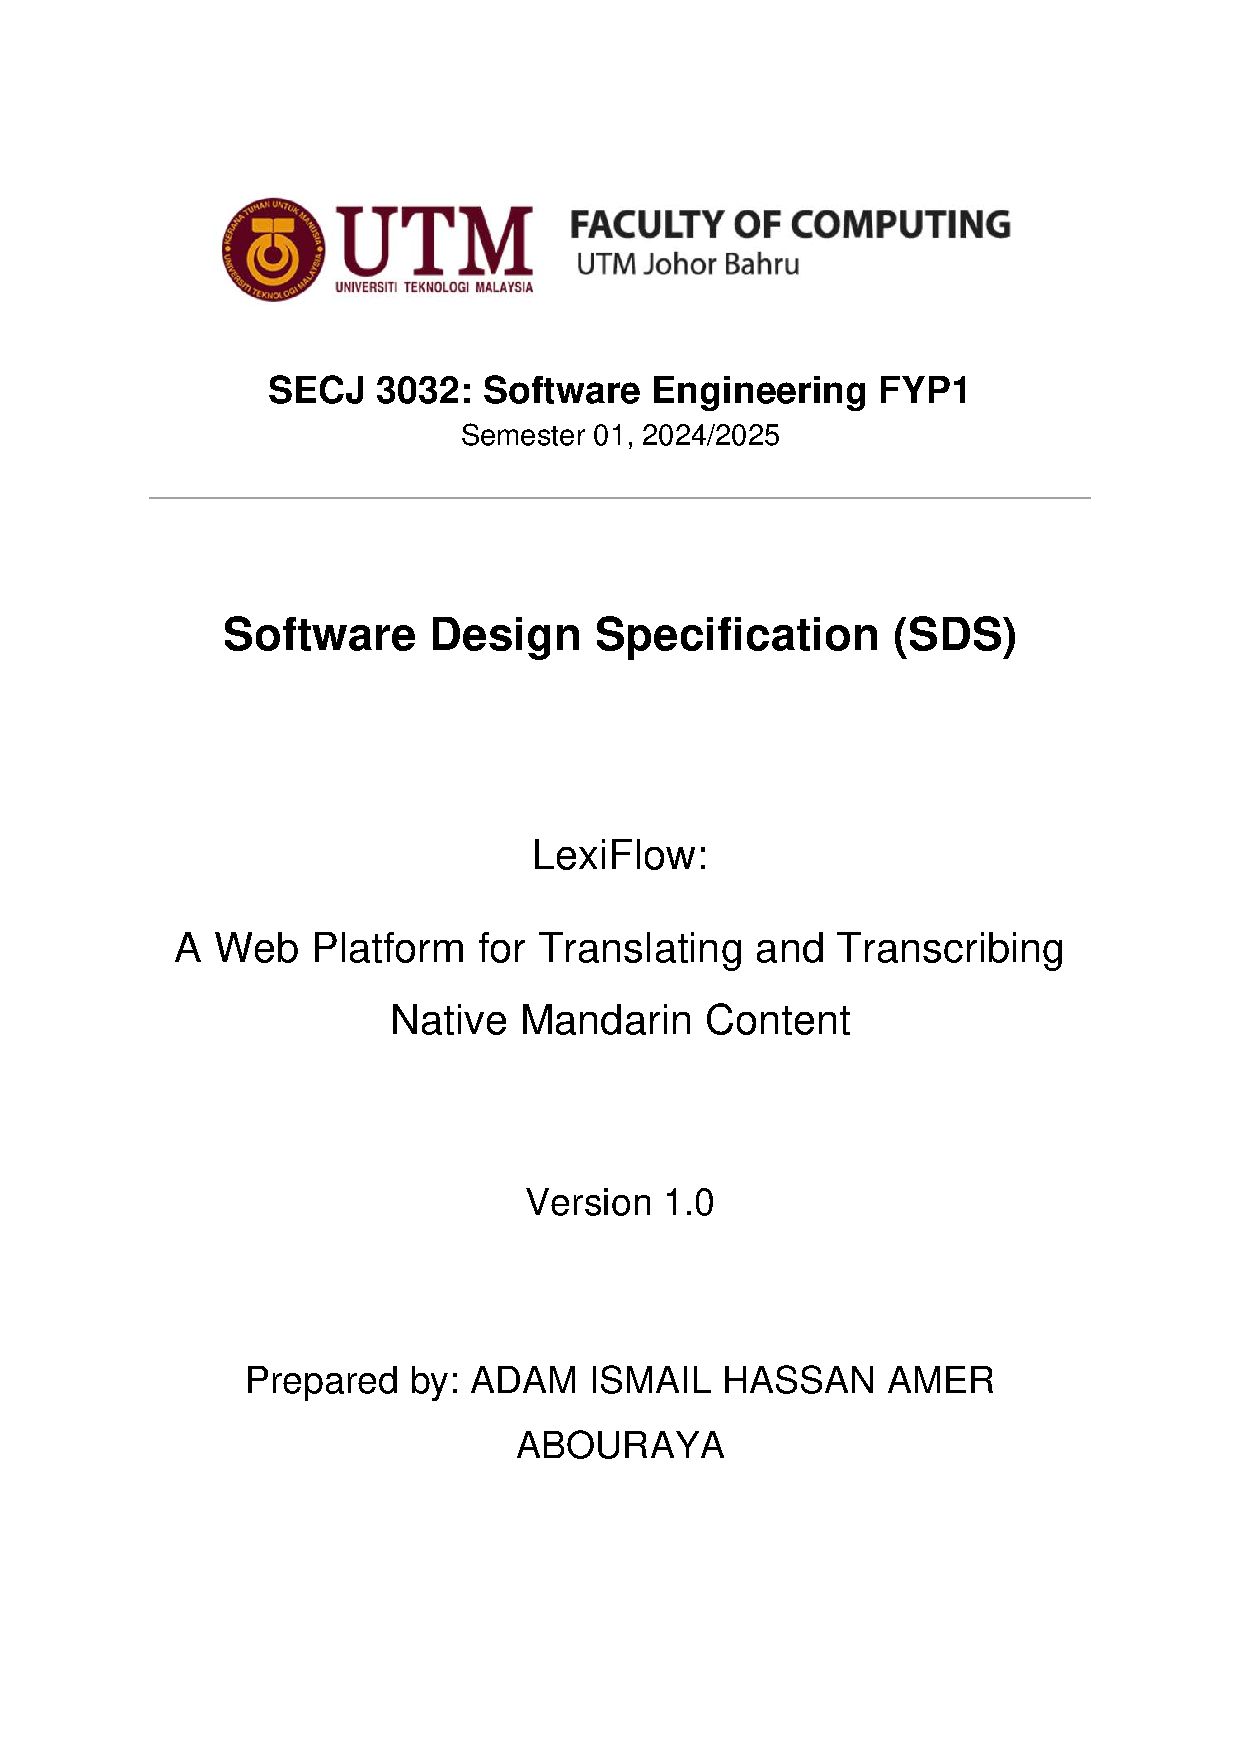
\includepdf[pages=-]{figs/sdd.pdf}
\chapter{Software Testing Document (STD)}\label{app:std}
\pdfbookmark[0]{STD}{sec:std}
% \includepdf[pages=-]{figs/std.pdf}
\hspace{\fill}


%This is required to make List of Appendices possible. Remove when have no appendix.
\endmatter
\end{document}
